\chapter{Producing Elevation Confidence Intervals}\label{chap:elevation_intervals}
In \Cref{chap:epistemic_uncertainty}, we presented a method for computing disparity confidence intervals alongside each predicted disparity $\tilde{d}$. In the photogrammetry pipeline, the predicted disparity is triangulated, filtered (\Cref{sec:triangulation}) and then rasterized (\Cref{sec:rasterization}) to obtain the final \acrshort{dsm}. We will see in this chapter how we can apply those steps to disparity confidence intervals in order to propagate them into elevation confidence intervals, associated with the \acrshort{dsm} values. This chapter takes up work and data published in \cite{malinowski_robust_2024}.

In \Cref{sec:related_work} of \Cref{chap:stereophotogrammetry}, we presented related work where confidence intervals were computed based on a \acrshort{dsm}, mainly in \cite{oksanen_digital_2006,panagiotakis_validation_2018,deschamps-berger_apport_2021}. In those studies, a single global confidence interval associated with a \acrshort{dsm} is computed \textit{a posteriori}, \ie based solely on the \acrshort{dsm} (and reference points), regardless of the method used to obtain it (\ie, photogrammetry, \acrshort{lidar}, \acrshort{radar}). The methodology presented in this chapter estimates the uncertainty independently for each pixel, leading to small confidence intervals in confident areas, and bigger confidence intervals where the algorithms may have performed badly. We differ in this regard to previous work, and it does not seem relevant to compare our intervals to theirs, as their most similar characteristics is their name ``interval'', but neither share the same form (single \vs multiple intervals), nor are based on the same data.

\section{From Disparity Intervals to Elevation Intervals}\label{sec:elevation_intervals}
\subsection{Triangulation of Disparity Intervals}
As indicated by their name, disparity confidence intervals are expressed in pixel of disparities. Disparities are used to determine  pairs of intersecting lines of sight from different sensors, which are then triangulated to obtain a 3D point. With disparity confidence intervals, we now have 3 pairs of line of sight for each pixel instead of just one:
\begin{itemize}
    \item The pair composed using the predicted disparity $\tilde{d}$
    \item The two pairs composed using the upper and lower disparities from $I_\alpha=[\underline{I}_\alpha, ~\overline{I}_\alpha]$.
\end{itemize}
Intersecting each pair of line of sight yields $3$ 3D points, as presented in \Cref{fig:pairs_of_line_of_sight}. We deduce the first point $(x, ~y, ~z)$ from predicted disparity $\tilde{d}$, and the two other points $(\underline{x}, ~\underline{y}, ~\underline{z})$, $(\overline{x}, ~\overline{y}, ~\overline{z})$ are deduced from $\underline{I}_\alpha$ and $\overline{I}_\alpha$ respectively.
\begin{figure}
    \centering
    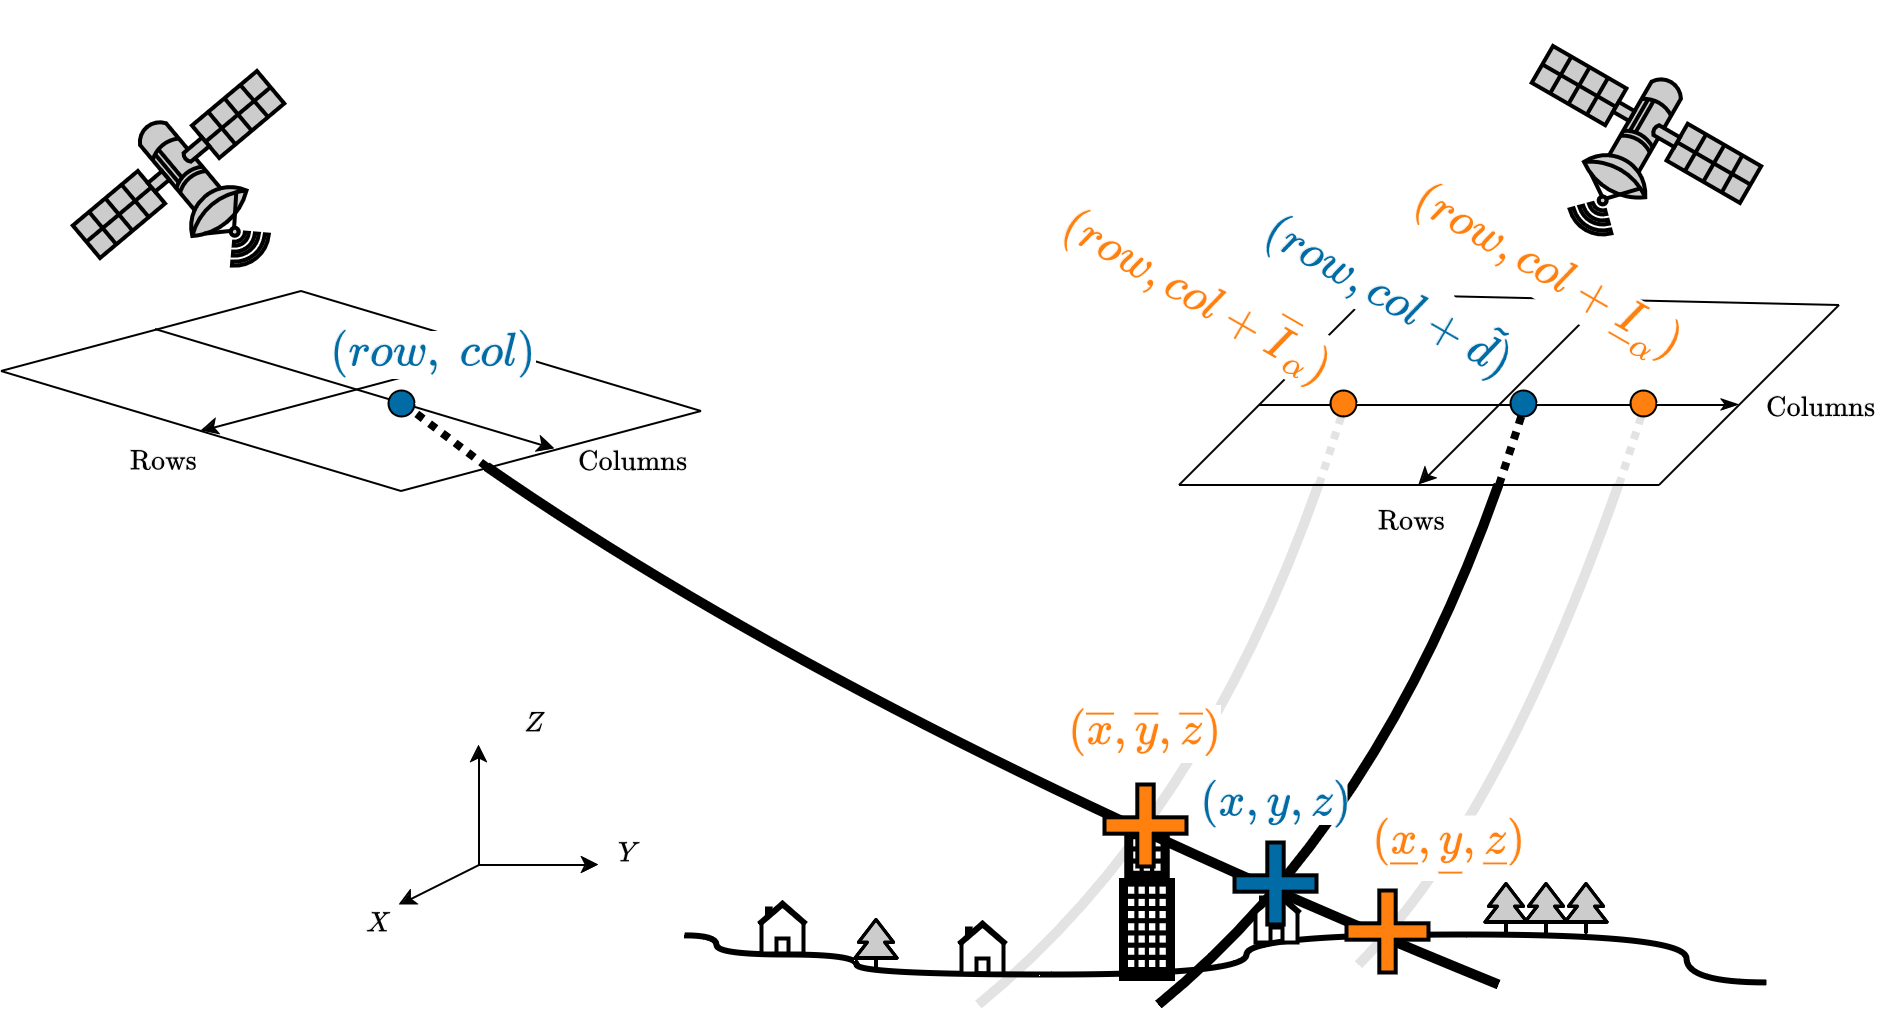
\includegraphics[width=\linewidth]{Images/Chap_6/Pairs_of_line_of_sight.png}
    \caption{Triangulation of the three pairs of lines of sight. The angle between lines of sight is exaggerated for the purpose of this illustration.}
    \label{fig:pairs_of_line_of_sight}
\end{figure}

Depending on the disposition of satellites, as well as which image is selected as the reference image, it is both possible that $\overline{z}\leqslant z \leqslant \underline{z}$ or $\underline{z}\leqslant z \leqslant \overline{z}$. In the following, and for simplicity, we will consider that $\underline{z}\leqslant z \leqslant \overline{z}$. This is not constraining, as we can just change the notations to unsure this inequality holds. We therefore have a 3D confidence ``interval'', defined as every point from the reference line of sight between $(\underline{x}, ~\underline{y}, ~\underline{z})$ and $(\overline{x}, ~\overline{y}, ~\overline{z})$. For instance in \Cref{fig:pairs_of_line_of_sight}, the reference line of sight is the one originating from the left satellite, and the confidence ``interval'' is the portion of this line of sight between the two orange crosses. It is not an interval \textit{per se}, as \acrshort{rpc} are polynomials and not straight lines, but they are approximated by straight lines in the computations, so the distinction is superfluous. 

The point cloud obtained from the triangulation of the disparity map is then filtered, as detailed in \Cref{sec:triangulation}. If a 3D point is filtered, then we naturally also filter its corresponding interval with it. 

\subsection{Rasterization of 3D ``Intervals''}
The final step of the pipeline is the rasterization, as our objective is to produce elevation confidence intervals associated with every value contained in the \acrshort{dsm}. However, rasterizing intervals along lines of sight as it stands raises an issue: we are not guaranteed that the rasterized intervals will remain coherent with the final \acrshort{dsm} when projected on the regular grid. A solution to circumvent this issue is to consider that the planimetric shift $\Delta XY=\sqrt{(x-\underline{x})^2+(y-\underline{y})^2}$ is small in comparison to the altimetric shift $\Delta Z=\sqrt{(z-\underline{z})^2}$ and that we can therefore neglect it. This hypothesis depends only on the incidence angle $\beta$ of the reference image. Indeed, it holds that $\dfrac{\Delta Z}{\Delta XY}=\dfrac{1}{\tan(\beta)}$, where $\beta$ is the incidence angle as depicted in \Cref{fig:incidence_angle}. Ideally, if the reference image has no incidence angle, then the $\Delta XY$ shift is null. \Cref{tab:angle_coupling_pleiades} details the different incidence angles encountered in our experiments. The incidence angles are typically around $10\degree$, \ie $\Delta Z$ is around $5.6$ times bigger than $\Delta XY$. For the scene in Paris where the incidence reaches $6.1\degree$, the ratio is around $10$, while the only scene with $21.3\degree$, near Peyto Lake, Canada, has a ratio around $2.6$. For this last acquisition, the hypothesis that $\Delta XY$ is small compared to $\Delta Z$ is debatable, but we will still neglect $\Delta XY$ in the rasterization in order to stay consistent across our experiments. This will also allow verifying if this hypothesis can impact the performance of our method.

The lower and upper bounds can thus be aligned directly above and below the predicted 3D point $(x, ~y, ~z)$, and they thus become:
\begin{align}
    (\overline{x}, ~\overline{y}, ~\overline{z}) ~\rightarrow~ (x, ~y, ~\overline{z})\\
    (\underline{x}, ~\underline{y}, ~\underline{z}) ~\rightarrow~ (x, ~y, ~\underline{z})
\end{align}
\Cref{fig:planimetric_shift} illustrates this modification, where the orange points along the line of sight are shifted in the $(X,~Y)$ plane to be vertically aligned with $(x, ~y, ~z)$. 

\begin{figure}
    \centering
    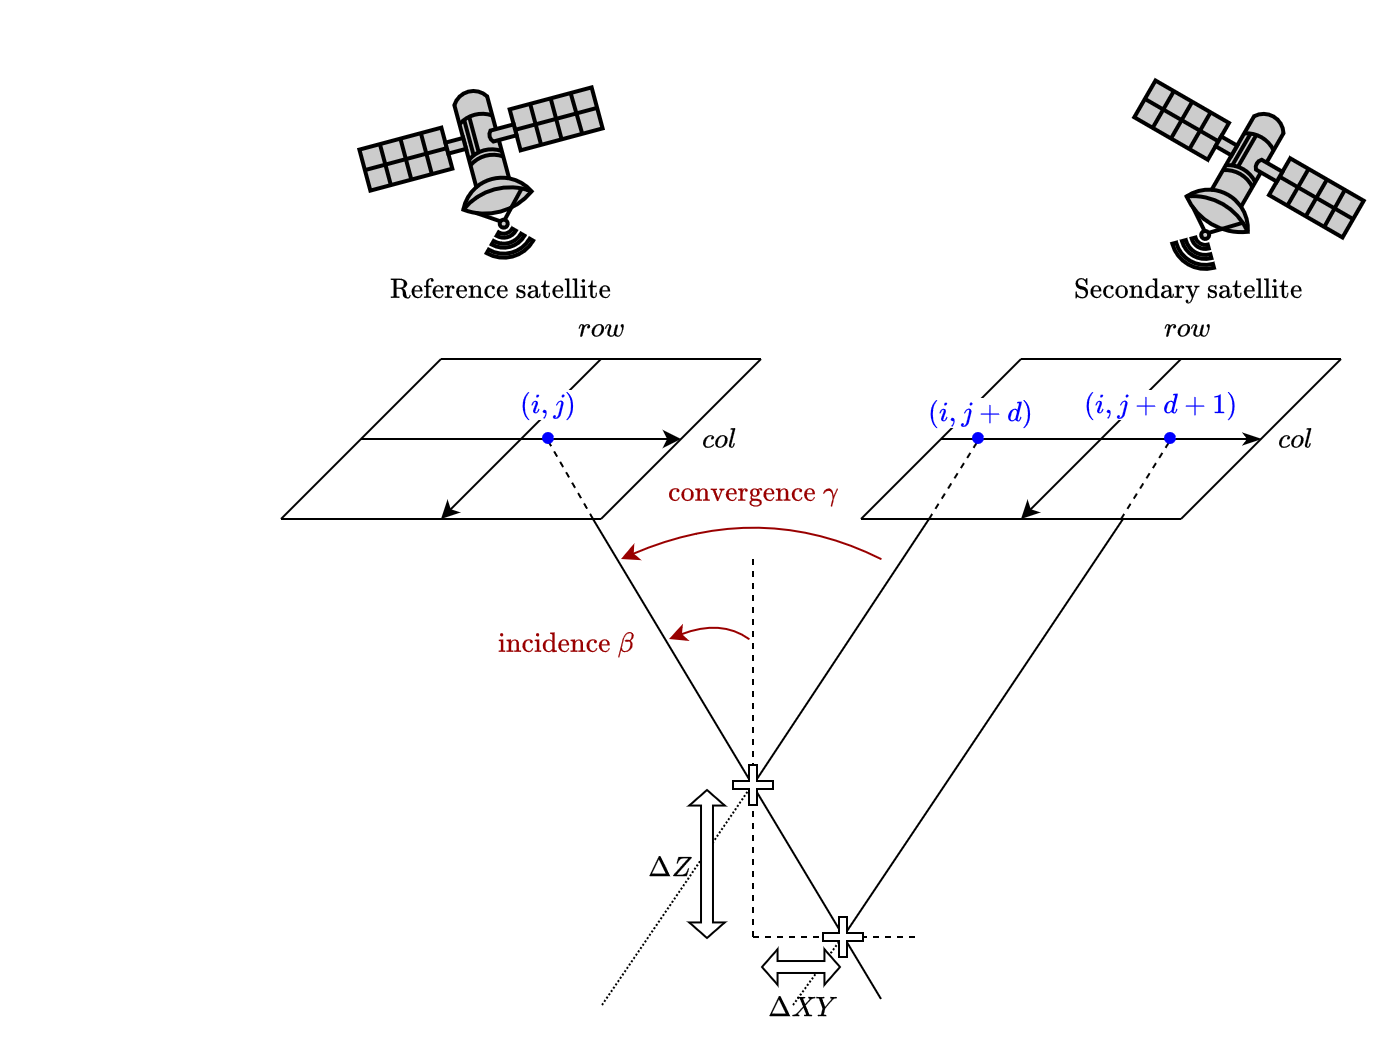
\includegraphics[width=0.8\linewidth]{Images/Chap_6/Incidence_angle.png}
    \caption{Acquisition angles of satellites}
    \label{fig:incidence_angle}
\end{figure}

\begin{figure}
    \centering
    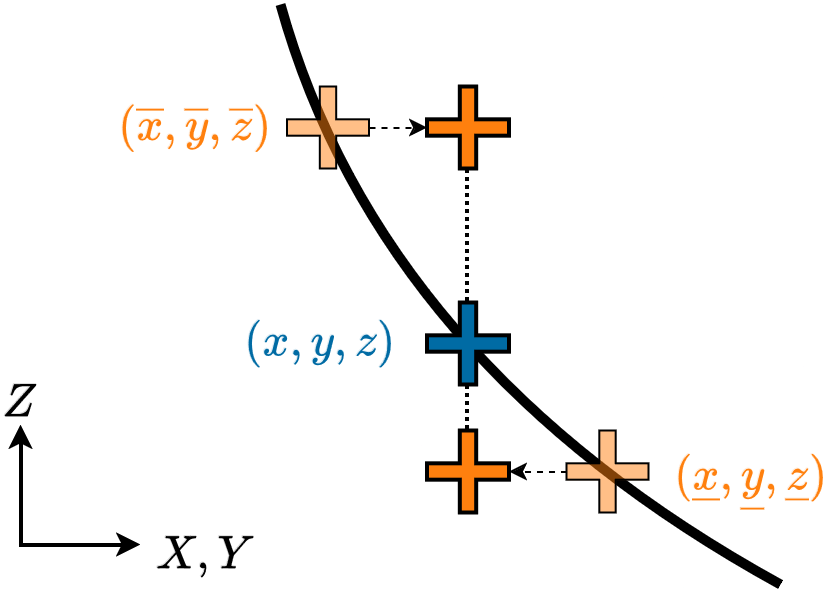
\includegraphics[width=0.6\linewidth]{Images/Chap_6/Planimetric_shift.png}
    \caption{Aligning the confidence interval bounds along a line of sight}
    \label{fig:planimetric_shift}
\end{figure}

We remind here the general formulation of the rasterization step. Let $(x,~y)$ be a cell of the \acrshort{dsm}, and $PC$ be the point cloud considered in the rasterization. The value of the \acrshort{dsm} is computed using a weighted mean of $PC$:
\begin{align}
    \DSM(x,y) &= \dfrac{\sum\limits_{(x_i, y_i, z_i)\in PC}z_i\cdot w(x_i, y_i)}{\sum\limits_{(x_i,y_i,z_i)\in PC} w(x_i, y_i)}
\end{align}
where weights $w(x_i,y_i)$ are positive scalars. In CARS, the weights are computed using a Gaussian distribution, but other pipelines also use Inverse Distance Weightings which works similarly. In practice, only the points within a given distance of the center $(x,y)$ of the cell are considered in the mean. 

Because it holds that for any point: $\underline{z}\leqslant z\leqslant\overline{z}$, then computing the \acrshort{dsm}s independently using $(x, ~y, ~z)$, $(x, ~y, ~\overline{z})$ and $(x, ~y, ~\underline{z})$ will ensure the consistency of the resulting \acrshort{dsm}s:
\begin{eqnarray}
    \dfrac{\sum\limits_{(x_i, y_i, \underline{z}_i)\in PC}\underline{z}_i\cdot w(x_i, y_i)}{\sum\limits_{(x_i,y_i, \underline{z}_i)\in PC} w(x_i, y_i)}
    \leqslant&
    \dfrac{\sum\limits_{(x_i, y_i, z_i)\in PC}z_i\cdot w(x_i, y_i)}{\sum\limits_{(x_i,y_i,z_i)\in PC} w(x_i, y_i)}
    &\leqslant
    \dfrac{\sum\limits_{(x_i, y_i, \overline{z}_i)\in PC}\overline{z}_i\cdot w(x_i, y_i)}{\sum\limits_{(x_i,y_i,\overline{z}_i)\in PC} w(x_i, y_i)}\nonumber\\
    &&\nonumber\\
    \underline{\DSM}(x,y) \leqslant& \DSM(x,y) &\leqslant\overline{\DSM}(x,y)
\end{eqnarray}
where $\underline{\DSM}(x,y)$ is the \acrshort{dsm} computed using points $(x, ~y, ~\underline{z})$, and $\overline{\DSM}(x,y)$ is the \acrshort{dsm} computed using points $(x, ~y, ~\overline{z})$. For each cell $\DSM(x,y)$ we have now computed an elevation interval $[\underline{\DSM}(x,y),~\overline{\DSM}(x,y)]$.

As rasterization is the final step of the stereo pipeline, we now have propagated the confidence intervals all the way to the end of the pipeline while ensuring their coherency with the predicted \acrshort{dsm}. Additionally, The production of elevation confidence intervals did not influence the values of the final \acrshort{dsm}. We now need to evaluate the elevation confidence intervals on real data to verify if the potential errors occurring during the transformation of disparity intervals into elevation intervals do not question their accuracy.

\section{Acquiring and Processing Data for Evaluation}
\subsection{Satellite and DSM datasets}
This section will present the different images and ground truth \acrshort{dsm}s used to evaluate elevation intervals. We will use ground truth \acrshort{dsm}s that can be categorized into two categories.

The first category is composed of \acrshort{dsm}s acquired over mountainous regions containing glaciers. They have been kindly provided by Etienne Berthier from LEGOS, Liss Marie Andreassen from the Norwegian Water Resources and Energy Directorate (NVE) and Brian Menounos from the Natural Sciences and Engineering Research Council of Canada and the Tula Foundation (Hakai Institute). The data were acquired in the following regions:
\begin{itemize}
    \item Two different \acrshort{dsm}s in the mountainous region of Jotunheinem, Norway. We will refer to the two \acrshort{dsm}s as Hellmem (\Cref{fig:miniature_Hellmem}) and Graasubreen (\Cref{fig:miniature_Graasubreen}).
    \item Langfjordjøkelen glacier, Norway (\Cref{fig:miniature_Langfjordjokelen}).
    \item Mountains near Peyto lake, in the Alberta province of Canada. (\Cref{fig:miniature_Peyto})
\end{itemize}
The ground truth were acquired using a \acrshort{lidar} sensor, rasterized at 50 cm resolution. We did not apply the rasterization ourselves and only had access to the rasterized \acrshort{dsm}s.

The second category of ground truth data comes from the \acrshort{lidar} HD program (\cite{monnet_lidarhd_2023}, \url{https://geoservices.ign.fr/lidarhd}) which intends to cover the entirety of the French territory (except for French Guiana) by the end of 2026. It is a very important source of information, with around $10$ measured points per m$^2$ and a relative planimetric accuracy of 50 cm. As of the time we write this thesis, data over the French territory are not fully (publicly) available. From the data available at the time of this work, we selected different regions of interest in order to have a variety of landscapes (rural, urban, seaside \etc). Those landscapes all presented strong elevation variations in order to present a challenge for the stereo pipeline. We also want to determine if our method behaves differently depending on the nature of the scene. Here is the list of the considered regions:
\begin{itemize}
    \item The city of Bordeaux (\Cref{fig:miniature_Bordeaux})
    \item The city of Montpellier (\Cref{fig:miniature_Montpellier})
    \item The city of Paris (\Cref{fig:miniature_Paris})
    \item The city of Toulouse (\Cref{fig:miniature_Toulouse})
    \item Valleys and mountains near Grenoble, in the French Alps (\Cref{fig:miniature_Grenoble})
    \item Mediterranean coastline with the city of Monaco (\Cref{fig:miniature_Monaco})
    \item Valleys and mountains at Pic du Midi, french Pyrenees (\Cref{fig:miniature_pic_du_midi})
\end{itemize}
\acrshort{lidar} point clouds were then rasterized at 50 cm resolution with the same Gaussian rasterization method as in the stereo pipeline. \Cref{tab:dates_pleiades_lidar_hd} presents the different acquisition dates and shape of the ground truth \acrshort{dsm}s.

We used Pléiades images for producing both \acrshort{dsm}s and intervals that will be compared to the ground truth. We did not directly order the Pléiades acquisitions, as it is costly and hard to synchronize with the acquisition date of the ground truth. From our available catalog, we selected stereo pairs that were acquired as close as possible from the acquisition date of the ground truth, or if multiple months separated the two acquisitions, we rather selected a similar period of the previous/next year to minimize seasonal changes. \Cref{tab:dates_pleiades_lidar_hd} allows comparing dates of acquisition of the \acrshort{lidar} and Pléiades images.

We saw in \Cref{sec:elevation_intervals} that the planimetric and altimetric accuracy depend on the incidence and convergence angles of the lines of sights of the satellites. \Cref{tab:angle_coupling_pleiades} presents those angles for the different Pléiades images.

\begin{table}[ht]
    \centering
    \begin{tabular}{|c||c|c|c|}
    \hline
        Area & Date for LiDAR & Date of Pléiades &  GT Size (0.5m)\\
        \hline\hline
        Bordeaux & 2023-09-15 & 2022-08-04 & $6001\times 6001$\\\hline
        Grenoble & 2021-09-05 & 2020-09-17 & $10 001\times 10 001$ \\\hline
        Hellmem 1 & 2019-08-27 & 2019-08-27 & $7127\times 7298$ \\\hline
        Graasubreen 2 & 2019-08-27 & 2019-08-27 & $3912\times2880$ \\\hline
        Langfjordjøkelen & 2018-09-01 & 2018-09-01 & $5841\times 3689$\\\hline
        Monaco & 2021-05-13 & 2020-08-30 & $10 001\times 10 001$\\\hline
        Montpellier & 2021-05-28 & 2021-10-17 & $8001\times 8001$\\\hline
        Paris & 2023-03-03 & 2023-05-31 & $10 001\times 10 001$\\\hline
        Peyto & 2016-09-13 & 2016-09-13 & $13240\times 17874$\\\hline
        Pic du Midi & 2021-10-02 & 2021-10-16 & $10001 \times 12001$ \\\hline
        Toulouse & 2022-05-29 & 2022-06-28 & $12001\times 8001$\\\hline
    \end{tabular}
    \caption{Acquisition date of Pléiades stereo or tri-stereo images, and the \acrshort{lidar} ground truth}
    \label{tab:dates_pleiades_lidar_hd}
\end{table}

\begin{table}[ht]
    \centering
    \begin{tabular}{|c||c|c|c|c|}
        \hline
        Area & Convergence angle & Left incidence angle & Right incidence angle \\
        \hline\hline
        Bordeaux & 23.1\degree & 9.7\degree & 14.2\degree \\\hline
        Grenoble & 28.3\degree & 12.4\degree & 16.1\degree \\\hline
        Jotunheinem & 22.5\degree & 10.6\degree & 14.5\degree \\\hline
        Langfjordjøkelen & 21.4\degree & 10.2\degree & 13.8\degree \\\hline
        Monaco & 29.2\degree & 12.8\degree & 18.1\degree \\\hline
        Montpellier & 7.7\degree & 11.5\degree & 15\degree\\\hline
        Paris & 4.9\degree& 6.1\degree & 7.9\degree\\\hline
        Peyto & 17.2\degree & 21.3\degree & 21.6\degree \\\hline
        Pic du Midi & 29.0\degree & 13.7\degree & 15.3\degree \\\hline
        Toulouse & 11.4\degree & 12.5\degree & 18.7\degree\\\hline
    \end{tabular}
    \caption{Relevant angles of stereo pairs of Pléiades images. See \Cref{fig:incidence_angle} for a schematic representation of those angles.}
    \label{tab:angle_coupling_pleiades}
\end{table}

\begin{figure}
    \centering
    \begin{subfigure}[t]{0.48\linewidth}
        \flushleft
        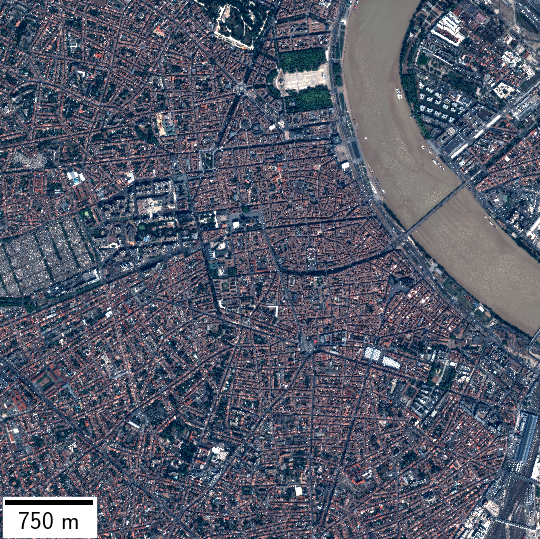
\includegraphics[width=\linewidth]{Images/Chap_6/miniature_Bordeaux.png}
        \caption{\acrshort{rgb} image of Bordeaux (Pléiades © \acrshort{cnes} 2022, Distribution AIRBUS DS)}
        \label{fig:miniature_Bordeaux_rgb}
    \end{subfigure}\hfill
    \begin{subfigure}[t]{0.48\linewidth}
        \flushright
        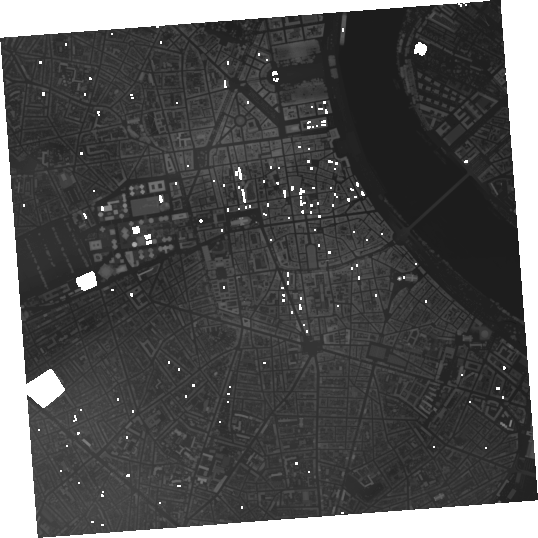
\includegraphics[width=\linewidth]{Images/Chap_6/miniature_Bordeaux_gt.png}
        \caption{\acrshort{lidar} HD \acrshort{dsm}}
        \label{fig:miniature_Bordeaux_gt}
    \end{subfigure}
    \caption{\acrshort{rgb} image of Bordeaux and its associated ground truth \acrshort{dsm}.}
    \label{fig:miniature_Bordeaux}
\end{figure}

\begin{figure}
    \centering
    \begin{subfigure}[t]{0.48\linewidth}
        \flushleft
        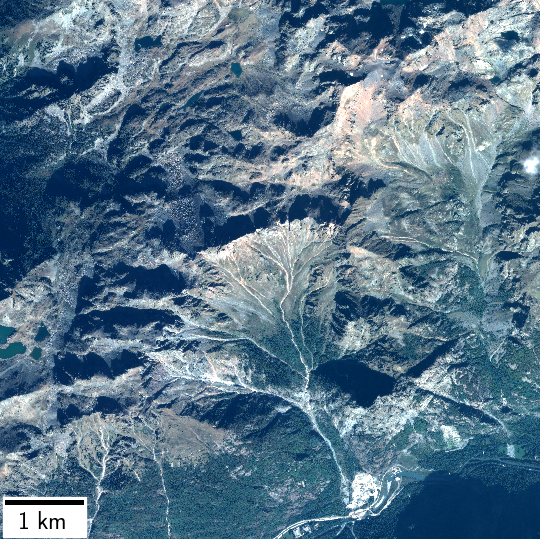
\includegraphics[width=\linewidth]{Images/Chap_6/miniature_Grenoble.png}
        \caption{\acrshort{rgb} image of a region near Grenoble (Pléiades © \acrshort{cnes} 2020, Distribution AIRBUS DS)}
        \label{fig:miniature_Grenoble_rgb}
    \end{subfigure}\hfill
    \begin{subfigure}[t]{0.48\linewidth}
        \flushright
        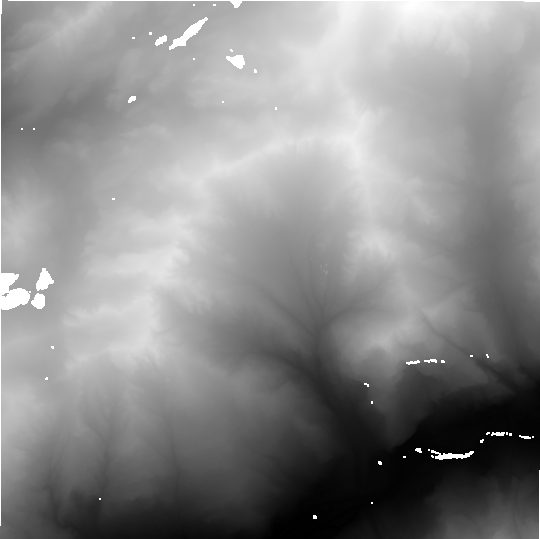
\includegraphics[width=\linewidth]{Images/Chap_6/miniature_Grenoble_gt.png}
        \caption{\acrshort{lidar} HD \acrshort{dsm}}
        \label{fig:miniature_Grenoble_gt}
    \end{subfigure}
    \caption{\acrshort{rgb} image of Grenoble and its associated ground truth \acrshort{dsm}.}
    \label{fig:miniature_Grenoble}
\end{figure}

\begin{figure}
    \centering
    \begin{subfigure}[t]{0.48\linewidth}
        \flushleft
        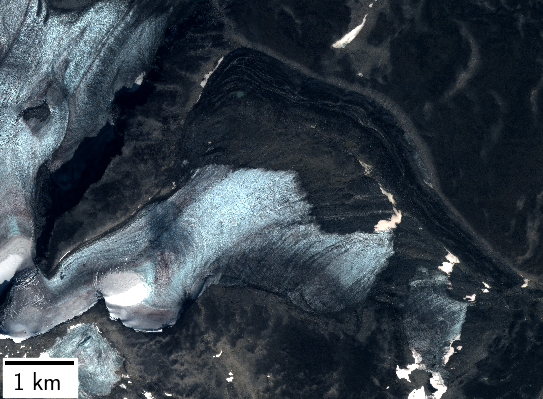
\includegraphics[width=\linewidth]{Images/Chap_6/miniature_Graasubreen.png}
        \caption{\acrshort{rgb} image of Graasubreen (Pléiades © \acrshort{cnes} 2019, Distribution AIRBUS DS)}
        \label{fig:miniature_Graasubreen_rgb}
    \end{subfigure}\hfill
    \begin{subfigure}[t]{0.48\linewidth}
        \flushright
        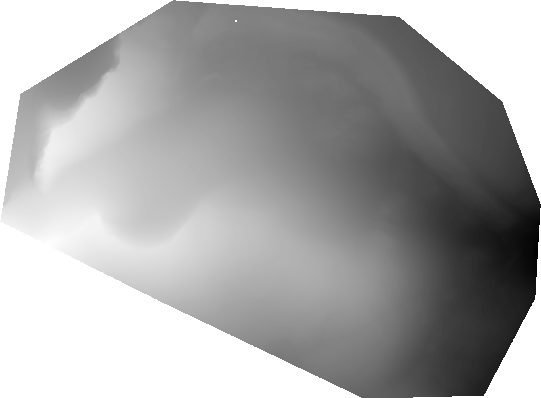
\includegraphics[width=\linewidth]{Images/Chap_6/miniature_Graasubreen_gt.png}
        \caption{\acrshort{lidar} \acrshort{dsm}}
        \label{fig:miniature_Graasubreen_gt}
    \end{subfigure}
    \caption{\acrshort{rgb} image of Graasubreen and its associated ground truth \acrshort{dsm}.}
    \label{fig:miniature_Graasubreen}
\end{figure}

\begin{figure}
    \centering
    \begin{subfigure}[t]{0.48\linewidth}
        \flushleft
        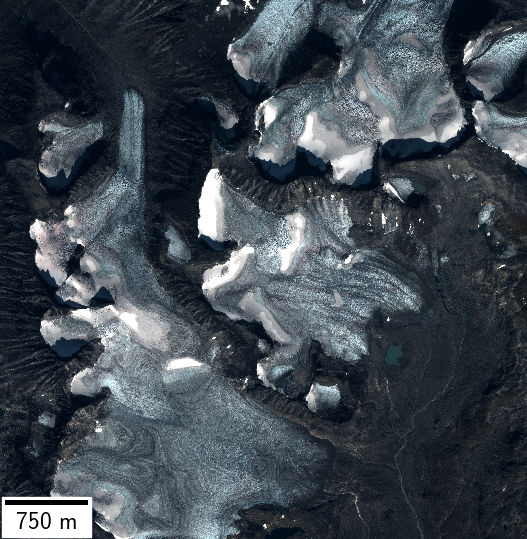
\includegraphics[width=\linewidth]{Images/Chap_6/miniature_Hellmem.png}
        \caption{\acrshort{rgb} image of Hellmem (Pléiades © \acrshort{cnes} 2019, Distribution AIRBUS DS)}
        \label{fig:miniature_Hellmem_rgb}
    \end{subfigure}\hfill
    \begin{subfigure}[t]{0.48\linewidth}
        \flushright
        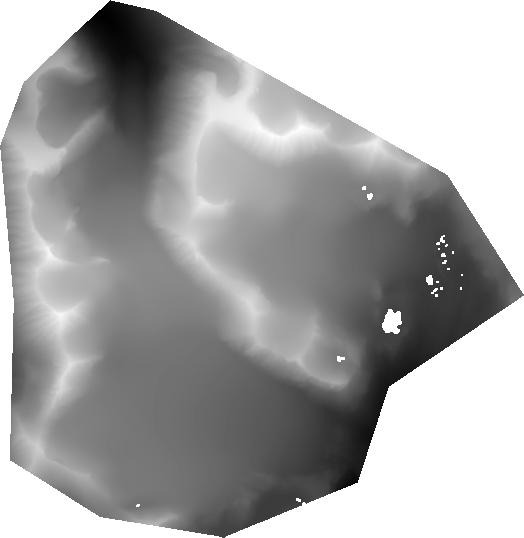
\includegraphics[width=\linewidth]{Images/Chap_6/miniature_Hellmem_gt.png}
        \caption{\acrshort{lidar} \acrshort{dsm}}
        \label{fig:miniature_Hellmem_gt}
    \end{subfigure}
    \caption{\acrshort{rgb} image of Hellmem and its associated ground truth \acrshort{dsm}.}
    \label{fig:miniature_Hellmem}
\end{figure}

\begin{figure}
    \centering
    \begin{subfigure}[t]{0.48\linewidth}
        \flushleft
        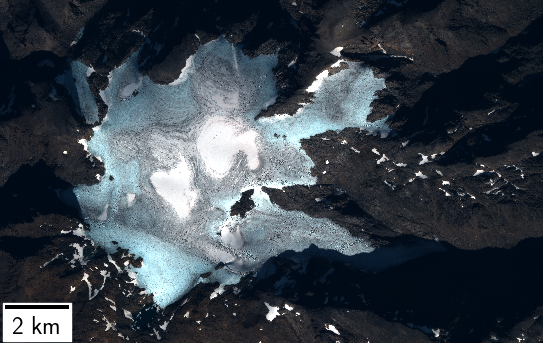
\includegraphics[width=\linewidth]{Images/Chap_6/miniature_Langfjordjokelen.png}
        \caption{\acrshort{rgb} image of Langfjordjøkelen (Pléiades © \acrshort{cnes} 2018, Distribution AIRBUS DS)}
        \label{fig:miniature_Langfjordjokelen_rgb}
    \end{subfigure}\hfill
    \begin{subfigure}[t]{0.48\linewidth}
        \flushright
        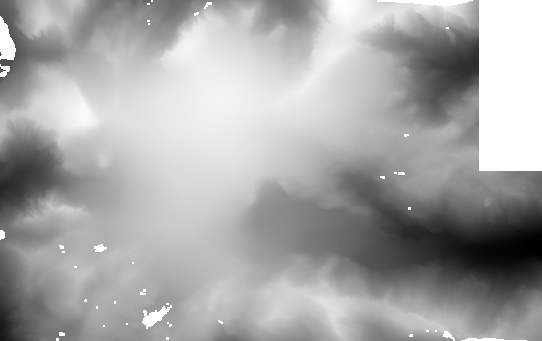
\includegraphics[width=\linewidth]{Images/Chap_6/miniature_Langfjordjokelen_gt.png}
        \caption{\acrshort{lidar} \acrshort{dsm}}
        \label{fig:miniature_Langfjordjokelen_gt}
    \end{subfigure}
    \caption{\acrshort{rgb} image of Langfjordjøkelen and its associated ground truth \acrshort{dsm}.}
    \label{fig:miniature_Langfjordjokelen}
\end{figure}

\begin{figure}
    \centering
    \begin{subfigure}[t]{0.48\linewidth}
        \flushleft
        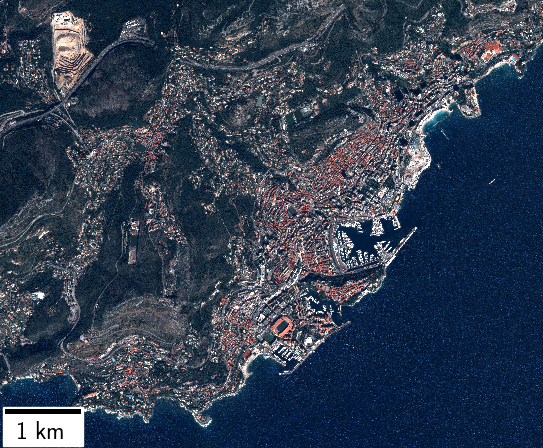
\includegraphics[width=\linewidth]{Images/Chap_6/miniature_Monaco.png}
        \caption{\acrshort{rgb} image of Monaco (Pléiades © \acrshort{cnes} 2020, Distribution AIRBUS DS)}
        \label{fig:miniature_Monaco_rgb}
    \end{subfigure}\hfill
    \begin{subfigure}[t]{0.48\linewidth}
        \flushright
        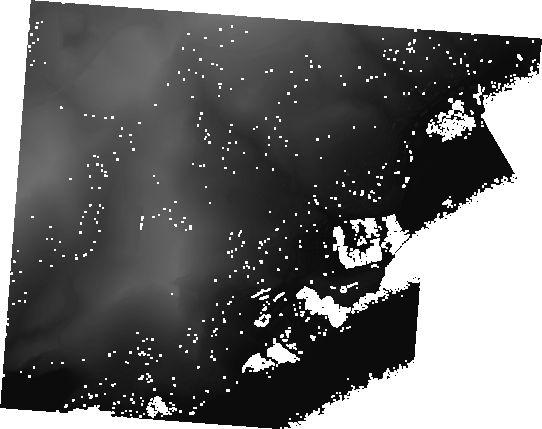
\includegraphics[width=\linewidth]{Images/Chap_6/miniature_Monaco_gt.png}
        \caption{\acrshort{lidar} HD \acrshort{dsm}}
        \label{fig:miniature_Monaco_gt}
    \end{subfigure}
    \caption{\acrshort{rgb} image of Monaco and its associated ground truth \acrshort{dsm}.}
    \label{fig:miniature_Monaco}
\end{figure}

\begin{figure}
    \centering
    \begin{subfigure}[t]{0.48\linewidth}
        \flushleft
        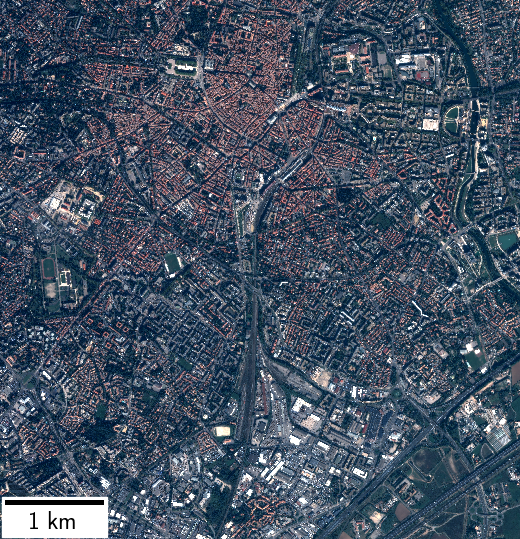
\includegraphics[width=\linewidth]{Images/Chap_6/miniature_Montpellier.png}
        \caption{\acrshort{rgb} image of Montpellier (Pléiades © \acrshort{cnes} 2020, Distribution AIRBUS DS)}
        \label{fig:miniature_Montpellier_rgb}
    \end{subfigure}\hfill
    \begin{subfigure}[t]{0.48\linewidth}
        \flushright
        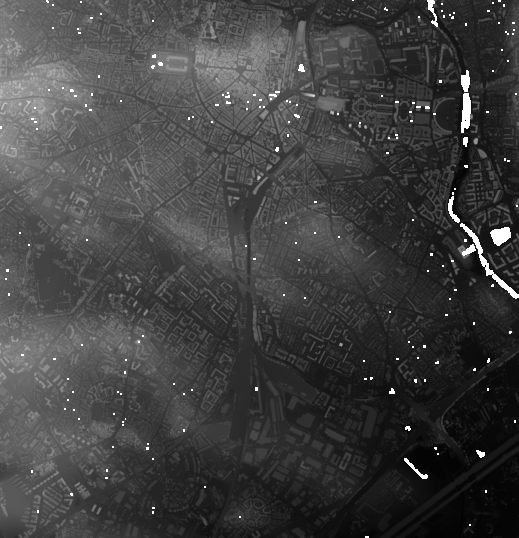
\includegraphics[width=\linewidth]{Images/Chap_6/miniature_Montpellier_gt.png}
        \caption{\acrshort{lidar} HD \acrshort{dsm}}
        \label{fig:miniature_Montpellier_gt}
    \end{subfigure}
    \caption{\acrshort{rgb} image of Montpellier and its associated ground truth \acrshort{dsm}.}
    \label{fig:miniature_Montpellier}
\end{figure}

\begin{figure}
    \centering
    \begin{subfigure}[t]{0.48\linewidth}
        \flushleft
        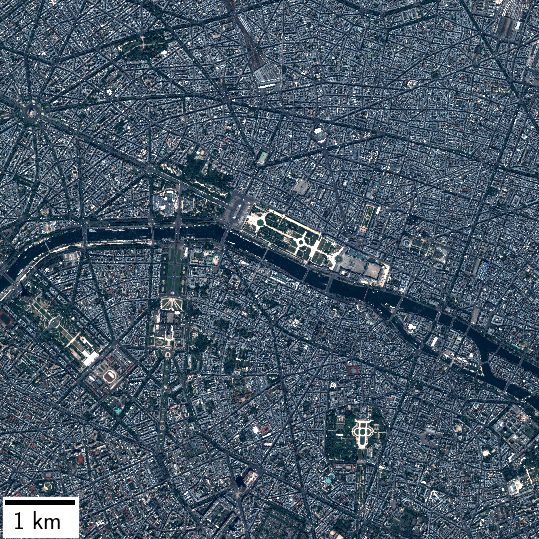
\includegraphics[width=\linewidth]{Images/Chap_6/miniature_Paris.png}
        \caption{\acrshort{rgb} image of Paris (Pléiades © \acrshort{cnes} 2023, Distribution AIRBUS DS)}
        \label{fig:miniature_Paris_rgb}
    \end{subfigure}\hfill
    \begin{subfigure}[t]{0.48\linewidth}
        \flushright
        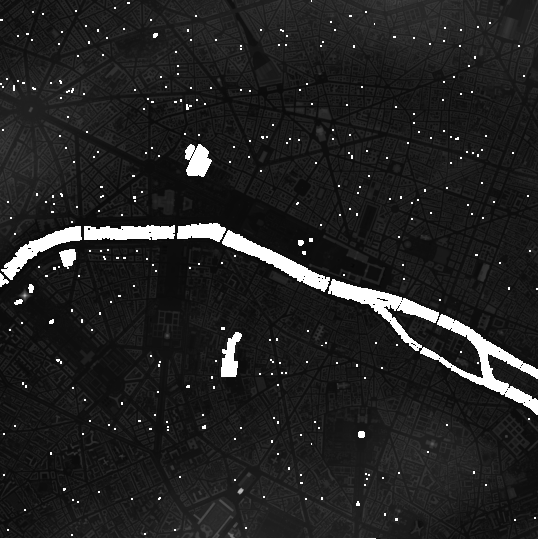
\includegraphics[width=\linewidth]{Images/Chap_6/miniature_Paris_gt.png}
        \caption{\acrshort{lidar} HD \acrshort{dsm}}
        \label{fig:miniature_Paris_gt}
    \end{subfigure}
    \caption{\acrshort{rgb} image of  and its associated ground truth \acrshort{dsm}.}
    \label{fig:miniature_Paris}
\end{figure}

\begin{figure}
    \centering
    \begin{subfigure}[t]{0.48\linewidth}
        \flushleft
        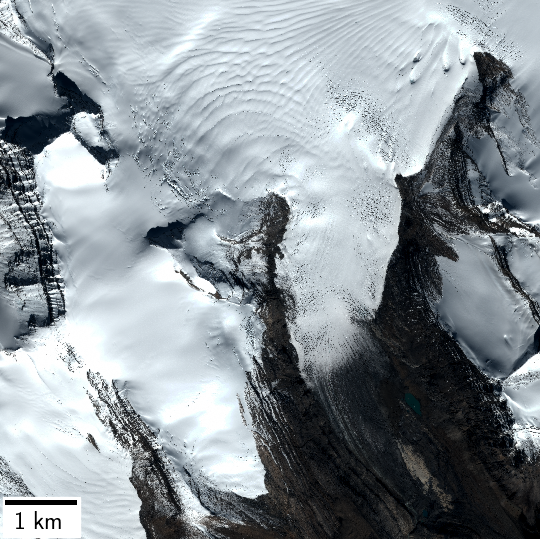
\includegraphics[width=\linewidth]{Images/Chap_6/miniature_Peyto.png}
        \caption{\acrshort{rgb} image of Peyto (Pléiades © \acrshort{cnes} 2016, Distribution AIRBUS DS)}
        \label{fig:miniature_Peyto_rgb}
    \end{subfigure}\hfill
    \begin{subfigure}[t]{0.48\linewidth}
        \flushright
        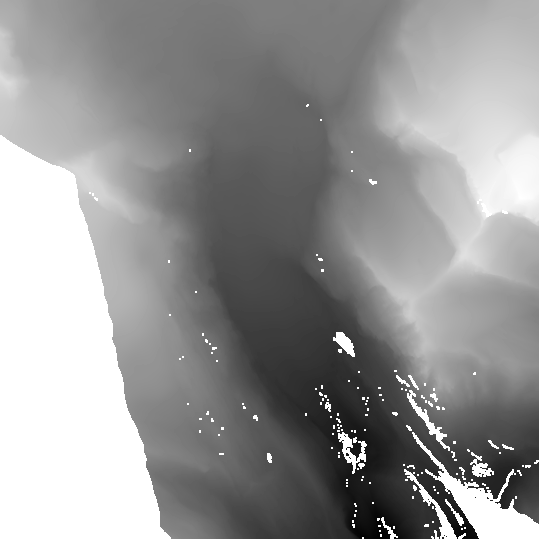
\includegraphics[width=\linewidth]{Images/Chap_6/miniature_Peyto_gt.png}
        \caption{\acrshort{lidar} HD \acrshort{dsm}}
        \label{fig:miniature_Peyto_gt}
    \end{subfigure}
    \caption{\acrshort{rgb} image of Peyto and its associated ground truth \acrshort{dsm}.}
    \label{fig:miniature_Peyto}
\end{figure}

\begin{figure}
    \centering
    \begin{subfigure}[t]{0.48\linewidth}
        \flushleft
        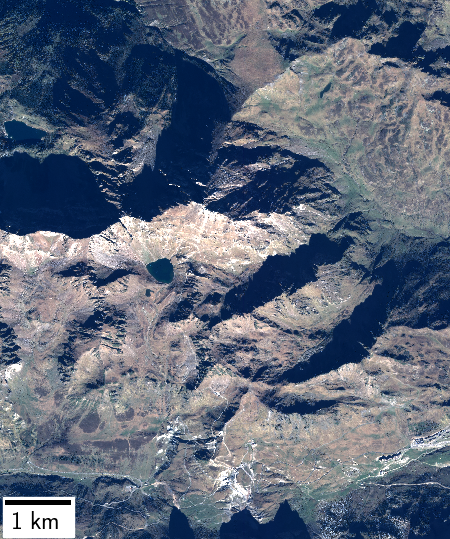
\includegraphics[width=\linewidth]{Images/Chap_6/miniature_Pic_du_midi.png}
        \caption{\acrshort{rgb} image of Pic du Midi (Pléiades © \acrshort{cnes} 2021, Distribution AIRBUS DS)}
        \label{fig:miniature_pic_du_midi_rgb}
    \end{subfigure}\hfill
    \begin{subfigure}[t]{0.48\linewidth}
        \flushright
        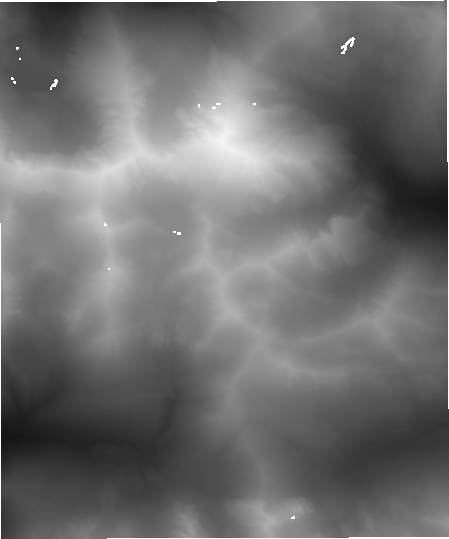
\includegraphics[width=\linewidth]{Images/Chap_6/miniature_Pic_du_midi_gt.png}
        \caption{\acrshort{lidar} HD \acrshort{dsm}}
        \label{fig:miniature_pic_du_midi_gt}
    \end{subfigure}
    \caption{\acrshort{rgb} image of Pic du Midi and its associated ground truth \acrshort{dsm}.}
    \label{fig:miniature_pic_du_midi}
\end{figure}

\begin{figure}
    \centering
    \begin{subfigure}[t]{0.48\linewidth}
        \flushleft
        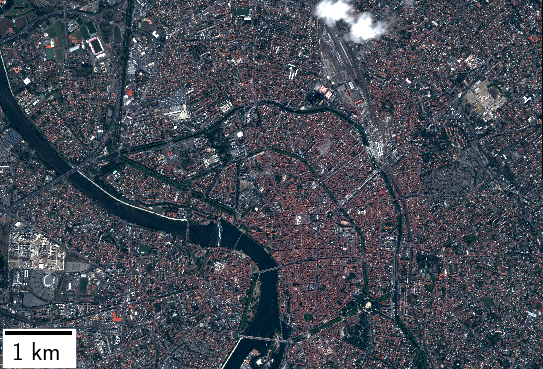
\includegraphics[width=\linewidth]{Images/Chap_6/miniature_Toulouse.png}
        \caption{\acrshort{rgb} image of Toulouse (Pléiades © \acrshort{cnes} 2022, Distribution AIRBUS DS)}
        \label{fig:miniature_Toulouse_rgb}
    \end{subfigure}\hfill
    \begin{subfigure}[t]{0.48\linewidth}
        \flushright
        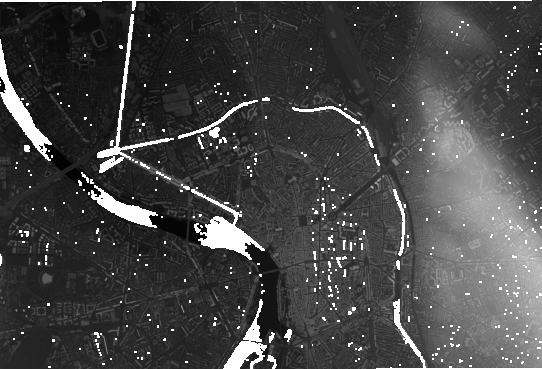
\includegraphics[width=\linewidth]{Images/Chap_6/miniature_Toulouse_gt.png}
        \caption{\acrshort{lidar} HD \acrshort{dsm}}
        \label{fig:miniature_Toulouse_gt}
    \end{subfigure}
    \caption{\acrshort{rgb} image of Toulouse and its associated ground truth \acrshort{dsm}.}
    \label{fig:miniature_Toulouse}
\end{figure}

\subsection{Water Masks}
Both \acrshort{lidar} data and stereo correlation present poor results on water surfaces. For the \acrshort{lidar} data, wavelengths are often absorbed by still water and do not provide the sensor with any feedback (although turbid water can usually send back some signal). For moving waters, the provided signal is often noisy and needs post-processing to remove artifacts. Stereophotogrammetry has usually even poorer results, because open waters are texture-less or uniform surfaces on which the correlation does not perform well. Furthermore, for Pléiades acquisitions, the water may have moved between images, which prevents water pixels from being correctly triangulated. For those reasons, we chose to add a water mask on images of cities crossed by a river (Bordeaux, Monaco, Montpellier, Paris, and Toulouse) or near the seaside (Monaco). The water mask was obtained using an algorithm developed by \acrshort{cnes}, which uses a random forest trained on existing high resolution mapping of surface waters \cite{pekel_high-resolution_2016} and the Normalized Difference Water Index \cite{gao_ndwinormalized_1996}. \Cref{fig:paris_watermask_2} presents a water mask produced on the image of Paris.

\begin{figure}
    \centering
    \begin{subfigure}[t]{0.48\linewidth}
        \flushleft
        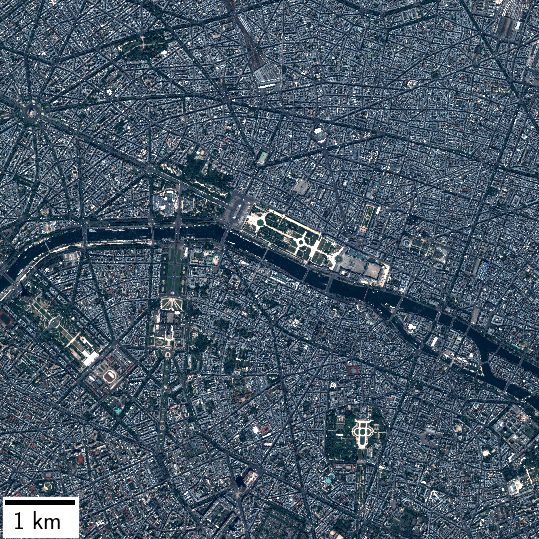
\includegraphics[width=\linewidth]{Images/Chap_6/miniature_Paris.png}
        \caption{\acrshort{rgb} image of Paris (Pléiades © \acrshort{cnes} 2023, Distribution AIRBUS DS)}
        \label{fig:paris_watermask_1}
    \end{subfigure}\hfill
    \begin{subfigure}[t]{0.48\linewidth}
        \flushright
        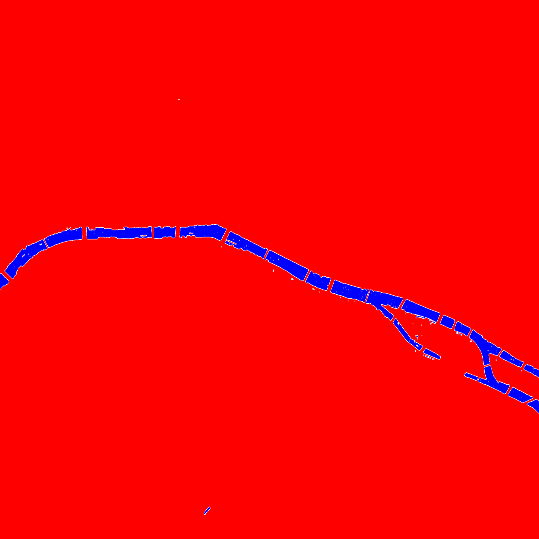
\includegraphics[width=\linewidth]{Images/Chap_6/watermask_Paris.png}
        \caption{Water mask}
        \label{fig:paris_watermask_2}
    \end{subfigure}
    \caption{\acrshort{rgb} image of Paris and its associated water mask. Water is indicated by blue pixels}
    \label{fig:paris_watermask}
\end{figure}

\subsection{Co-registration}
The \acrshort{dsm}s obtained from \acrshort{lidar} data and from stereophotogrammetry are not necessarily in the same projection reference system, and do not use the same altitude reference. Moreover, due to the limited accuracy of \acrshort{rpc} models and GPS measures of the \acrshort{lidar}, some planimetric and elevation biases may exist between the two \acrshort{dsm}s. Those biases do not allow their comparison as such. We therefore reproject the ground truth data in the same reference system as their corresponding \acrshort{dsm} produced by the CARS pipeline. We then rectify the planimetric and altimetric biases by applying the method presented in \cite{nuth_co-registration_2011}. This process is called co-registration. We quickly present the method for estimating the altimetric and planimetric biases, and refer to the original publication for additional details.

It is possible to observe that the measured differences between two shifted \acrshort{dsm}s vary with the slope angle and the orientation of the slope. The different parameters influencing the measured variations of elevation, presented in \Cref{fig:coregistration}, are the following:
\begin{itemize}
    \item We note $sl$ the angle of a slope. $sl=0\degree$ corresponds to a flat slope and $sl=90\degree$ to a vertical slope.
    \item We note $\psi$ the azimuth of the slope. If the slope faces north, then $\psi=0\degree$. If it faces west, $\psi=90\degree$ \etc
    \item The direction of the planimetric shift between \acrshort{dsm}s is given by an angle $\beta$, with the same conventions as the azimuth. The magnitude of the shift is $B$.
    \item $dh$ refers to measured local variations of elevation, and $\tilde{dh}$ is the global elevation shift between \acrshort{dsm}s.
\end{itemize}
The relation linking all those parameters is the following \cite{nuth_co-registration_2011}:
\begin{align}
    dh = B\cos(\psi-\beta)\tan(sl)+\tilde{dh}
\end{align}

\begin{figure}[ht!]
    \centering
    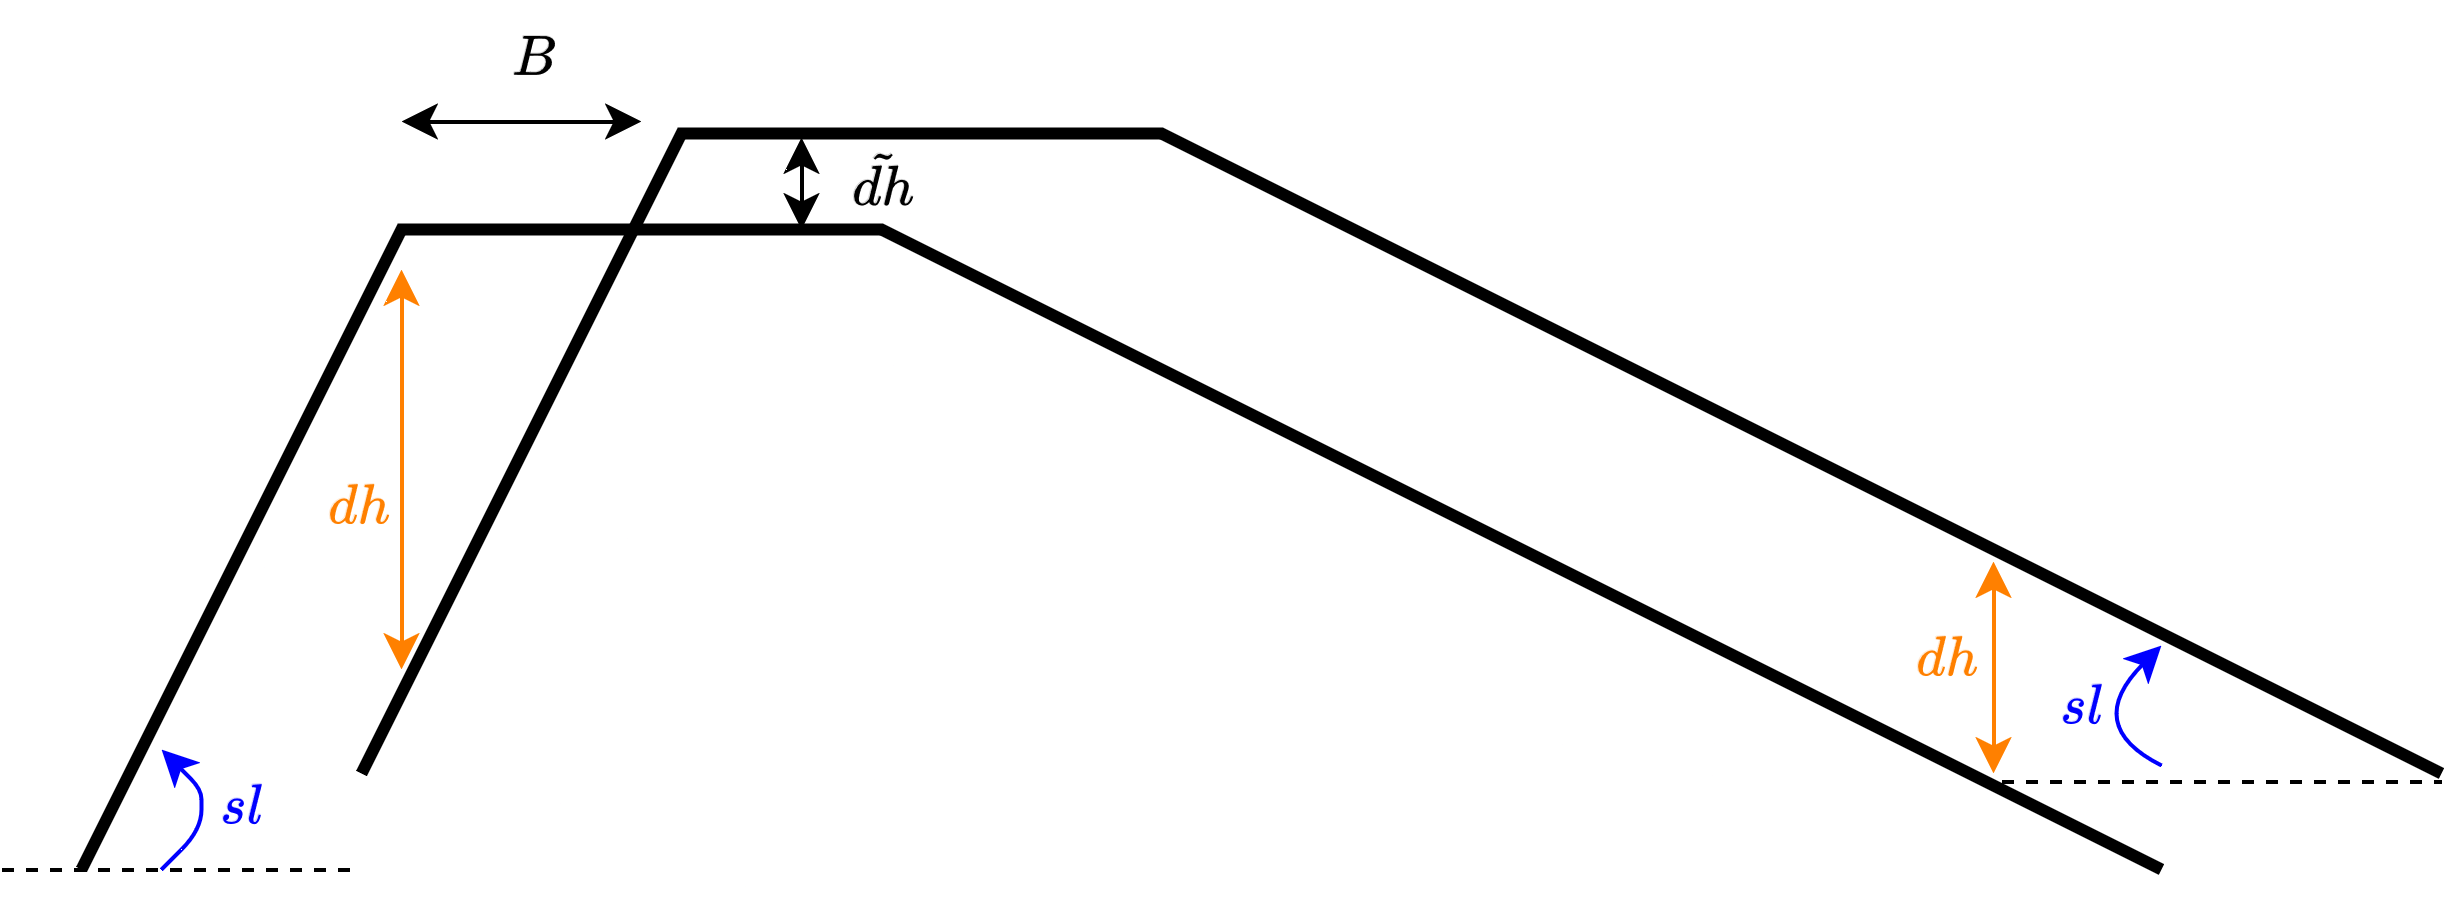
\includegraphics[width=\linewidth]{Images/Chap_6/Coregistration.png}
    \caption{Planimetric shift of magnitude $B$ and altimetric shift $\tilde{dh}$ between two \acrshort{dsm}s. We can see that local variations $\tilde{dh}$ vary depending on the slope $sl$. This diagram is in 2D, the angle of the planimetric shift and the azimuth of the slope are therefore not represented.}
    \label{fig:coregistration}
\end{figure}

The three unknowns are $B$, $\beta$ and $\tilde{dh}$, as the slope parameters can be computed by any \acrshort{gis} software from the \acrshort{dsm}s. For instance, the slope of $\DSM_{true}$ is computed as:
\begin{align}\label{eq:slope}
    sl(x,y) = \dfrac{1}{8}\sqrt{\left(\dfrac{\DSM_{true}\ast k_x(x,y)}{r_x}\right)^2 + \left(\dfrac{\DSM_{true}\ast k_y(x,y)}{r_y}\right)^2}
\end{align}
where $\ast$ denotes a convolution with two kernels $k_x=\begin{bmatrix}
-1 & 0 & 1\\
-2 & 0 & 2 \\
-1 & 0 & 1
\end{bmatrix}$, $k_y=\begin{bmatrix}
-1 & -2 & -1\\
0 & 0 & 0 \\
1 & 2 & 1
\end{bmatrix}$, and $r_x$, $r_y$ are the resolution in $x$ and $y$. We will use the slope in the evaluation of the different metrics.

The unknowns $B$, $\beta$ and $\tilde{dh}$ are determined by a least square optimization problem. Because the \acrshort{dsm} is not expressed analytically, the optimization is not guaranteed to be exact. Multiple iterations of the planimetric and altimetric shift estimation lead to a better final result. An illustration of the co-registration process is presented in \Cref{fig:coregistration_image}.

The problem we encounter is that the \acrshort{dsm} obtained from photogrammetry already possess some errors. In the least squared minimization problem, the residuals computed from the difference between the ground truth \acrshort{dsm} and the photogrammetry \acrshort{dsm} therefore also contain those errors. This deteriorates the quality of the co-registration. However, it remains the best solution for co-registering \acrshort{dsm}s. We apply this co-registration to our data, before computing any metric. The different metrics we consider will be presented in \Cref{sec:metrics_elevation}, while the following sections details the parameters used in our stereo pipeline.

\begin{figure}
    \centering
    \begin{subfigure}[t]{0.48\linewidth}
        \centering
        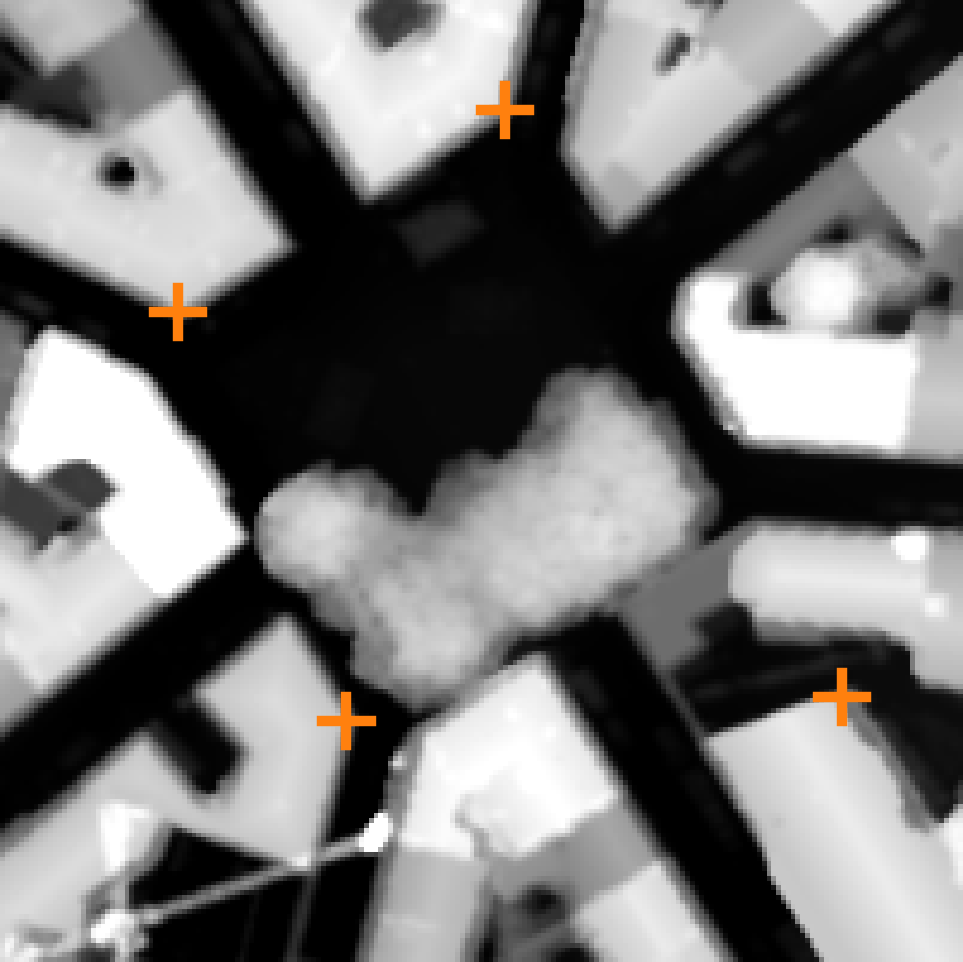
\includegraphics[width=\linewidth]{Images/Chap_6/coregisration_planimetric_shift_gt_toulouse.png}
        \caption{Ground Truth \acrshort{dsm}}
        \label{fig:coregistration_planimetric_gt}
    \end{subfigure}\hfill
    \begin{subfigure}[t]{0.48\linewidth}
        \flushright
        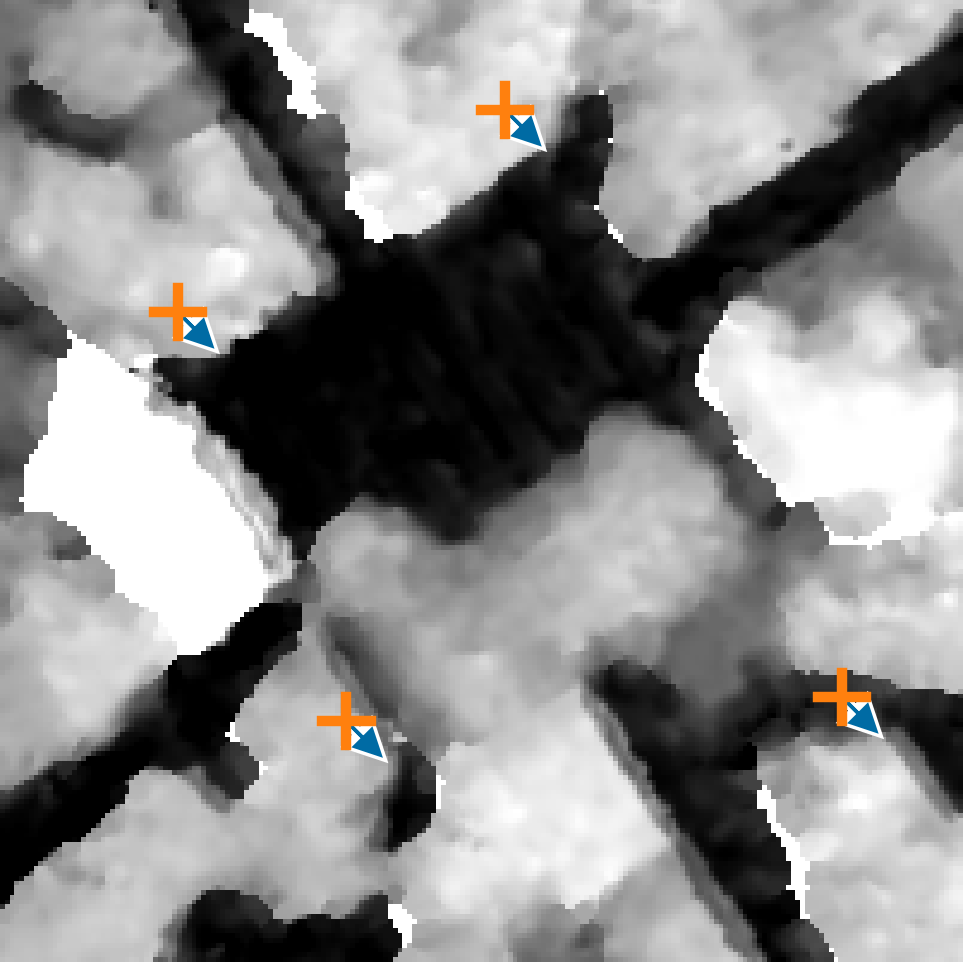
\includegraphics[width=\linewidth]{Images/Chap_6/coregisration_planimetric_shift_cars_toulouse.png}
        \caption{CARS \acrshort{dsm}}
        \label{fig:coregistration_planimetric_cars}
    \end{subfigure}\\
    \begin{subfigure}[t]{\linewidth}
        \centering
        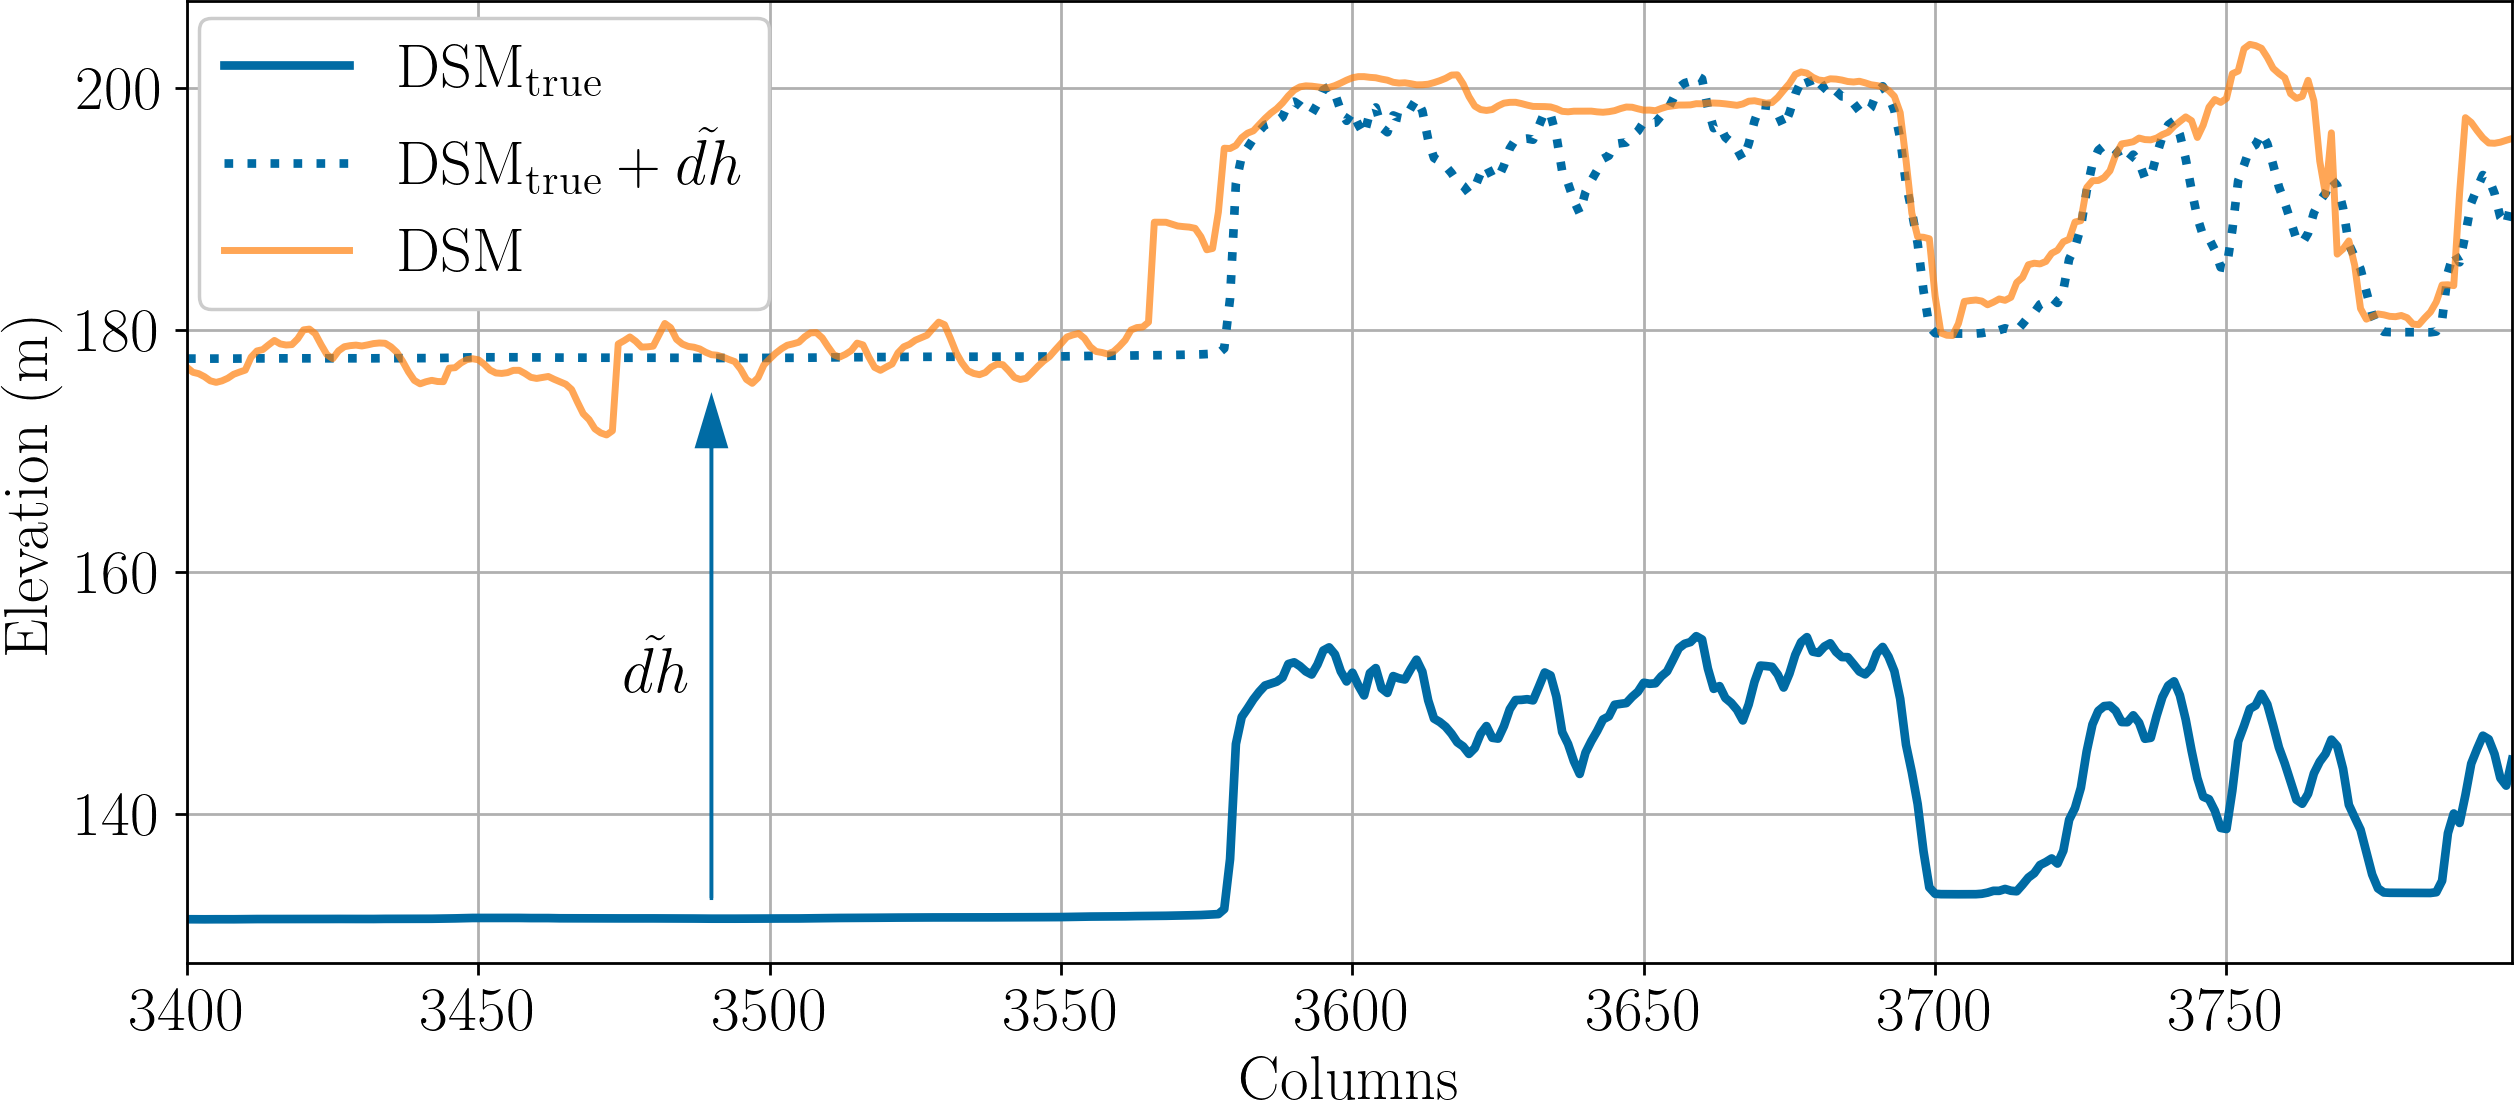
\includegraphics[width=\linewidth]{Images/Chap_6/coregisration_altimetric_shift_toulouse.png}
        \caption{Elevation along a row of the \acrshort{dsm}}
        \label{fig:coregistration_altimetric}
    \end{subfigure}
    \caption{Planimetric shift and altimetric shift from the co-registration step over the city of Toulouse. In \subref{fig:coregistration_planimetric_gt} and \subref{fig:coregistration_planimetric_cars}, reference points in orange are located at the same row and columns in the two \acrshort{dsm}s. The planimetric shift is indicated with blue arrows. \subref{fig:coregistration_altimetric} presents the altimetric shift between the two \acrshort{dsm}s.}
    \label{fig:coregistration_image}
\end{figure}

\subsection{Configuration of the Photogrammetry Pipeline}
This section provides technical information about the configuration of the CARS pipeline used to process the satellite images.

We used the Copernicus DEM with a 30m resolution as the reference altitude, as the SRTM elevation models were not available for high latitudes, such as Norway for instance. We used the same range of considered disparity for every image: [-50pix, 50pix]. This range is quite high, especially for acquisition with a high altitude ratio $r_{alt}$, but ensures we are not limited to a restrictive range of possible elevations.

Although we developed a method for creating disparity intervals which works for both the CENSUS and MC-CNN cost functions, we will only present results using the CENSUS cost function. Two reasons motivate this choice. First, due to the quantity of scenes and the variety of analyses completed, it would quickly become quite overwhelming to present each result for both cost functions, especially when there is no major difference between the two. Secondly, we observed in the previous chapter that disparity intervals obtained using CENSUS were less accurate than those using MC-CNN. As we favor accuracy above interval size, we chose to use the CENSUS cost function throughout our results, as validating the accuracy requirements for CENSUS ensures that they are also validated using MC-CNN. We verified that there was no unexpected behavior for MC-CNN intervals across scenes, and since nothing notable appeared, we did not delve into so many details as we did for the CENSUS intervals.  

We detail here the list of the parameters used in the pipeline. The CENSUS cost function was computed using a 5$\times$5 window. The \acrshort{sgm} penalties used for regularizing the CENSUS cost volume were $P_1=8$ and $P_2=32$. Disparity intervals were produced using a possibility threshold of $0.9$. Intervals were regularized in low confidence areas for which the confidence from ambiguity was below $0.6$, after being minimized by a minitive kernel of shape $(1, 2\cdot k_{amb}+1)=(1,5)$. For each regularized pixel, we took the $90$\ith upper and $10$\ith lower quantiles over a low confidence area that extended $n_\N=3$ rows above and below. A V-fit refinement step was used to get sub-pixel disparities, and a median filter of shape $(3\times 3)$ was applied to the resulting disparity map. Pixels that did not validate the cross-checking criterion from \Cref{eq:cross-checking} were not considered for triangulation. Triangulated 3D points were filtered using \Cref{eq:statistical_outlier} with $k=5$ and $N=50$, and \Cref{eq:small_components} with $D_{max}=3$ m and $N_{min}=50$. The rasterization from \Cref{eq:rasterization} used $\sigma=0.3$ m and $r=3$ m.

\section{Metrics for Evaluating Elevation Intervals}\label{sec:metrics_elevation}
We introduce here the metrics used to evaluate the performance of elevation intervals. In order to stay consistent with \Cref{sec:metrics_disparity}, we consider the metrics introduced for disparity intervals and adapt them to elevation intervals. 

We will refer to the true elevation as $\DSM_{true}$, the predicted elevation as $\DSM$ and the elevation intervals as $[\underline{\DSM},~\overline{\DSM}]$.

\subsubsection{Elevation Accuracy Metric}
Similarly to \Cref{sec:metrics_disparity}, the first metric is the proportion of correct intervals, \ie the proportion of intervals containing the ground truth. We call this metric the elevation accuracy $Z_{acc}$:
\begin{align}\label{eq:relative_accuracy_elevation}
    Z_{acc} = \dfrac{\#\{\DSM_{true} ~|~ \st ~\DSM_{true}\in [\underline{\DSM},~\overline{\DSM}]\}}{\#\{\DSM_{true}\}}
\end{align}
\Cref{fig:Intervals_elevation_metrics_Z_acc} illustrates what this metric represents. $Z_{acc}$ is similar to $acc$ defined in \Cref{eq:accuracy} from \Cref{sec:metrics_disparity}, we thus want to maximize $Z_{acc}$. We also keep the objective of $90\%$ accuracy for our method, which was validated for the disparity intervals.

\begin{figure}
    \centering
    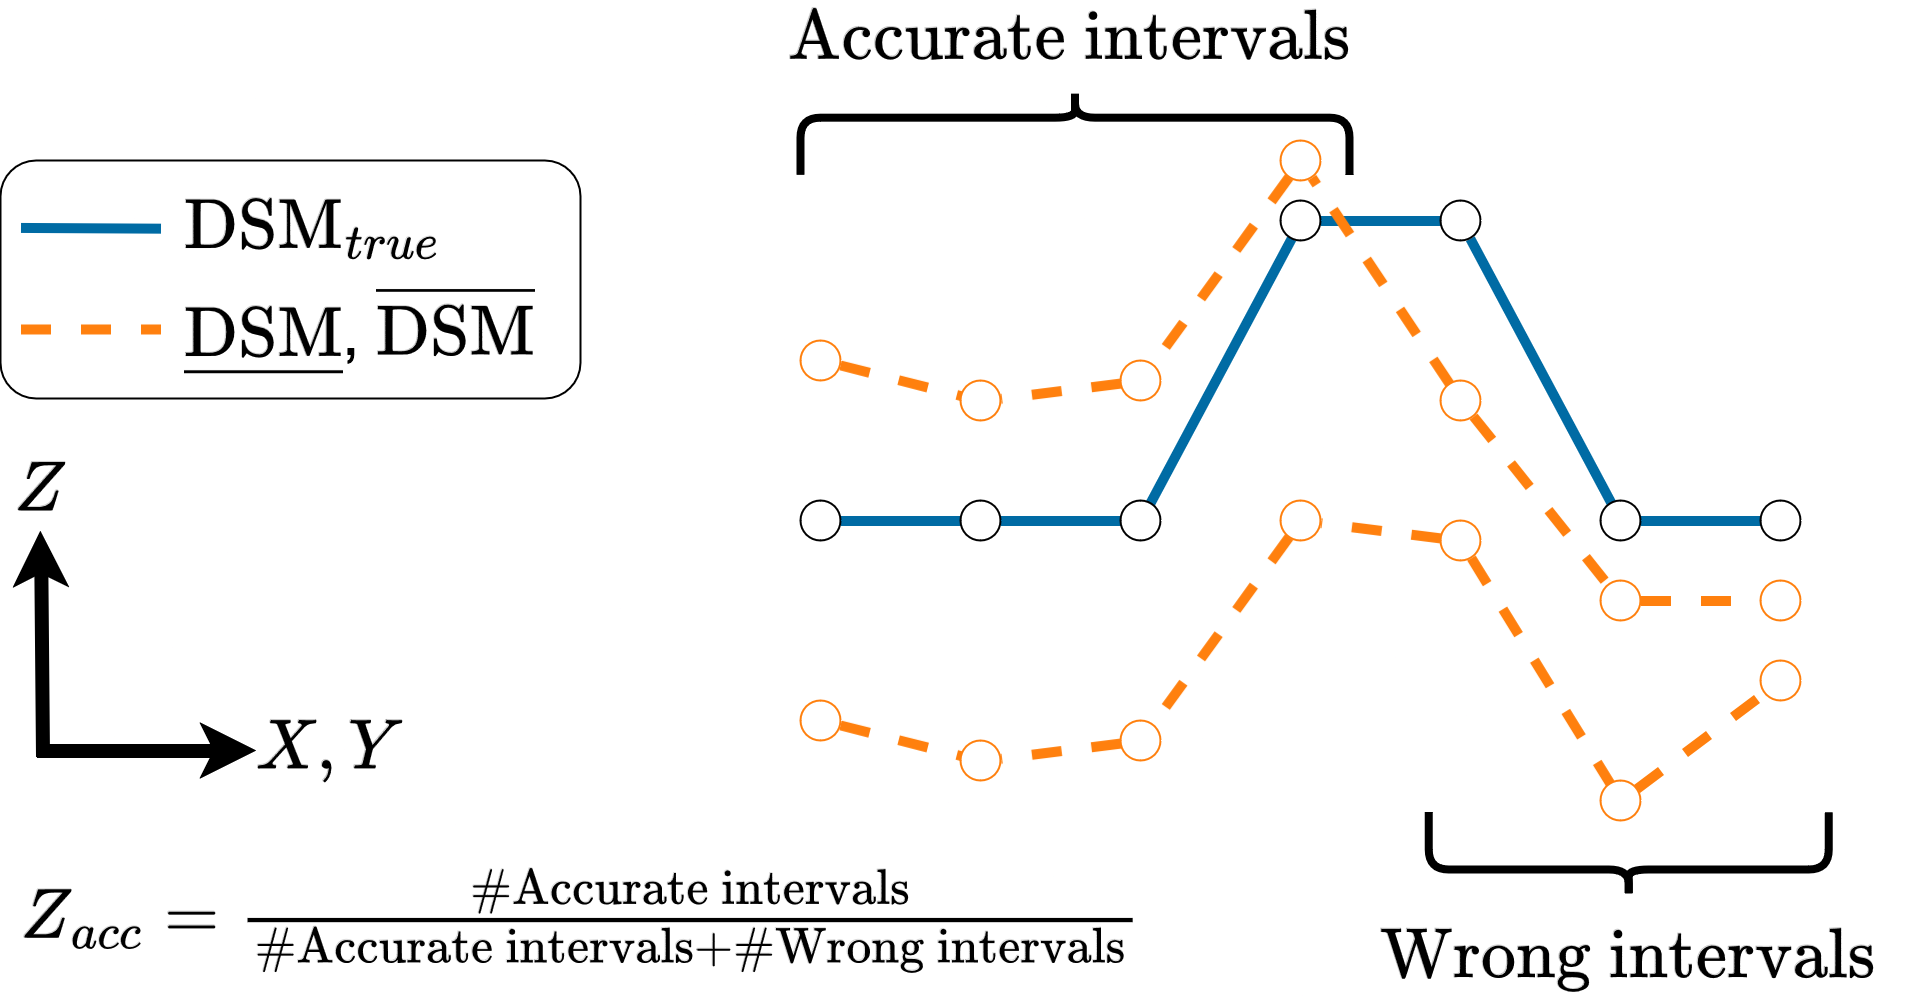
\includegraphics[width=0.7\linewidth]{Images/Chap_6/Intervals_elevation_metrics_Z_acc.png}
    \caption{Schematic representation of $Z_{acc}$}
    \label{fig:Intervals_elevation_metrics_Z_acc}
\end{figure}

\subsubsection{Residual Elevation Error Metric}
We are also interested in evaluating the magnitude of the errors. We thus define the residual elevation error $Z_{\varepsilon}$ for all intervals that do not contain the ground truth as:
\begin{align}
    Z_\varepsilon=\dfrac{1}{r_{alt}} \cdot\median \left( \min(|\DSM_{true}-\overline{\DSM}, ~ |\DSM_{true}-\underline{\DSM}|)\right)\label{eq:residual_error_elevation}
\end{align}
where $r_{alt}$ is the disparity to altitude ratio (or altimetric ratio), \ie the elevation difference resulting from a shift of one disparity. \Cref{fig:Intervals_elevation_metrics_Z_eps} illustrates what this metric represents. We want $Z_\varepsilon$ error to be as close to 0 as possible. $r_{alt}$ has been computed alongside the epipolar grids (\Cref{sec:epipolar_geometry}). Dividing by the ratio $r_{alt}$ effectively converts $\min(|\DSM_{true}-\overline{\DSM}|, |\DSM_{true}-\underline{\DSM}|)$ from meters to pixels. As an error of one disparity pixel in the dense matching step can result in an elevation error of 1m in a scene, and 2m in another, we divide by $r_{alt}$ in order to be able to compare stereo pairs with different convergence angles. \Cref{tab:elevation_metrics_global} contains the different altimetric ratios for the data we consider. $Z_{\varepsilon}$ is similar to $\varepsilon$ defined in \Cref{eq:residual_error} from \Cref{sec:metrics_disparity}.

\begin{figure}
    \centering
    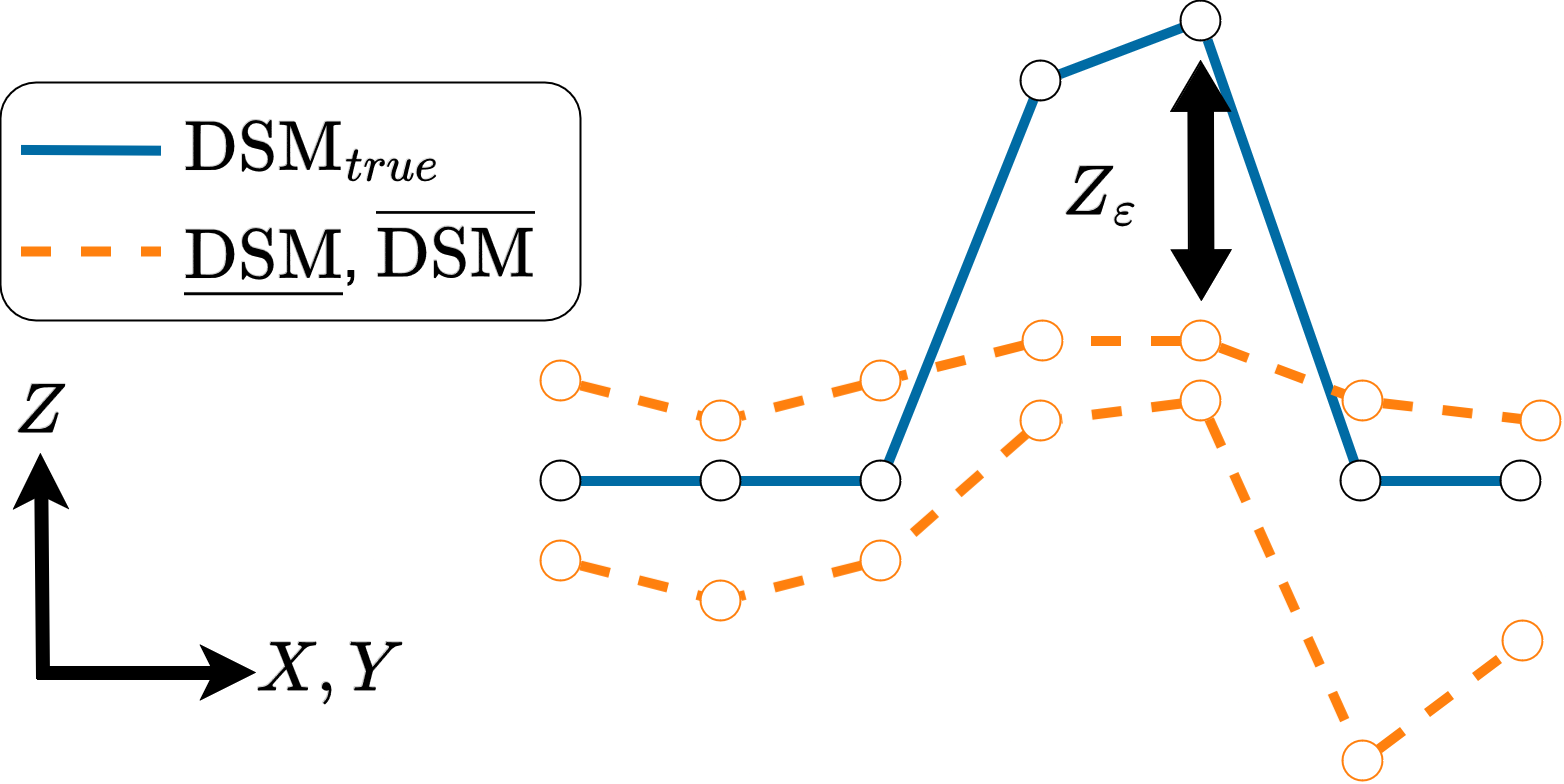
\includegraphics[width=0.7\linewidth]{Images/Chap_6/Intervals_elevation_metrics_Z_eps.png}
    \caption{Schematic diagram of the quantity represented by $Z_{\varepsilon}$}
    \label{fig:Intervals_elevation_metrics_Z_eps}
\end{figure}

\subsubsection{Relative Elevation Size Metric}
Those two previous metrics allow measuring the accuracy and errors of elevation intervals. To evaluate the size of intervals, we use the relative elevation size $Z_{size}$ defined as :
\begin{align}\label{eq:relative_size_elevation}
    Z_{size} = \dfrac{1}{r_{alt}}\median\left(\overline{\DSM}-\underline{\DSM}\right)
\end{align}
We divide by the altimetric ratio for the same reasons as in $Z_\varepsilon$, \ie to compare stereo pairs with different convergence angles. \Cref{fig:Intervals_elevation_metrics_Z_size} illustrates what this metric represents. We want the relative elevation size to be as close to zero as possible. $Z_{size}$ is similar to $s_{rel}$ defined in \Cref{eq:relative_size_disparity} from \Cref{sec:metrics_disparity}.

\begin{figure}
    \centering
    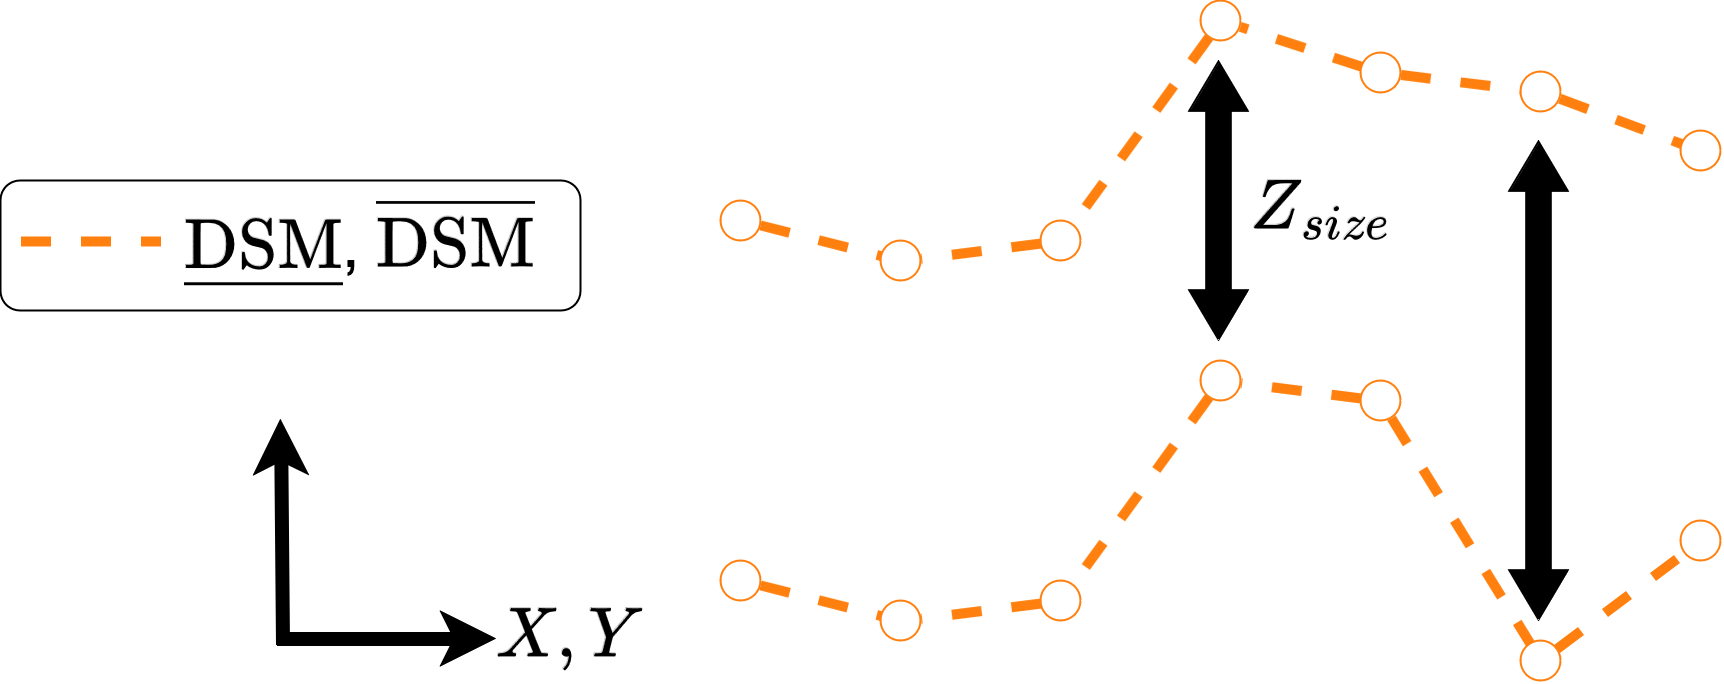
\includegraphics[width=0.7\linewidth]{Images/Chap_6/Intervals_elevation_metrics_Z_size.png}
    \caption{Schematic diagram of the quantity represented by $Z_{size}$}
    \label{fig:Intervals_elevation_metrics_Z_size}
\end{figure}

\begin{remark}
    In the rasterization process, 3D points from low confidence area are mixed with points from high confidence areas. We therefore are unable to define interval regularization areas in the final \acrshort{dsm}. The relative over-estimation $o_{rel}$ has therefore no equivalent for elevation intervals.  
\end{remark}

\section{Elevation Intervals Results}\label{sec:results_elevation}
\begin{table}[ht]
    \centering
    \begin{tabular}{|c||c|c|c|c|c|c|}
        \hline
        Scene & $Z_{acc}$ & $Z_\varepsilon$ (pix) & $Z_{size}$ (pix) & $r_{alt}$ (m/pix) & invalid
        \\\hline\hline
        Bordeaux & 89.3$\%$ & 0.56 & 4.18 & 1.24  & 21.5$\%$\\\hline
        Graasubreen & 99.7$\%$ & 0.12 & 1.96 & 1.32  & 27.5$\%$\\\hline
        Hellmem & 98.8$\%$ & 2.76 & 2.02 & 1.32  & 34.7$\%$\\\hline
        Grenoble & 93.1$\%$ & 0.87 & 3.99 & 1.06  & 6.4$\%$\\\hline
        Langfjordjøkelen & 99.4$\%$ & 0.30 & 2.16 & 1.35  & 13.9$\%$\\\hline
        Monaco & 90.3$\%$ & 0.57 & 3.76 & 0.99  & 41.9$\%$\\\hline
        Montpellier & 89.1$\%$ & 0.28 & 2.05 & 3.64  & 1.9$\%$\\\hline
        Paris & 84.6$\%$ & 0.46 & 2.01 & 5.78  & 3.0$\%$\\\hline
        Peyto & 98.9$\%$ & 0.18 & 2.08 & 1.66  & 18.3$\%$\\\hline
        Pic du midi & 98.1$\%$ & 0.20 & 2.41 & 1.01  & 7.5$\%$\\\hline
        Toulouse & 92.0$\%$ & 0.38 & 2.04 & 2.43  & 6.9$\%$\\\hline
    \end{tabular}
    \caption{Elevation metrics for the different stereo pairs. The last column indicates the proportion of invalid pixels in the considered \acrshort{dsm}s.}
    \label{tab:elevation_metrics_global}
\end{table}

\begin{figure}
    \begin{subfigure}[t]{0.553\linewidth}
        \flushleft
        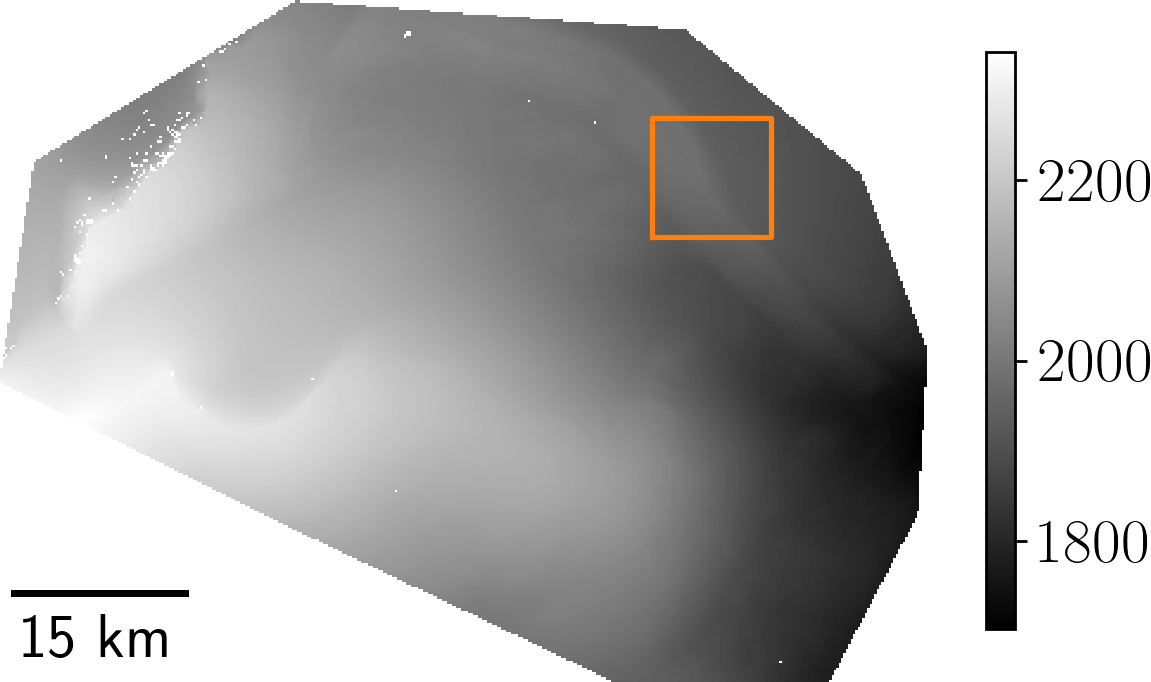
\includegraphics[width=\linewidth]{Images/Chap_6/Graasubreen_dsm.png}
        \caption{Photogrammetry \acrshort{dsm}. Orange area is detailed in \Cref{fig:Graasubreen_zoom}}
        \label{fig:Graasubreen_dsm}
    \end{subfigure}
    \begin{subfigure}[t]{0.447\linewidth}
        \flushright
        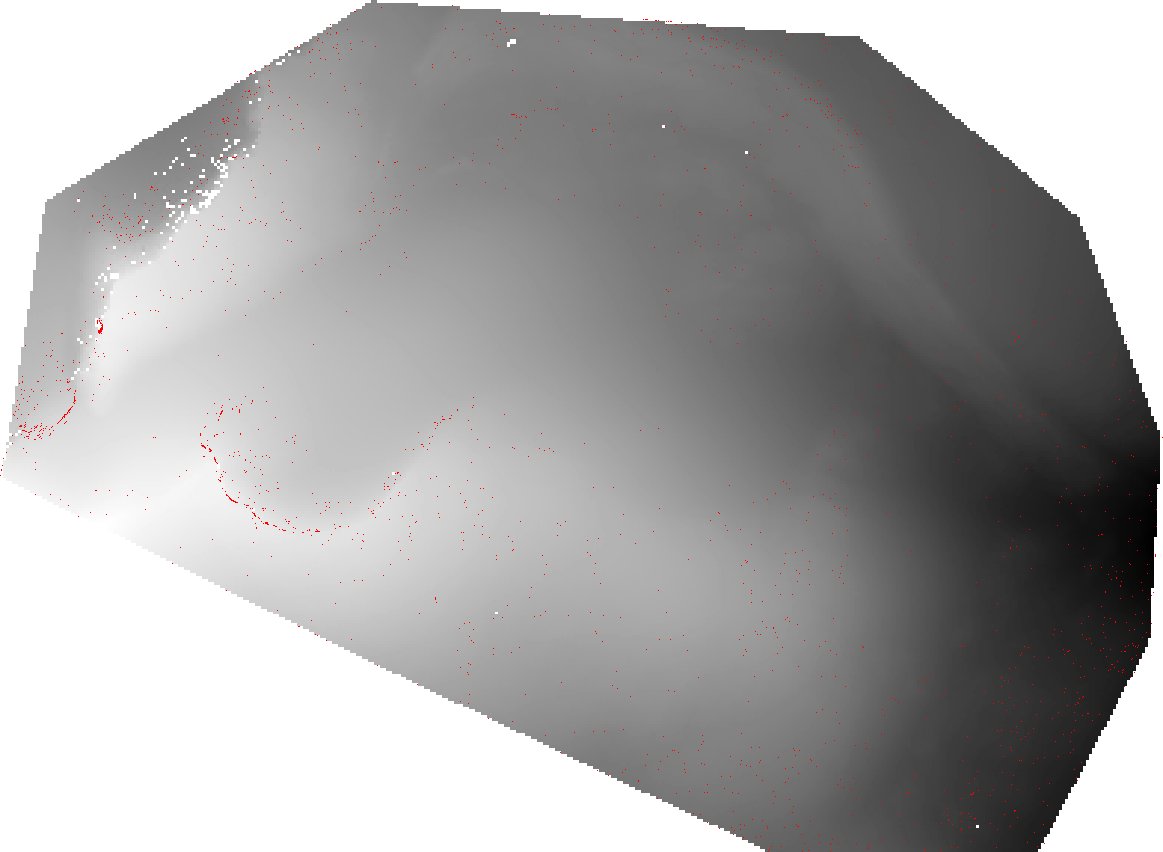
\includegraphics[width=\linewidth]{Images/Chap_6/Graasubreen_error.png}
        \caption{\acrshort{dsm} with wrong intervals in red.}
        \label{fig:Graasubreen_error}
    \end{subfigure}
    \caption{\acrshort{dsm} without and with wrong intervals over Graasubreen scene}
    \label{fig:Graasubreen_global}
\end{figure}

\begin{figure}
    \begin{subfigure}[t]{0.49\linewidth}
        \flushleft
        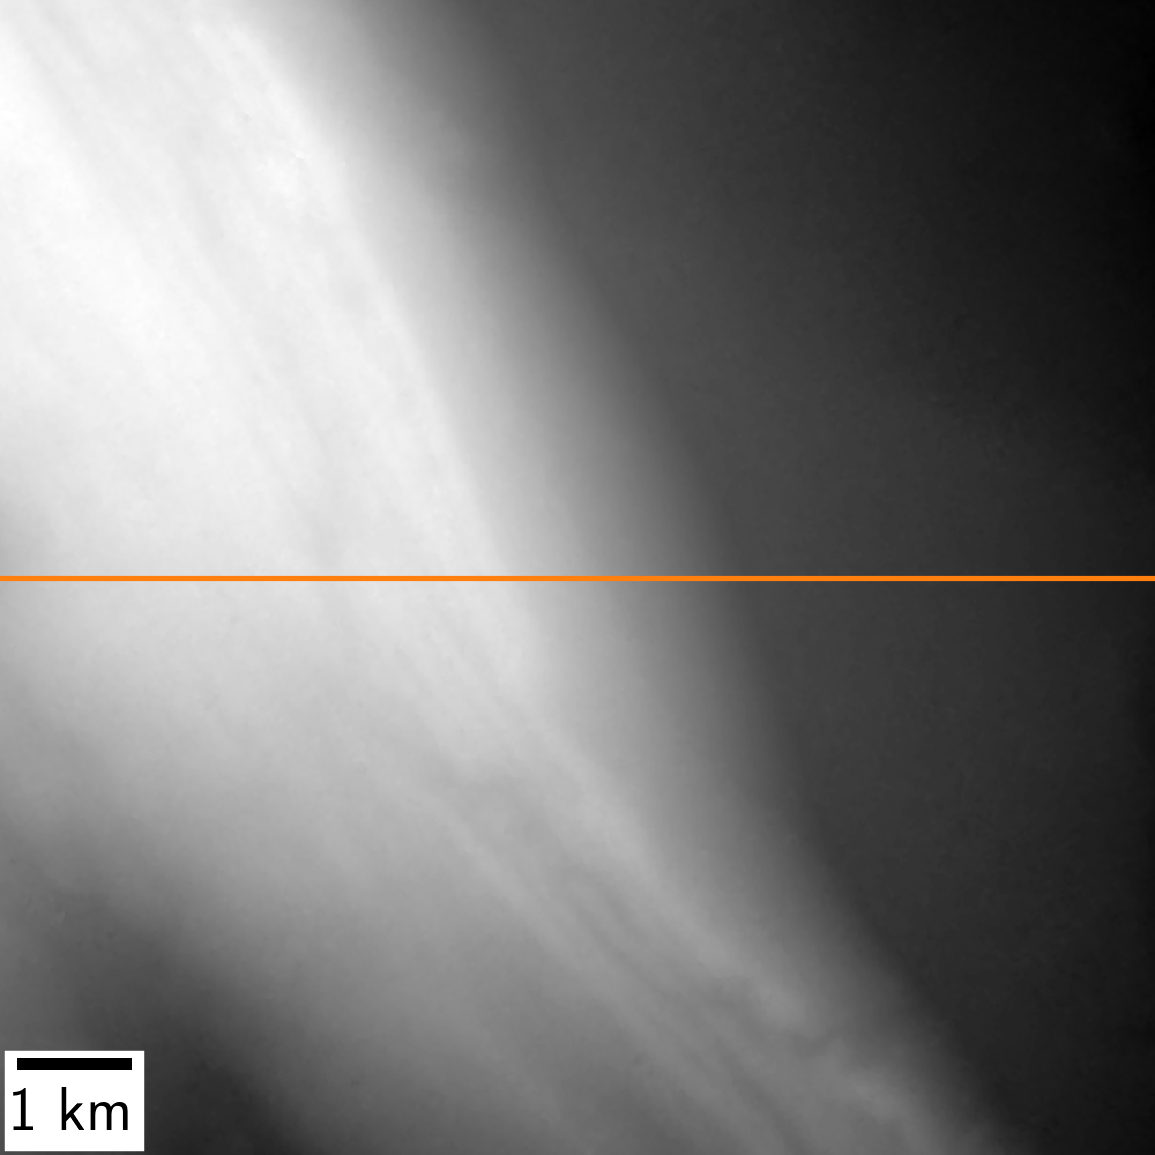
\includegraphics[width=\linewidth]{Images/Chap_6/Graasubreen_dsm_zoom.png}
        \caption{Photogrammetry \acrshort{dsm}. Orange line is detailed in \subref{fig:Graasubreen_zoom_row}}
        \label{fig:Graasubreen_dsm_zoom}
    \end{subfigure}\hfill
    \begin{subfigure}[t]{0.49\linewidth}
        \flushright
        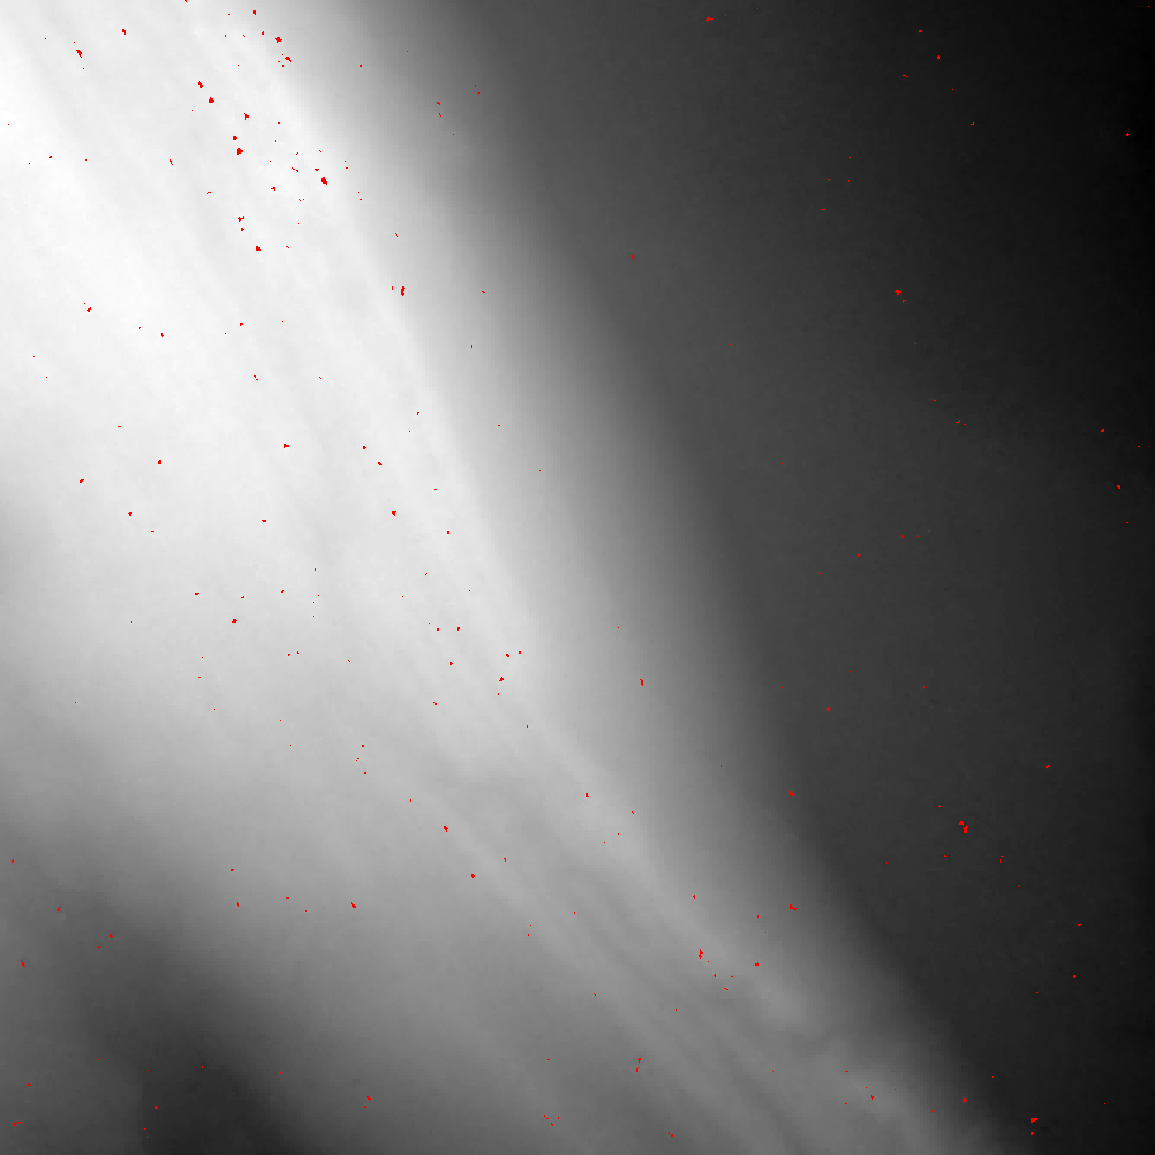
\includegraphics[width=\linewidth]{Images/Chap_6/Graasubreen_error_zoom.png}
        \caption{\acrshort{dsm} with wrong intervals in red.}
        \label{fig:Graasubreen_error_zoom}
    \end{subfigure}
    \begin{subfigure}[t]{\linewidth}
        \centering
        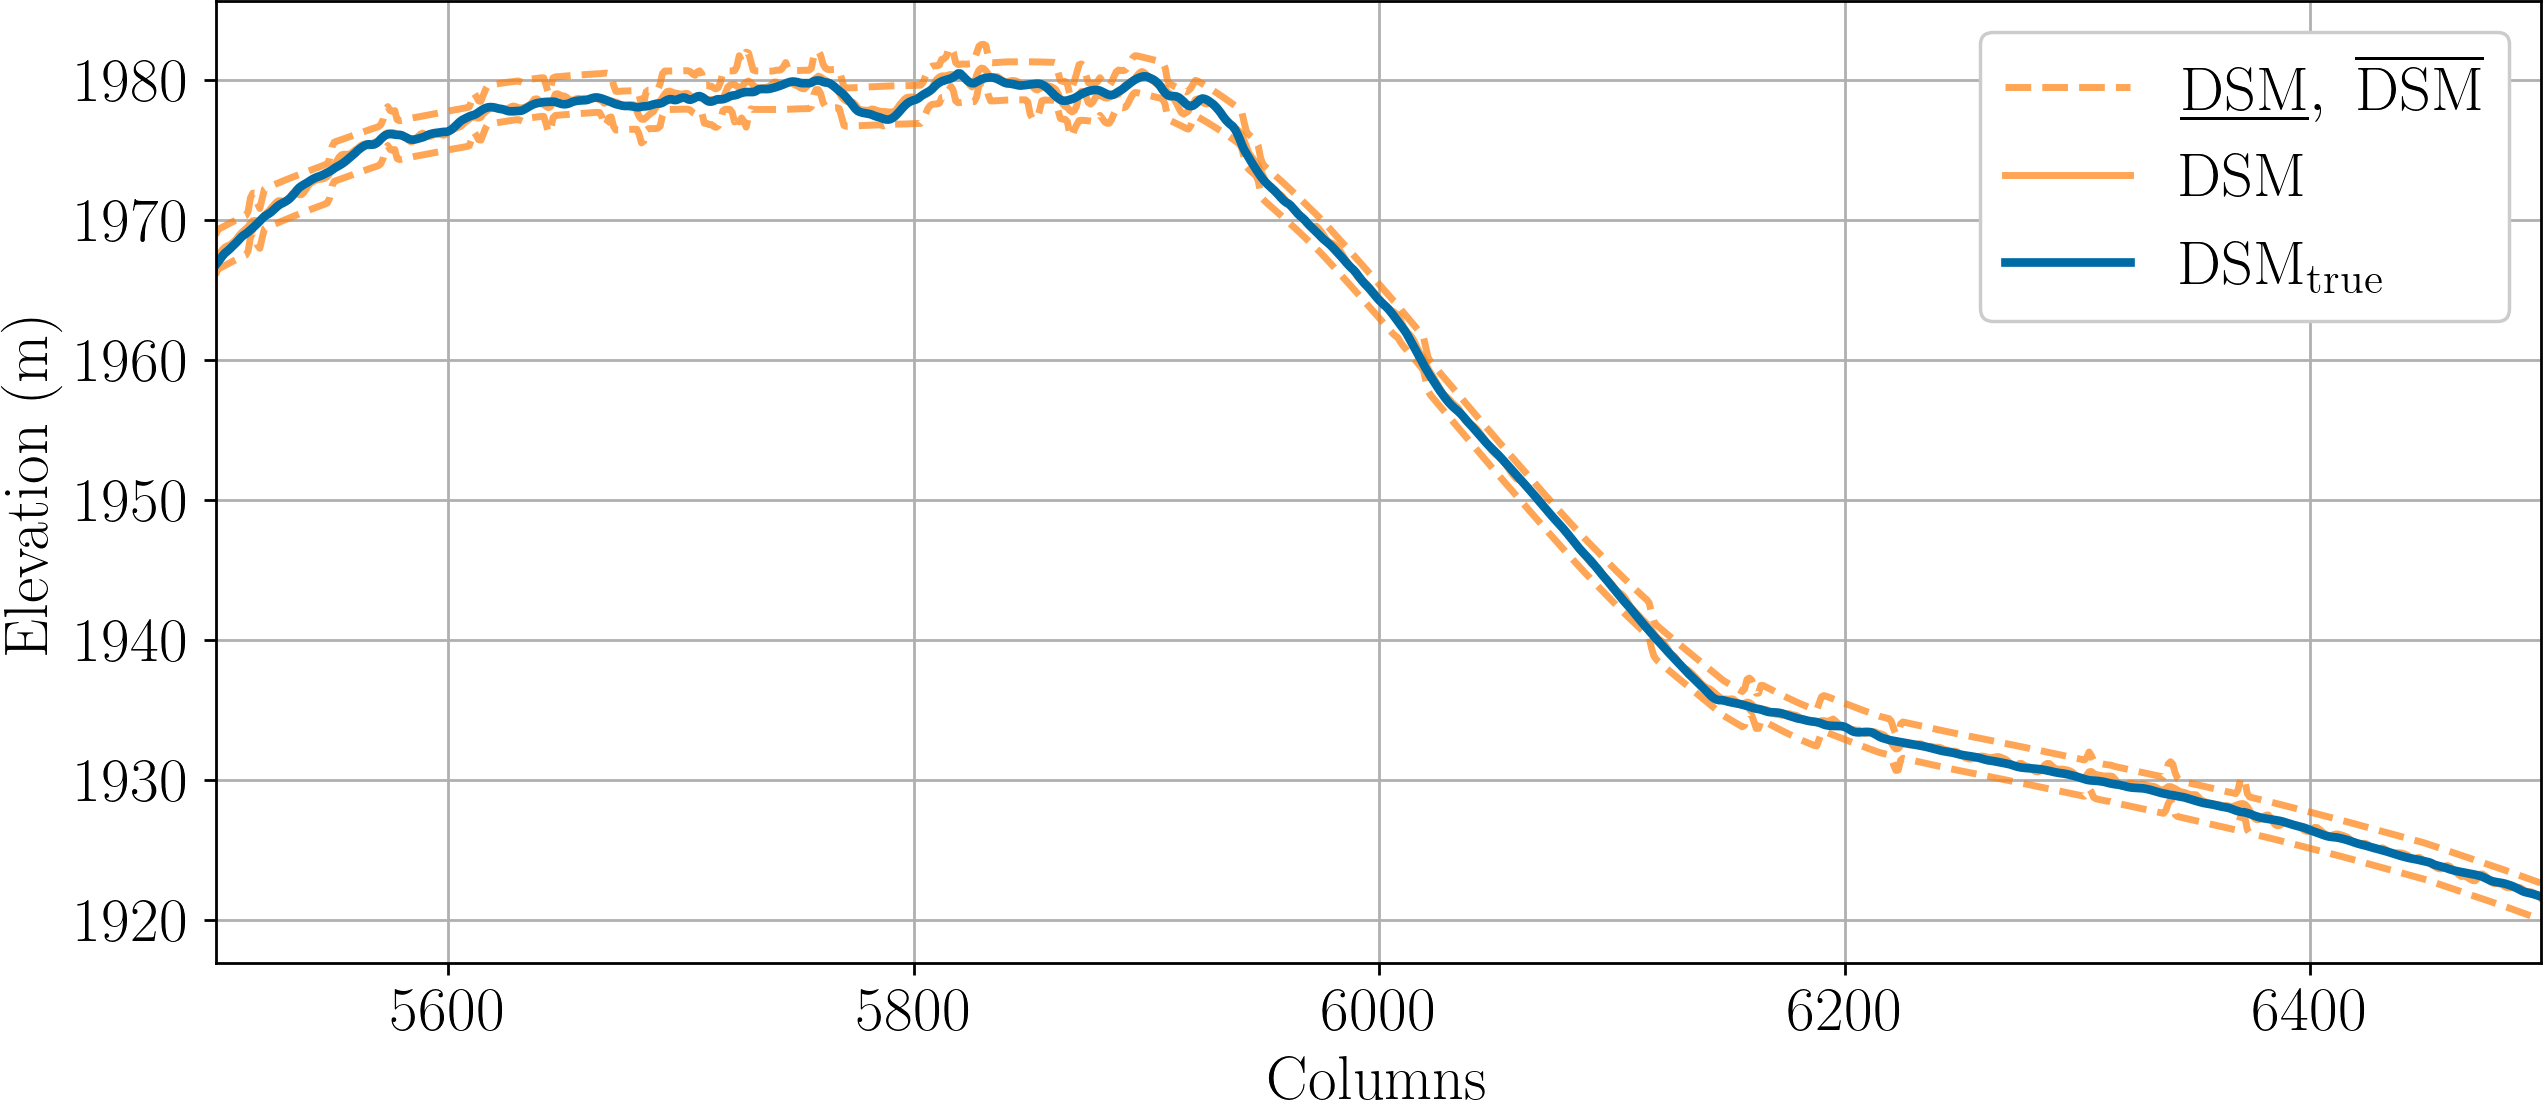
\includegraphics[width=\linewidth]{Images/Chap_6/Graasubreen_row_1500.png}
        \caption{\acrshort{dsm}, ground truth and elevation intervals along the orange line of \subref{fig:Graasubreen_dsm_zoom}}
        \label{fig:Graasubreen_zoom_row}
    \end{subfigure}
    \caption{Details of the Graasubreen \acrshort{dsm}. This area corresponds to the orange square from \Cref{fig:Graasubreen_dsm}.}
    \label{fig:Graasubreen_zoom}
\end{figure}


\begin{figure}
    \begin{subfigure}[t]{0.549\linewidth}
        \flushleft
        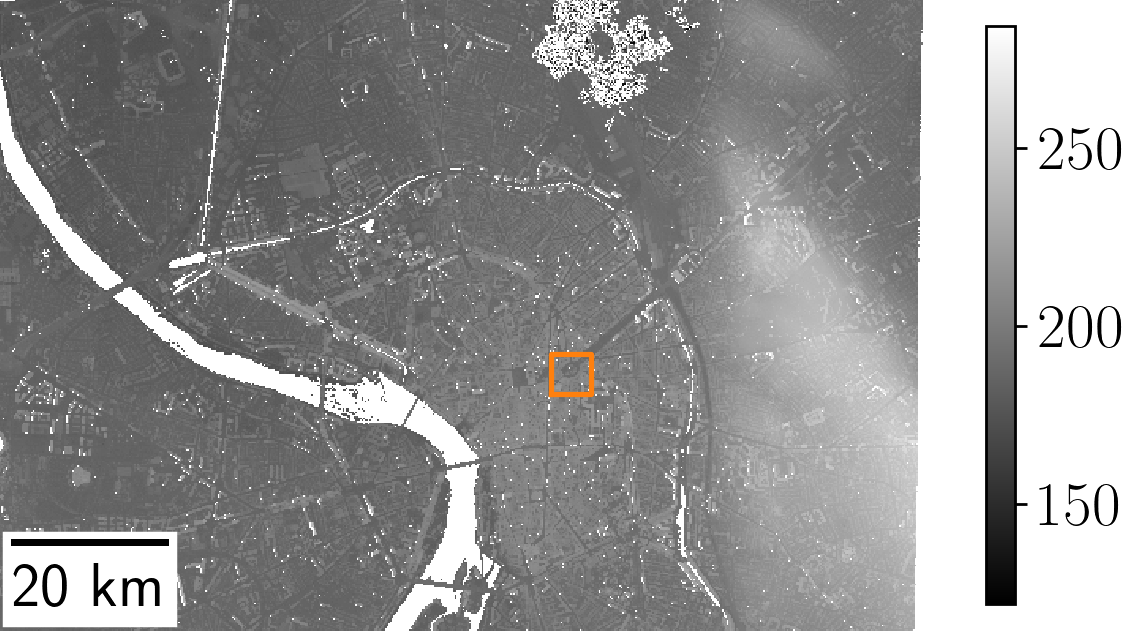
\includegraphics[width=\linewidth]{Images/Chap_6/Toulouse_dsm.png}
        \caption{Photogrammetry \acrshort{dsm}. Orange area is detailed in \Cref{fig:toulouse_zoom}}
        \label{fig:toulouse_dsm}
    \end{subfigure}
    \begin{subfigure}[t]{0.451\linewidth}
        \flushright
        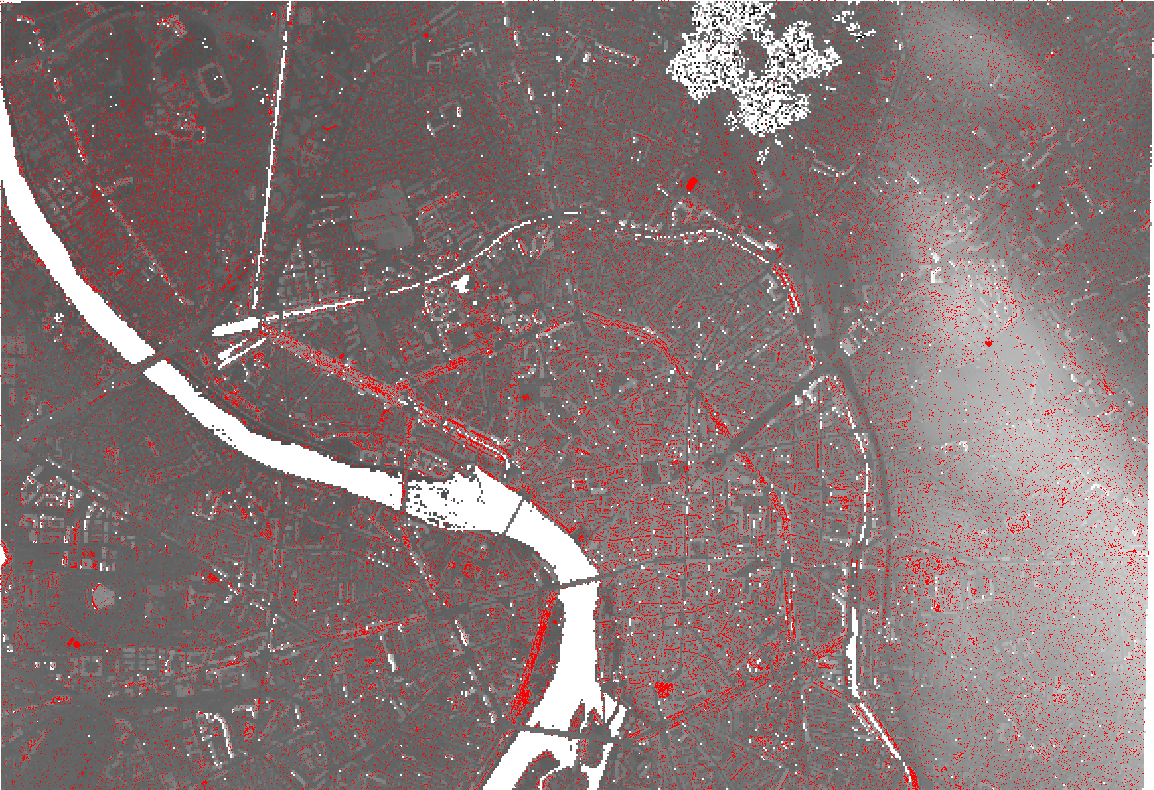
\includegraphics[width=\linewidth]{Images/Chap_6/Toulouse_error.png}
        \caption{\acrshort{dsm} with wrong intervals in red.}
        \label{fig:toulouse_error}
    \end{subfigure}
    \caption{\acrshort{dsm} without and with wrong intervals over Toulouse scene}
    \label{fig:toulouse_global}
\end{figure}

\begin{figure}
    \begin{subfigure}[t]{0.49\linewidth}
        \flushleft
        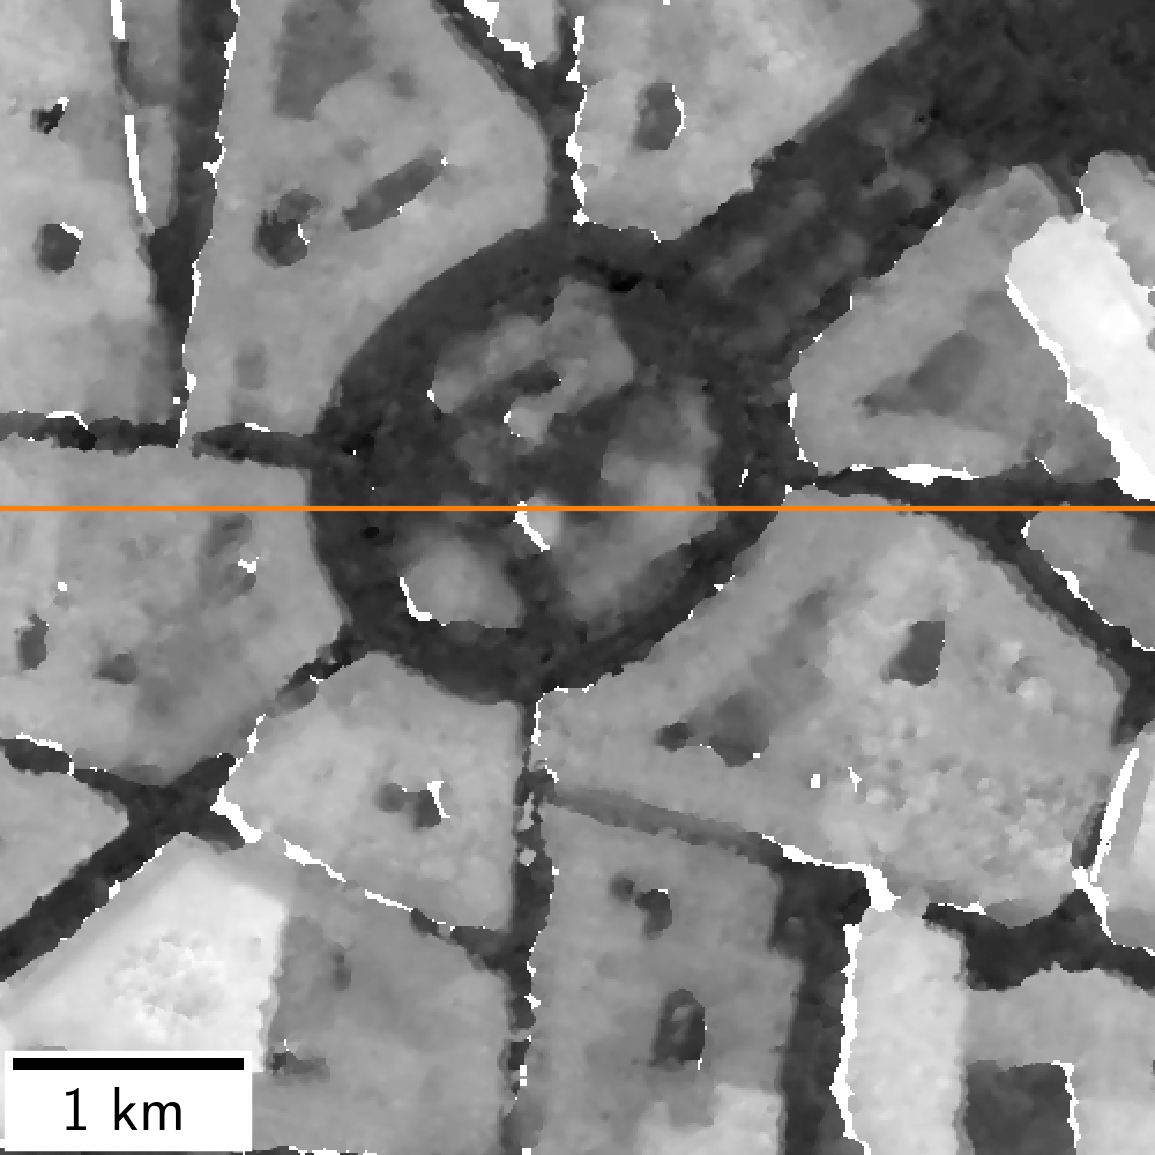
\includegraphics[width=\linewidth]{Images/Chap_6/Toulouse_dsm_zoom.png}
        \caption{Photogrammetry \acrshort{dsm}. Orange line is detailed in \Cref{fig:toulouse_zoom_row}}
        \label{fig:toulouse_dsm_zoom}
    \end{subfigure}\hfill
    \begin{subfigure}[t]{0.49\linewidth}
        \flushright
        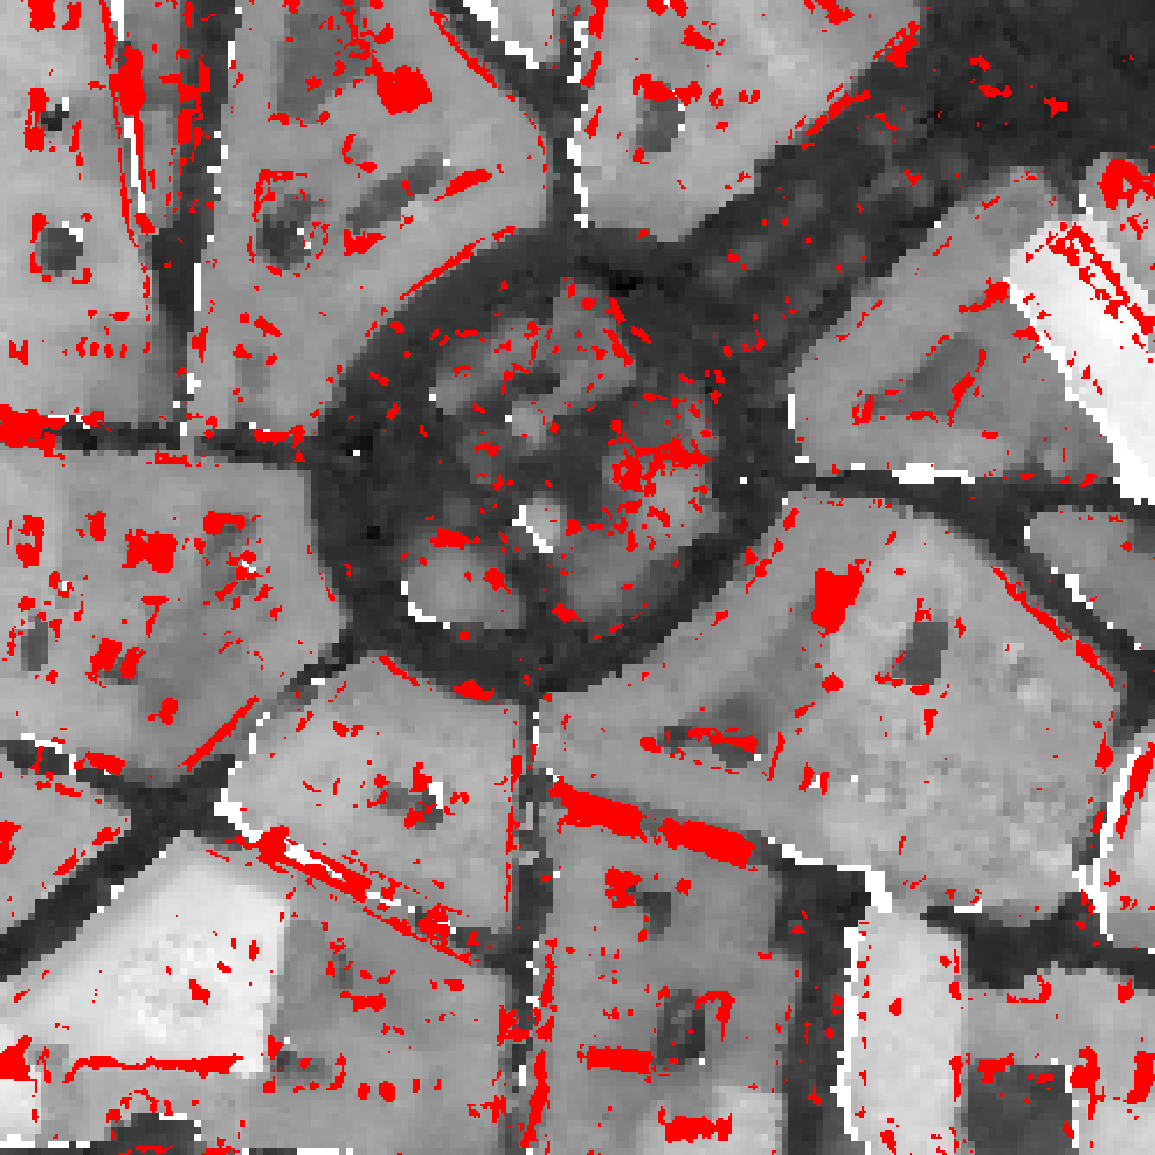
\includegraphics[width=\linewidth]{Images/Chap_6/Toulouse_error_zoom.png}
        \caption{\acrshort{dsm} with wrong intervals in red.}
        \label{fig:toulouse_error_zoom}
    \end{subfigure}
    \begin{subfigure}[t]{\linewidth}
        \centering
        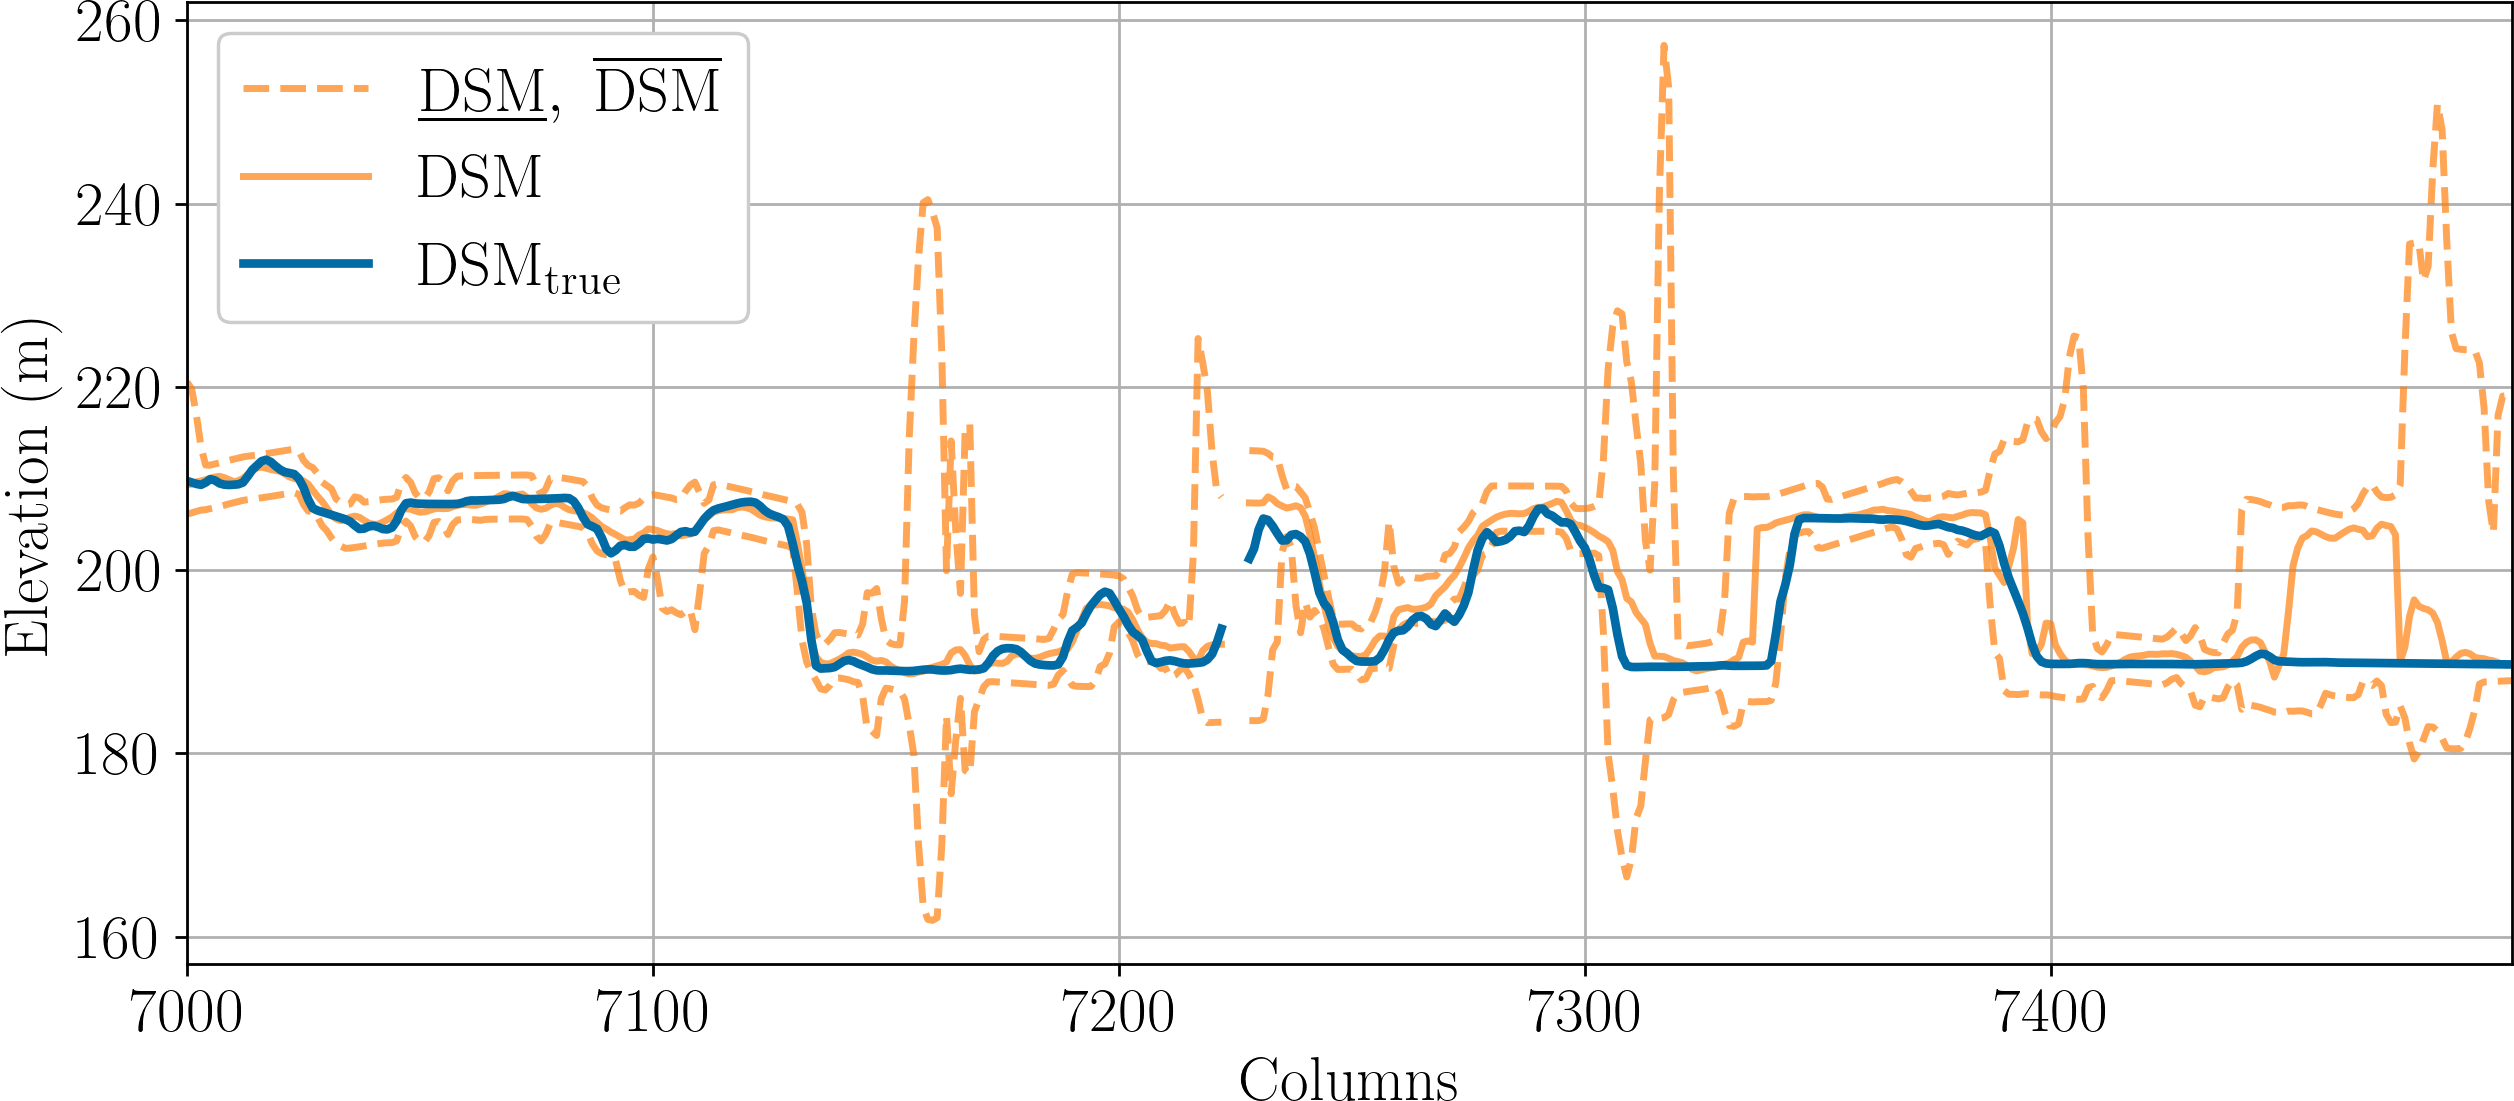
\includegraphics[width=\linewidth]{Images/Chap_6/Toulouse_row_4720.png}
        \caption{\acrshort{dsm}, ground truth and elevation intervals along the orange line of \Cref{fig:toulouse_dsm_zoom}}
        \label{fig:toulouse_zoom_row}
    \end{subfigure}
    \caption{Detailed \acrshort{dsm} over Wilson square, Toulouse. This area corresponds to the orange square from \Cref{fig:toulouse_dsm}.}
    \label{fig:toulouse_zoom}
\end{figure}

\begin{figure}
    \begin{subfigure}[t]{0.3\linewidth}
        \flushleft
        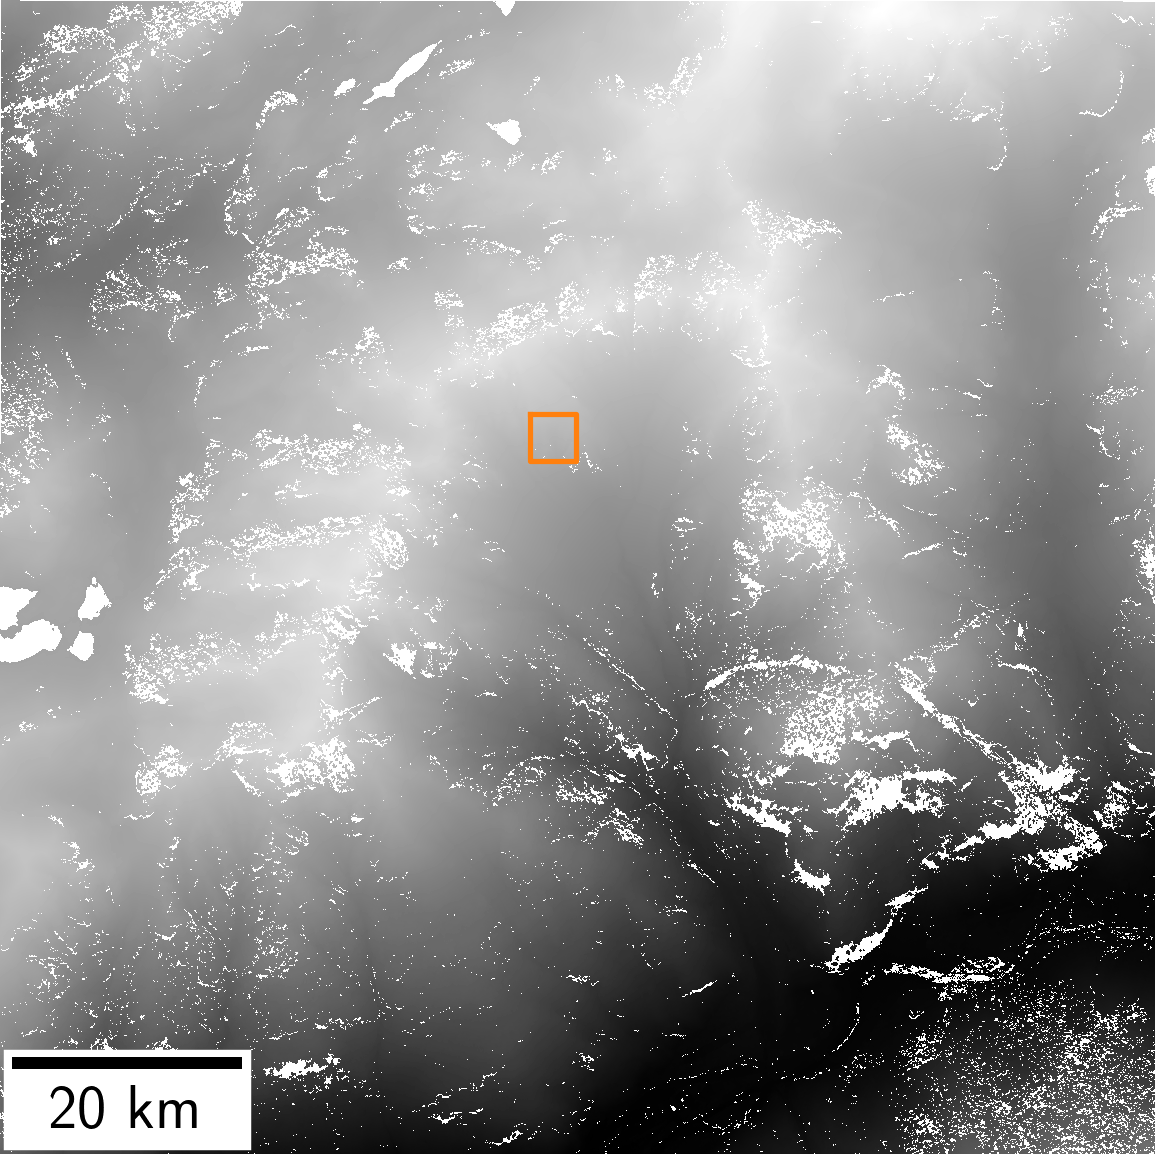
\includegraphics[width=\linewidth]{Images/Chap_6/Grenoble_dsm_full_3600-4000_4600-5000.png}
        \caption{Photogrammetry \acrshort{dsm}. Orange square is detailed in \subref{fig:grenoble_dsm_full}}
        \label{fig:grenoble_dsm_full}
    \end{subfigure}\hfill
    \begin{subfigure}[t]{0.3\linewidth}
        \centering
        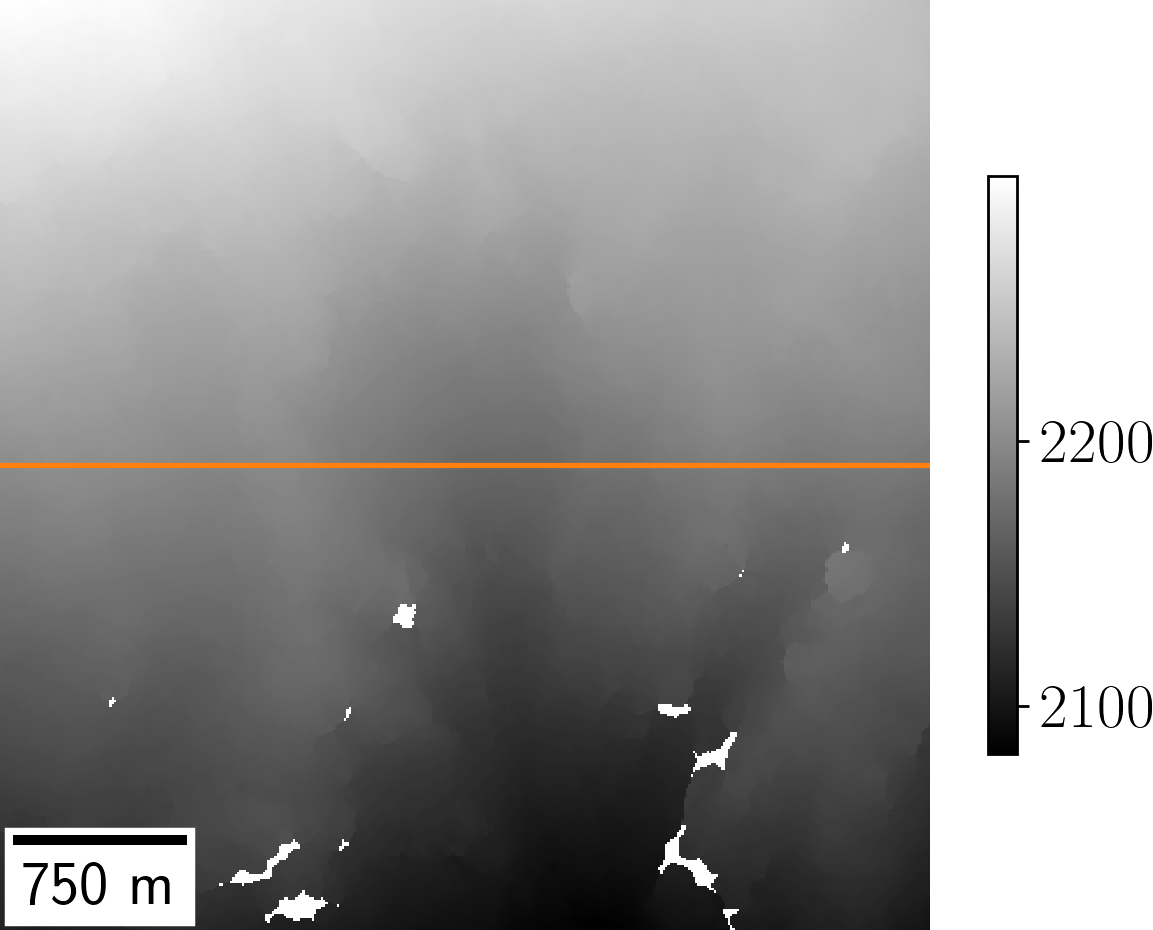
\includegraphics[width=\linewidth]{Images/Chap_6/Grenoble_dsm_zoom_3600-4000_4600-5000.png}
        \caption{Photogrammetry \acrshort{dsm} zoom. Orange line is detailed in \subref{fig:grenoble_zoom_row}}
        \label{fig:grenoble_dsm_zoom}
    \end{subfigure}\hfill
    \begin{subfigure}[t]{0.3\linewidth}
        \flushright % k=h1/h2*w2/w1
        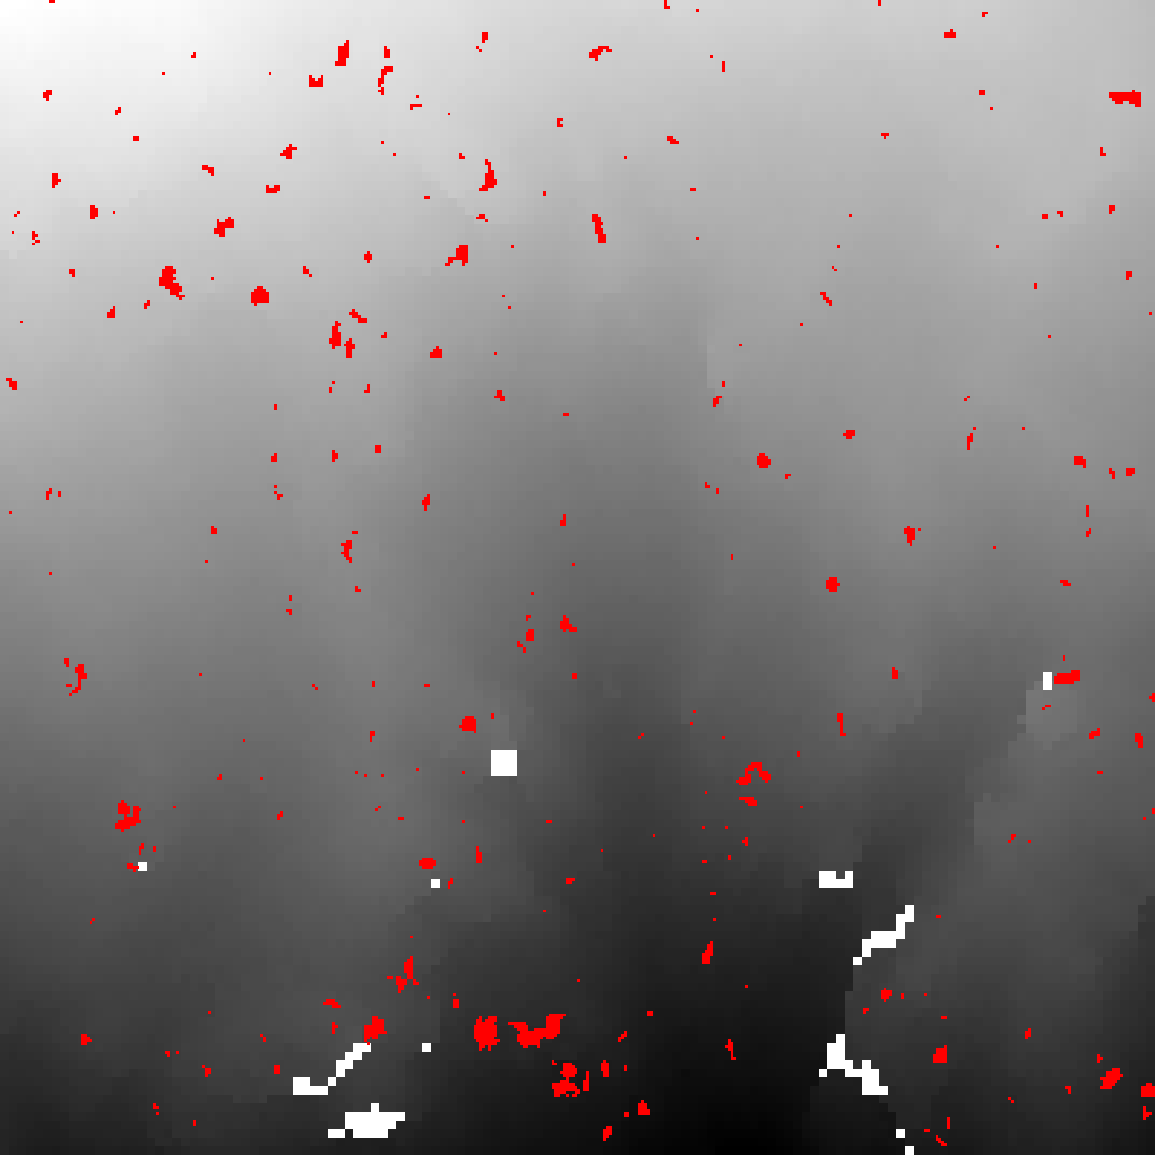
\includegraphics[width=0.807\linewidth]{Images/Chap_6/Grenoble_error_zoom_3600-4000_4600-5000.png}
        \caption{\acrshort{dsm} with wrong intervals in red.}
        \label{fig:grenoble_error_zoom}
    \end{subfigure}\\
    \begin{subfigure}[t]{\linewidth}
        \centering
        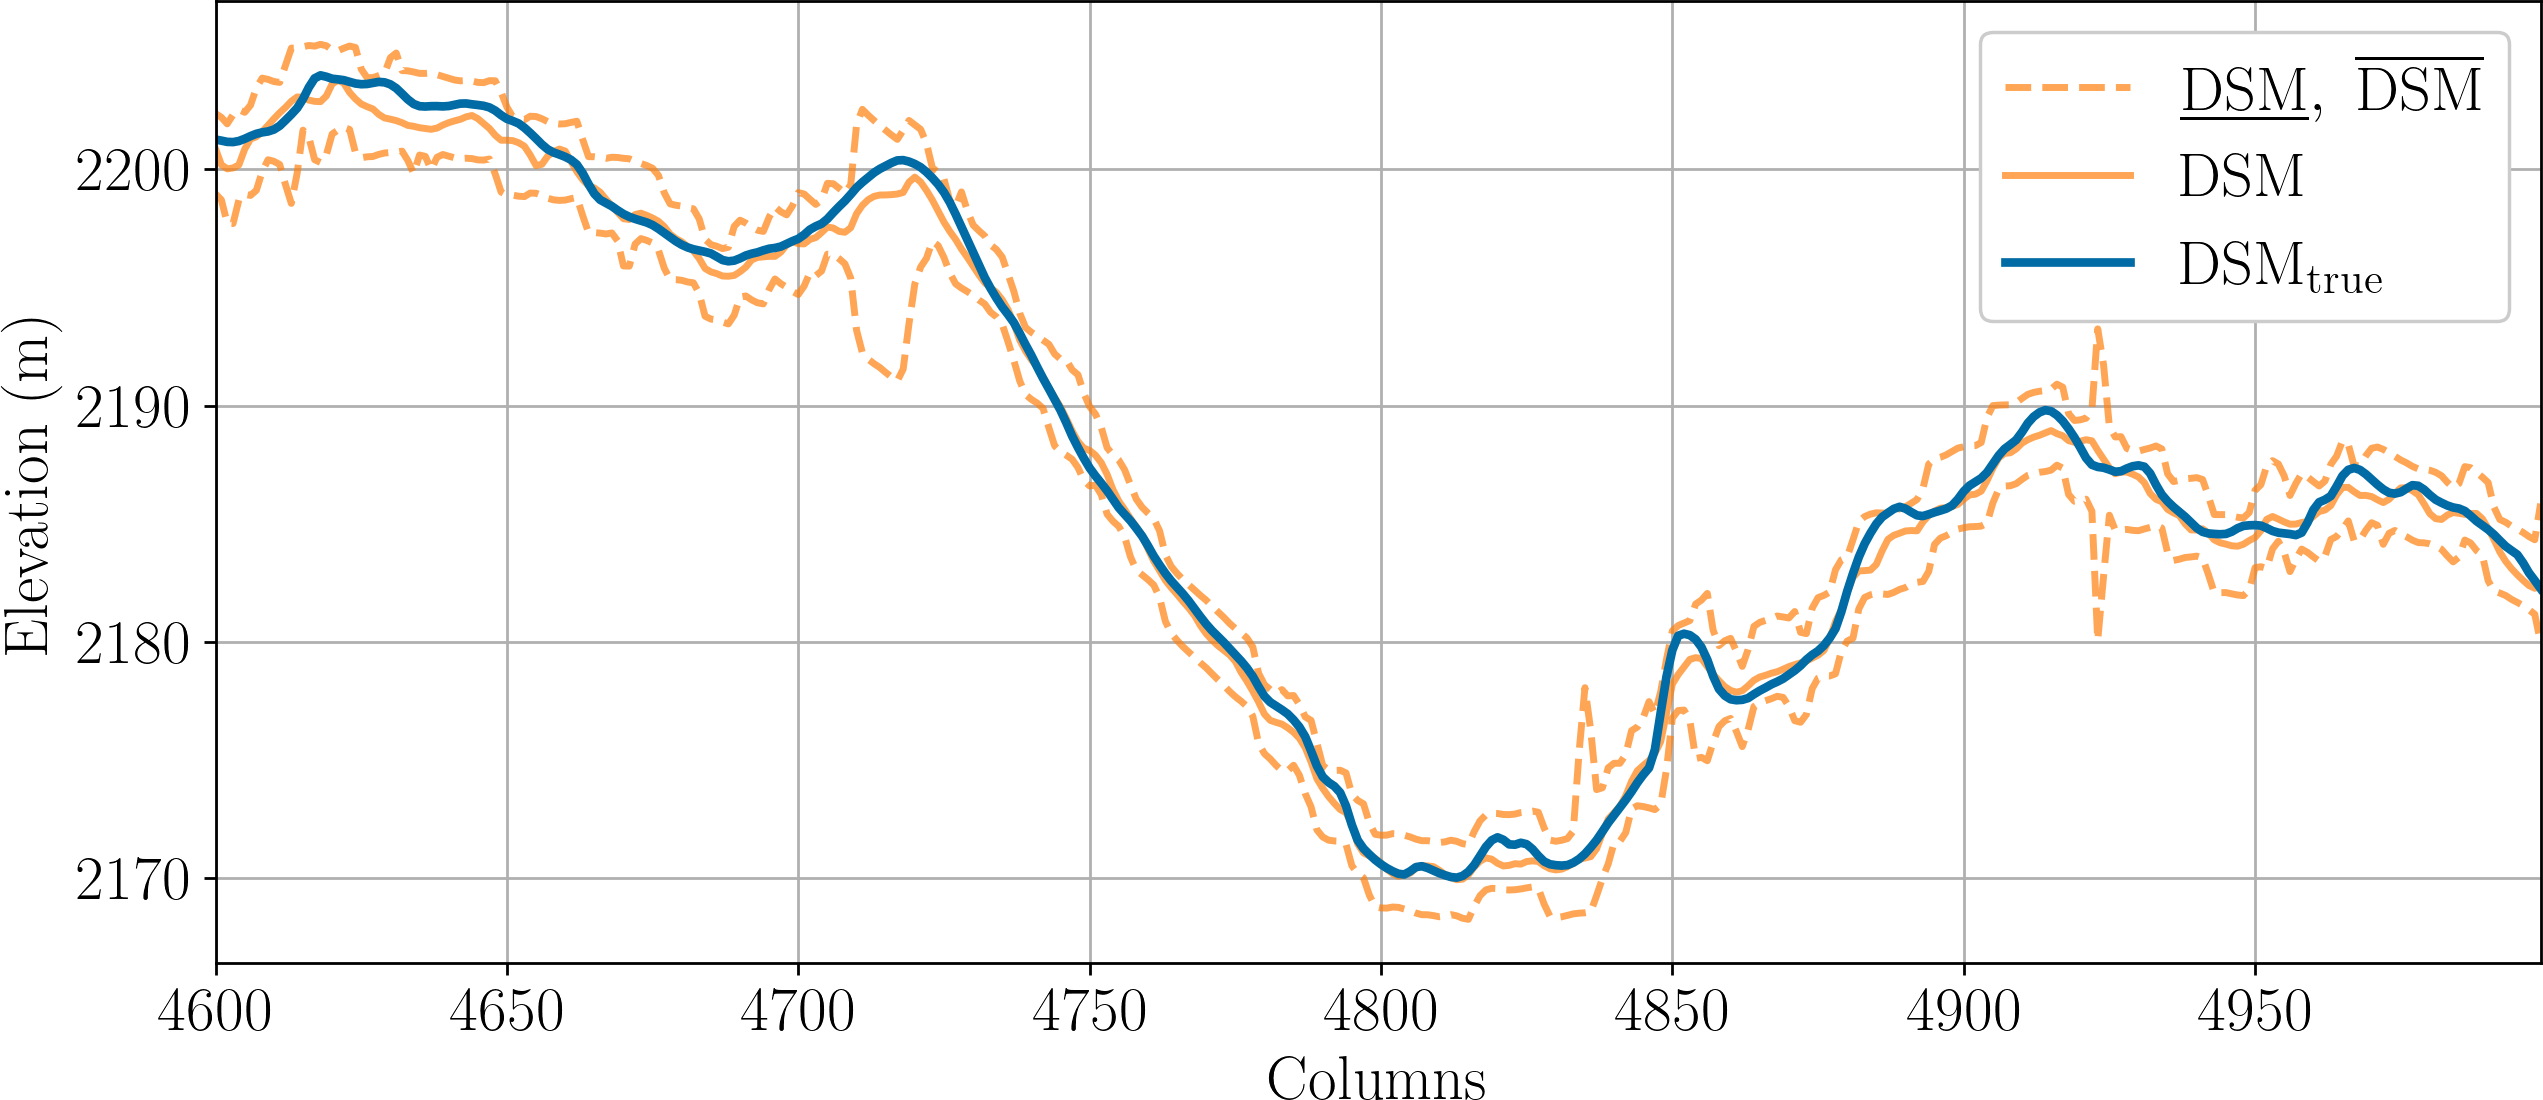
\includegraphics[width=\linewidth]{Images/Chap_6/Grenoble_row_3800.png}
        \caption{\acrshort{dsm}, ground truth and elevation intervals along the orange line of \Cref{fig:grenoble_dsm_zoom}}
        \label{fig:grenoble_zoom_row}
    \end{subfigure}
    \caption{Detailed \acrshort{dsm} over the mountainous region near Grenoble.}
    \label{fig:grenoble_zoom}
\end{figure}

\begin{figure}
    \begin{subfigure}[t]{0.3\linewidth}
        \flushleft
        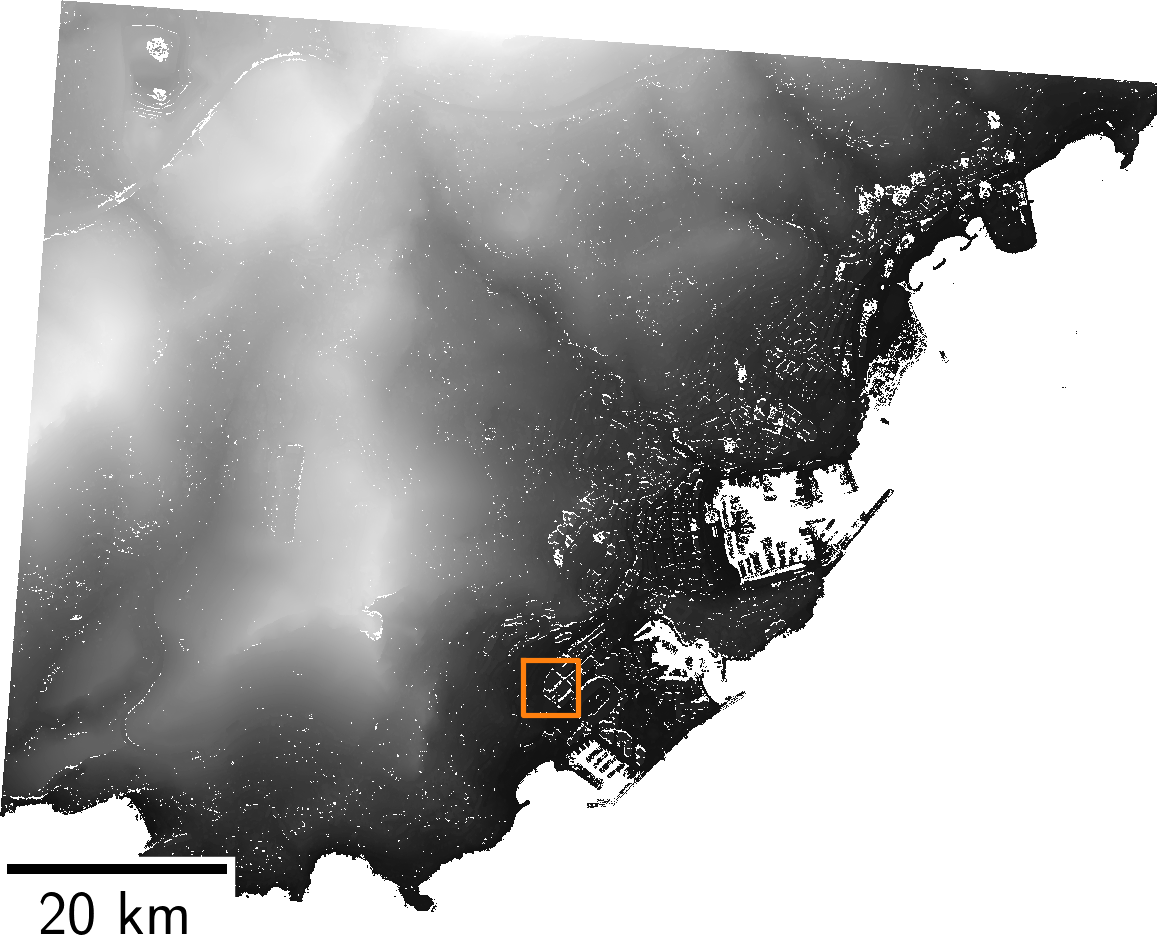
\includegraphics[width=\linewidth]{Images/Chap_6/Monaco_dsm_full_6000-6500_4800-5300.png}
        \caption{Photogrammetry \acrshort{dsm}. Orange square is detailed in \subref{fig:monaco_dsm_full}}
        \label{fig:monaco_dsm_full}
    \end{subfigure}\hfill
    \begin{subfigure}[t]{0.3\linewidth}
        \centering
        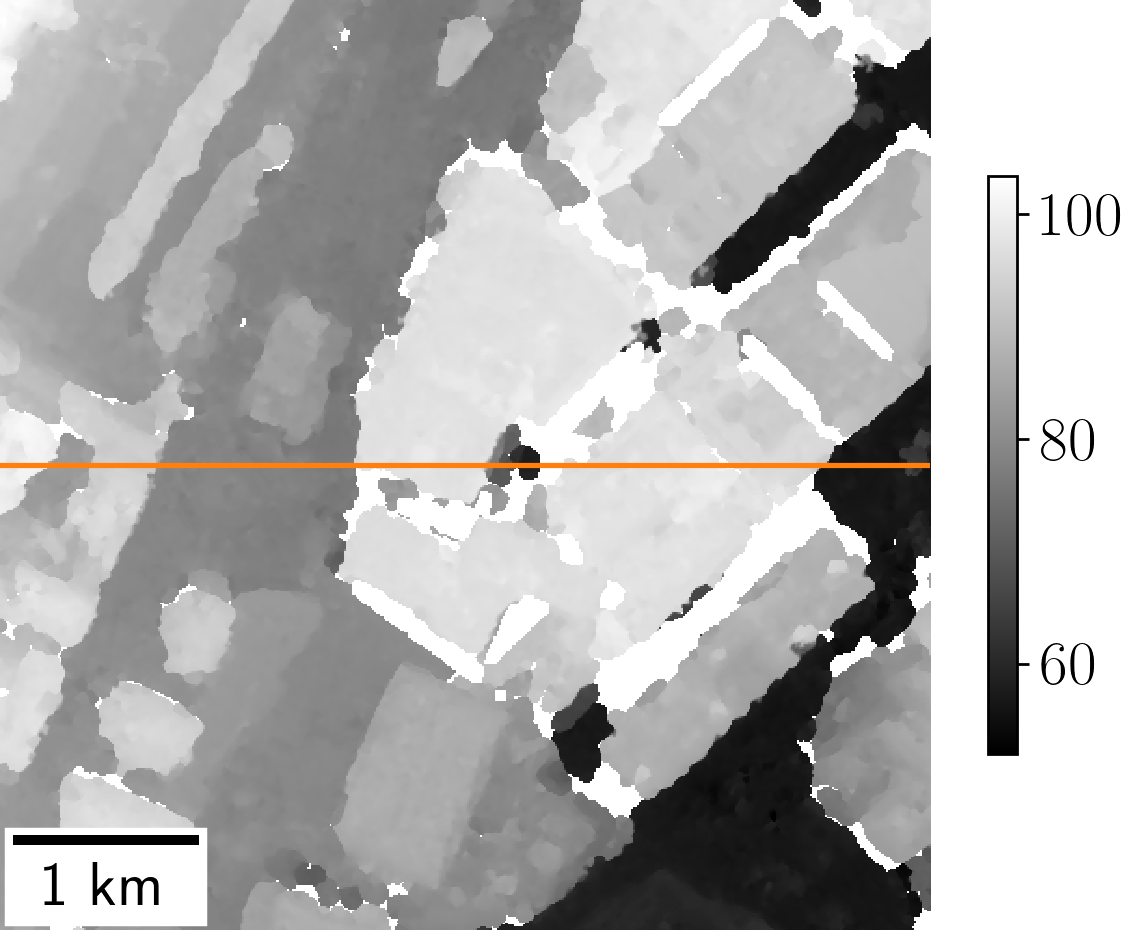
\includegraphics[width=\linewidth]{Images/Chap_6/Monaco_dsm_zoom_6000-6500_4800-5300.png}
        \caption{Photogrammetry \acrshort{dsm} zoom. Orange line is detailed in \subref{fig:monaco_zoom_row}}
        \label{fig:monaco_dsm_zoom}
    \end{subfigure}\hfill
    \begin{subfigure}[t]{0.3\linewidth}
        \flushright
        \includegraphics[width=0.83\linewidth]{Images/Chap_6/Monaco_error_zoom_6000-6500_4800-5300.png}
        \caption{\acrshort{dsm} with wrong intervals in red.}
        \label{fig:monaco_error_zoom}
    \end{subfigure}\\
    \begin{subfigure}[t]{\linewidth}
        \centering
        \includegraphics[width=\linewidth]{Images/Chap_6/Monaco_row_6250.png}
        \caption{\acrshort{dsm}, ground truth and elevation intervals along the orange line of \subref{fig:monaco_dsm_zoom}}
        \label{fig:monaco_zoom_row}
    \end{subfigure}
    \caption{Detailed \acrshort{dsm} over the city of Monaco.}
    \label{fig:monaco_zoom}
\end{figure}

\begin{figure}
    \begin{subfigure}[t]{0.3\linewidth}
        \flushleft
        \includegraphics[width=\linewidth]{Images/Chap_6/Langfjordjokelen_dsm_full_1850-2250_2250-2750.png}
        \caption{Photogrammetry \acrshort{dsm}. Orange square is detailed in \subref{fig:langfjordjokelen_dsm_zoom}}
        \label{fig:langfjordjokelen_dsm_full}
    \end{subfigure}\hfill
    \begin{subfigure}[t]{0.3\linewidth}
        \centering
        \includegraphics[width=\linewidth]{Images/Chap_6/Langfjordjokelen_dsm_zoom_1850-2250_2250-2750.png}
        \caption{Photogrammetry \acrshort{dsm} zoom. Orange line is detailed in \subref{fig:langfjordjokelen_zoom_row}}
        \label{fig:langfjordjokelen_dsm_zoom}
    \end{subfigure}\hfill
    \begin{subfigure}[t]{0.3\linewidth}
        \flushright
        \includegraphics[width=0.809\linewidth]{Images/Chap_6/Langfjordjokelen_error_zoom_1850-2250_2250-2750.png}
        \caption{\acrshort{dsm} with wrong intervals in red.}
        \label{fig:langfjordjokelen_error_zoom}
    \end{subfigure}\\
    \begin{subfigure}[t]{\linewidth}
        \centering
        \includegraphics[width=\linewidth]{Images/Chap_6/Langfjordjokelen_row_2000.png}
        \caption{\acrshort{dsm}, ground truth and elevation intervals along the orange line of \subref{fig:langfjordjokelen_dsm_zoom}}
        \label{fig:langfjordjokelen_zoom_row}
    \end{subfigure}
    \caption{Detailed \acrshort{dsm} over the Langfjordjøkelen glacier.}
    \label{fig:langfjordjokelen_zoom}
\end{figure}

The different metrics have been evaluated between the photogrammetry \acrshort{dsm} and the associated ground truth \acrshort{dsm}. Results are presented in \Cref{tab:elevation_metrics_global}, and are commented in the following sections. We also displayed for informational purposes the proportion of invalid pixels of each scene, in the last column of the table. A pixel is invalid if the ground truth \acrshort{dsm} or predicted \acrshort{dsm} does not contain any data for this pixel, or if it was masked by a water mask. Invalid pixels are therefore pixels that were not considered when computing the metrics.

\Cref{fig:Graasubreen_global,fig:Graasubreen_zoom,fig:toulouse_global,fig:toulouse_zoom,fig:grenoble_zoom,fig:monaco_zoom,fig:langfjordjokelen_zoom} allow to qualitatively evaluate the performance of the elevation intervals in different scenes. We can see that intervals seem to have a better accuracy performance in rural scenes such as glaciers than in urban scenes. For instance, we can clearly see wrong intervals of the Toulouse scene in \Cref{fig:toulouse_error}. They are harder to distinguish in the Graasubreen scene in \Cref{fig:Graasubreen_error,fig:Graasubreen_error_zoom}. Another notable observation is that elevation intervals of the Graasubreen glacier in \Cref{fig:Graasubreen_zoom_row} are very small and do not present large size fluctuations along the considered cross-section. This is not the case for the Toulouse scene (\Cref{fig:toulouse_zoom_row}), where intervals present large variations in size. They are relatively small from columns 7000 to 7100, but their size increase from column 7400 to 7500. We can see on the right of \Cref{fig:toulouse_zoom_row}, near column 7450, that their size allow to correctly contain the ground truth despite the difference between $\DSM$ and $\DSM_{true}$. However, there are some very large intervals, sometimes reaching $80$ m in size, near columns 7150, or 7300. Those intervals can occur because the range of considered disparities in the dense matching step is $[-50, 50]$, for every scene. Converted into altitude, elevations intervals have a maximal size of $[-50\cdot r_{alt}, 50\cdot r_{alt}]$, centered around the reference altitude (which can vary across the scene). This means that we can have a maximal elevation interval of size 243m in the case of Toulouse, where $r_{alt}=2.43$. The previously observed intervals of size 80m in \Cref{fig:toulouse_zoom_row} thus originates from a disparity interval of 33 pixels in size, \ie a third of the disparity intervals. Other examples of large intervals include the Monaco scene where $r_{alt}=0.99$ and for which the largest interval has a size of $99$ m, or the Paris scene where  $r_{alt}=5.78$ and the largest interval has a size of 578m. We will see in section \ref{sec:unexplored_leads} that we can modify our method to filter out points leading to those intervals. For now, we will evaluate the method as it stands. The following sections are dedicated to discussing each metric individually.

\subsection{Elevation Accuracy}
The elevation accuracy $Z_{acc}$, defined in \Cref{eq:relative_accuracy_elevation}, measures the proportions of intervals which contains the ground truth elevation, which we want to be as high as possible. The first observation is that the $90\%$ accuracy objective is validated on $8$ of the $11$ scenes we considered. In particular, the different glaciers as well as the Pic du Midi elevation intervals present a great accuracy, between $98.1\%$ and $99.7\%$. Scenes that do not verify the $90\%$ objective are the urban stereo pairs over Bordeaux, Montpellier, and Paris. In general, it seems that urban \acrshort{dsm}s have a lower accuracy than rural ones, which was to be expected as there are more steep variations of elevation in cities due to the presence of buildings. The Montpellier \acrshort{dsm} and Bordeaux \acrshort{dsm} are close to the $90\%$ objective, but intervals over Paris present an elevation accuracy of only $84.6\%$ . We will see in \Cref{sec:other_errors} that some other sources of errors can explain why $Z_{acc}<90\%$ on those scenes, such as vibration of the satellite during images acquisition or ground truth non-synchronicity issues. Provided that those errors are not present, we can claim that elevation intervals are accurate enough. They correctly estimate the error committed during the dense matching step, and the propagation of disparity intervals to elevation intervals is properly carried out.

\subsection{Residual Elevation Error}
The residual elevation error $Z_\varepsilon$, defined in \Cref{eq:residual_error_elevation}, estimates the gap between intervals and the ground truth, when intervals do not contain the ground truth. We want it to be as small as possible. $Z_\varepsilon$ is less than, or almost equal to, half a pixel for the majority of scenes, which is also around $0.5\%$ of the disparity range. This is really low, especially when compared to disparity intervals of \Cref{tab:metric_average} where $\varepsilon$ was typically around $3\%$ of the disparity range. Because $Z_\varepsilon$ is the median of error, it means that half of wrong intervals are less than $Z_\varepsilon$ pixels away from one of the bounds of the elevation intervals. Consequently, extending intervals by $Z_\varepsilon$ would divide by two the number of wrong intervals. For instance, on the Monaco scene, $Z_\varepsilon=0.57$pix, $r_{alt}=0.99$ m/pix and $Z_{acc}=90.3\%$. Defining the extended intervals as:
\begin{align*}
    [\underline{\DSM}-Z_\varepsilon\cdot r_{alt}, \overline{\DSM}+Z_\varepsilon\cdot r_{alt}] \approx [\underline{\DSM}-0.56, \overline{\DSM}+0.56]
\end{align*}
As the accuracy is $90.3\%$, it means that $9.7\%$ of pixels are not accurate. Using $[\underline{\DSM}-0.56, \overline{\DSM}+0.56]$ would lead to a new accuracy of $90.3+\dfrac{9.7}{2}=95.15\%$. For every scene, validating the $90\%$ accuracy, $Z_\varepsilon$ provides an easy extension for obtaining intervals with $95\%$ accuracy.

\Cref{fig:histogram_elevation_error} displays histograms of the distribution of errors, from which $Z_\varepsilon$ is the median. For both urban and rural scenes, errors are mostly of a few pixels. The shape of distributions on other scenes are similar to the Toulouse or Pic du Midi scenes. There is one $Z_\varepsilon$ value that stands out, for the Hellmem scene, where it equals $2.76$ pixels. \Cref{fig:error_hist_hellmem} displays the distribution of errors on the Hellmem scene, where the majority of the distribution is still located on the first peak of the distribution. There is however the presence of a tail on the distributions, that was not present on other scenes. We have to keep in mind that the accuracy for this scene is $98.8\%$, so that $Z_\varepsilon$ is only computed on $1.2\%$ of valid intervals. $Z_\varepsilon=2.76$ is therefore not necessarily a concerning observation, as it concerns very few pixels. It is more surprising that it equals $0.12$ for the Graasubreen \acrshort{dsm} which already has the best accuracy ($99.7\%$) out of all scenes. This translates the great accuracy performance of the elevation intervals estimation on this area.

\begin{figure}
    \centering
    \begin{subfigure}[t]{0.49\linewidth}
        \flushleft
        \includegraphics[width=\linewidth]{Images/Chap_6/histogram_elevation_eps_Toulouse.png}
        \caption{Toulouse}
        \label{fig:error_hist}
    \end{subfigure}\hfill
    \begin{subfigure}[t]{0.49\linewidth}
        \flushright
        \includegraphics[width=\linewidth]{Images/Chap_6/histogram_elevation_eps_Pic_du_midi.png}
        \caption{Pic du Midi}
        \label{fig:error_hist_pic_du_midi}
    \end{subfigure}\vspace*{0.3cm}\\
    \centering
    \begin{subfigure}[t]{0.49\linewidth}
    \centering
        \includegraphics[width=\linewidth]{Images/Chap_6/histogram_elevation_eps_Hellmem.png}
        \caption{Hellmem}
        \label{fig:error_hist_hellmem}
    \end{subfigure}
    \caption{Histograms of the residual error over the Toulouse, Pic du Midi and Hellmem scenes. $Z_{\varepsilon}$ is defined as the median of those distributions.}
    \label{fig:histogram_elevation_error}
\end{figure}

\subsection{Relative Elevation Size}
The relative elevation size $Z_{size}$, defined in \Cref{eq:relative_size_elevation}, estimates the size of intervals, both correct and incorrect. $Z_{size}$ is usually around 2 pixels wide. The Bordeaux, Grenoble and Monaco datasets are the only exceptions, where $Z_{size}$ is closer to 4 pixels in size. It does not seem to be correlated neither to the accuracy, nor to the altimetric ratio or acquisition angles of the satellites. In any case, 4 pixels is not ideal, but it is not excessively large either, especially as the considered disparity range is $[-50,50]$ in pixels. We can deduce from those values of $Z_{size}$ that the predicted \acrshort{dsm} is close to the true elevation. 

\Cref{fig:histogram_elevation_size} presents the distributions of relative sizes over the Toulouse and Hellmem scenes. It provides a more complete overview of the distribution of sizes than simply the indicator $Z_{size}$ which is defined as the median of those distributions. The distributions on other scenes have a similar shape.

\begin{figure}
    \centering
    \begin{subfigure}[t]{0.49\linewidth}
        \flushleft
        \includegraphics[width=\linewidth]{Images/Chap_6/histogram_elevation_s_rel_Toulouse.png}
        \caption{Toulouse}
        \label{fig:size_hist}
    \end{subfigure}\hfill
    \begin{subfigure}[t]{0.49\linewidth}
        \flushright
        \includegraphics[width=\linewidth]{Images/Chap_6/histogram_elevation_s_rel_Pic_du_midi.png}
        \caption{Pic Du Midi}
        \label{fig:size_hist_pic_du_midi}
    \end{subfigure}
    \caption{Histograms of the relative size over the Toulouse and Pic du Midi scenes. $Z_{size}$ is defined as the median of those distributions.}
    \label{fig:histogram_elevation_size}
\end{figure}

\subsection{Altimetric Ratio and Invalid Pixels}
Looking at \Cref{tab:elevation_metrics_global}, it seems that high values of the altimetric ratio $r_{alt}$ are correlated to ``low'' values of accuracy. This correlation does not imply a causal relationship. Indeed, scenes with low accuracy are urban scenes, on which the 3D reconstruction is harder due to the strong variations of elevation. In order to limit the number of occlusions in urban scenes, we often reduce the convergence angle of satellites. A low convergence angle results in a high altimetric ratio, as seen in \Cref{fig:incidence_angle}. This explains why we observe a high altimetric ratio for scenes with low accuracy.

The proportion of invalid pixels that are not considered in the metrics can sometimes be quite high, as it is the case for Monaco (41$\%$) or Hellmem (34.7$\%$). This is due to the presence of water in large part of the image (\Cref{fig:miniature_Monaco_rgb}) or simply the absence of data from the provided ground truth (\Cref{fig:miniature_Hellmem_gt})

\section{Comparison with ``Naive'' Intervals}
The fact that most intervals have a relative size $Z_{size}$ of around 2 pixels may raise the following question: would ``naive'' intervals be accurate ? We define naive intervals $[\underline{\DSM}_{naive}, ~\overline{\DSM}_{naive}]$, as intervals centered on the predicted \acrshort{dsm} with a size of 2 times the altimetric ratio $r_{alt}$:
\begin{align}
    [\underline{\DSM}_{naive}, ~\overline{\DSM}_{naive}] = [\DSM-r_{alt}, \DSM+r_{alt}]
\end{align}
\Cref{tab:naive_accuracy} allows comparing the accuracy of the naive intervals with that of our interval method. The table also contains the mean and median errors of the \acrshort{dsm} defined as:
\begin{align}
    \varepsilon_{\mean} = \mean|\DSM - \DSM_{true}|\qquad \varepsilon_{\median} = \median|\DSM - \DSM_{true}|
\end{align}

\begin{table}[ht]
    \centering
    \begin{tabular}{|c||c|c|c|c|}
        \hline
        Scene & $Z_{acc}$ (pix) & ``Naive'' $Z_{acc}$ (pix) & $\varepsilon_{\median}$ (m) & $\varepsilon_{\mean}$ (m)
        \\\hline\hline
        Bordeaux & 89.3$\%$ & 62.9$\%$ & 0.86 & 1.93\\\hline
        Graasubreen & 99.7$\%$ & 98.8$\%$ & 0.19 & 0.28\\\hline
        Hellmem & 98.8$\%$ & 96.4$\%$ & 0.22 & 0.75\\\hline
        Grenoble & 93.1$\%$ & 65.7$\%$ & 0.61 & 2.08\\\hline
        Langfjordjøkelen & 99.4$\%$ & 88.1$\%$ & 0.26 & 1.31\\\hline
        Monaco & 90.3$\%$ & 61.2$\%$ & 0.69 & 1.75\\\hline
        Montpellier & 89.1$\%$ & 79.4$\%$ & 1.81 & 2.52\\\hline
        Paris & 84.6$\%$ & 82.4$\%$ & 2.35 & 3.59\\\hline
        Peyto & 98.9$\%$ & 95.6$\%$ & 0.32 & 0.56\\\hline
        Pic du midi & 98.1$\%$ & 86.1$\%$ & 0.31 & 1.08\\\hline
        Toulouse & 92.0$\%$ & 83.2$\%$ & 0.92 & 1.79\\\hline
    \end{tabular}
    \caption{Comparison of ``naive'' intervals accuracy with our method for elevation intervals. The median and mean error of the predicted $\DSM$ are also indicated for reference.}
    \label{tab:naive_accuracy}
\end{table}
\Cref{tab:naive_accuracy} indicates that all ``naive'' intervals have a lower accuracy than intervals defined using our method. The difference is sometimes quite substantial, as for the Bordeaux, Grenoble, or Monaco scenes where the accuracy drops from around $30\%$ between the two methods. It also corresponds to scenes with a relative elevation size $Z_{size}$ which is higher than on the others scenes. This confirms that our method correctly adapts the size of elevation intervals to each scene individually. It also proves that our method can provide good accuracy performance even when the predicted $\DSM$ is far from the ground truth (indicated by high values of $\varepsilon_{\median}$ and $\varepsilon_{\mean}$). 

\section{Influence of Slope on the Metrics}
Using \Cref{eq:slope}, it is possible to compute the slope of the scene from the ground truth \acrshort{dsm}. It would be interesting to take a deeper look at the behavior of elevation metrics depending on the slope. To do so, we compute the slope $sl$ for each pixel and divided the ranges of slopes in different sections. Those sections are delimited by the following values, from \cite{hugonnet_uncertainty_2022}:
$$
[0\degree, ~2.5\degree, ~5\degree, ~10\degree, ~15\degree, ~20\degree, ~30\degree, ~40\degree, ~50\degree, ~70\degree, ~90\degree]
$$
We then evaluated the metrics on each slope range separately. Results are presented in \Cref{fig:slope_size,fig:slope_eps}. \Cref{fig:slope_eps_all,fig:slope_eps_no_hellmem} are the same, except we removed one scene, Hellmem, in the right figure. As mentioned earlier, this scene has very few pixels in error, and the median is thus not a robust indicator on this scene. Those figures illustrate the fact that elevation intervals have better accuracy and smaller size on flat slopes than on steep slopes. 

\begin{figure}
    \begin{subfigure}[t]{0.495\linewidth}
        \flushleft
        \includegraphics[width=\linewidth]{Images/Chap_6/slope_acc.png}
        \caption{Accuracy $Z_{acc}$}
        \label{fig:slope_acc}
    \end{subfigure}
    \begin{subfigure}[t]{0.495\linewidth}
        \flushright
        \includegraphics[width=\linewidth]{Images/Chap_6/slope_s_rel.png}
        \caption{Relative size $Z_{size}$}
        \label{fig:slope_size}
    \end{subfigure}
    \caption{Accuracy $Z_{acc}$ and relative size $Z_{size}$ values depending on the slope (in degree). Each curve corresponds to a different scene.}
    \label{fig:slope_acc_size}
\end{figure}

\begin{figure}
    \begin{subfigure}[t]{0.495\linewidth}
        \flushleft
        \includegraphics[width=\linewidth]{Images/Chap_6/slope_eps.png}
        \caption{Residual error $Z_\varepsilon$}
        \label{fig:slope_eps_all}
    \end{subfigure}
    \begin{subfigure}[t]{0.495\linewidth}
        \flushright
        \includegraphics[width=\linewidth]{Images/Chap_6/slope_eps_no_Hellmem.png}
        \caption{Residual error $Z_\varepsilon$ without Hellmem yellow curve}
        \label{fig:slope_eps_no_hellmem}
    \end{subfigure}
    \caption{Residual error $Z_{\varepsilon}$ values depending on the slope (in degree). Each curve corresponds to a different scene. In \subref{fig:slope_eps_no_hellmem}, we removed the Hellmem yellow curve from \subref{fig:slope_eps_all} for more visibility.}
    \label{fig:slope_eps}
\end{figure}

Regarding the accuracy of intervals, it tends to drop with steeper slopes. This can be explained due to the fact that the dense matching algorithm has better accuracy performances on smooth surfaces, provided that they are not textureless. This is in part due to the \acrshort{sgm} regularization which penalizes changes in disparity, and therefore in elevation. 

The size of intervals is greater on steep slopes. This is due to the fact that we purposefully extended the disparity intervals near disparity fluctuations, which correspond to steeper slopes. Because disparity changes indicate a variation in elevation, elevation intervals obtained from disparity intervals are consequently larger on steeper slopes. 

\begin{figure}
    \centering
    \includegraphics[width=0.7\linewidth]{Images/Chap_6/Slope_effect_error.png}
    \caption{Influence of slope and planimetric error on the accuracy of intervals. The planimetric error increases the residual error on steeper slope}
    \label{fig:Slope_effect_error}
\end{figure}

Finally, the residual error also increases with steeper slope when a planimetric error is present between the ground truth and the predicted \acrshort{dsm}. This can also be understood using \Cref{fig:Slope_effect_error}, as a steeper slope on the right interval leads to a greater residual error.

The next section will investigate sources of errors independent of our method, that can affect the evaluation of metrics.

\section{Other Sources of Error}\label{sec:other_errors}
We saw in \Cref{sec:results_elevation} that elevation confidence intervals present high accuracy and low relative size. There were however three scenes that did not meet the accuracy objective of $90\%$: Bordeaux, Montpellier and Paris. We will see in this section that there are different factors which can explain why the accuracy objective was not verified on those scenes. Those reasons are: 
\begin{itemize}
    \item Asynchronicity of the ground truth and satellite acquisitions
    \item Rasterization of \acrshort{lidar} data over vegetation
    \item Vibrations of the satellite during the images acquisition
\end{itemize}

\subsection{Asynchronicity of Sources}
The dates of acquisition of \acrshort{lidar} data and Pléiades images were presented in \Cref{tab:dates_pleiades_lidar_hd}. In some scenes, large periods of time separate the \acrshort{lidar} data from the satellite image, partly because we also tried to minimize seasonality changes. Specifically, the time between acquisitions for Bordeaux, Grenoble, Monaco, and Montpellier ranges between 5 and 13 months. This can lead to major changes of elevation in those scenes. A remarkable example of this can be found in the Monaco scene. If we take a look at the errors on this scene in \Cref{fig:Monaco_errors_global}, we can see that there is a strong concentration of errors in the top left corner of the image. 

\begin{figure}
    \begin{subfigure}[t]{0.495\linewidth}
        \flushleft
        \includegraphics[height=5cm]{Images/Chap_6/Monaco_errors.png}
        \caption{Error $\DSM-\DSM_{true}$}
        \label{fig:Monaco_errors}
    \end{subfigure}
    \begin{subfigure}[t]{0.495\linewidth}
        \flushright
        \includegraphics[height=5cm]{Images/Chap_6/Monaco_wrong_intervals.png}
        \caption{Position of wrong intervals, in red.}
        \label{fig:Monaco_wrong_intervals}
    \end{subfigure}
    \caption{Errors and position of wrong intervals on the Monaco scene}
    \label{fig:Monaco_errors_global}
\end{figure}

\Cref{fig:Carriere} is a zoom on this area. By looking at the differences between the ground truth \acrshort{dsm} in \Cref{fig:Carriere_gt} and the \acrshort{rgb} image in \Cref{fig:Carriere_RGB}, we can see that there are some differences between the ground truth \acrshort{dsm} and the satellite image. Most notably, the bottom left of the quarry levels are more constricted on the ground truth than on the \acrshort{rgb} image. We can confidently state that the quarry was excavated between the images' acquisition and the \acrshort{lidar} acquisition that occurred a year later. This explains why so many intervals are wrong in the area, in comparison with the rest of the scene. This can also be observed on a cross-section of the \acrshort{dsm}s presented in \Cref{fig:Carriere_row}. Those intervals are thus false negatives, and lower the global accuracy of the scene, as they approximately represent around $1.5\%$ of the valid data on this scene.

\begin{figure}
    \begin{subfigure}[t]{0.33\linewidth}
        \flushleft
        \includegraphics[width=\linewidth]{Images/Chap_6/Carriere_gt_Monaco.png}
        \caption{Ground truth \acrshort{dsm}. Orange line is detailed in \subref{fig:Carriere_row}}
        \label{fig:Carriere_gt}
    \end{subfigure}\hfill
    \begin{subfigure}[t]{0.33\linewidth}
        \centering
        \includegraphics[width=\linewidth]{Images/Chap_6/Carriere_RGB_Monaco.png}
        \caption{\acrshort{rgb} image}
        \label{fig:Carriere_RGB}
    \end{subfigure}\hfill
    \begin{subfigure}[t]{0.33\linewidth}
        \flushright
        \includegraphics[width=\linewidth]{Images/Chap_6/Carriere_wrong_intervals_Monaco.png}
        \caption{Position of wrong intervals, in red.}
        \label{fig:Carriere_wrong_intervals}
    \end{subfigure}\\
    \begin{subfigure}[t]{\linewidth}
        \flushright
        \includegraphics[width=\linewidth]{Images/Chap_6/Carriere_row_800.png}
        \caption{\acrshort{dsm}, ground truth and elevation intervals along the orange line of \subref{fig:Carriere_gt}.}
        \label{fig:Carriere_row}
    \end{subfigure}
    \caption{Detail over the La Turbie quarry, in the top left corner of the Monaco scene.}
    \label{fig:Carriere}
\end{figure}

This type of false negative can be found on a smaller scale in most urban scenes due to asynchronicity between satellite and \acrshort{lidar} acquisitions. We did not manually detect and correct every building that was destroyed or built in-between acquisitions, as it was too time-consuming. The accuracy results could therefore be further improved in urban scenes. It is possible, although very unlikely, that asynchronicity causes false positives during the accuracy computation.

\subsection{LiDAR Data Over Vegetation}\label{eq:lidar_vegetation}
Intervals computed over the Paris scene have an accuracy of $84.6\%$, which is the lowest of all scenes. When trying to understand why intervals did not seem to perform correctly, we noticed that many pixels in error were representing vegetation. This can be observed in \Cref{fig:paris_error_tree}, where many intervals are wrong near trees. By looking at the intervals in \Cref{fig:paris_error_tree,fig:Bordeaux_zoom}, we can see that the photogrammetry \acrshort{dsm} over-estimates the height of the canopy: columns 4150 to 4170 and 4345 to 4450 of the Paris scene in \Cref{fig:paris_error_tree_line}, and columns 3400 to 3800 of the Bordeaux scene in \Cref{fig:Bordeaux_row}. Other buildings, or the ground, do not present such error. One probable hypothesis is that because the \acrshort{lidar} HD over Paris was acquired in early March, and the satellite images in the last day of May, tree foliage had major differences. Firstly, trees seem bigger on the \acrshort{rgb} image than on the \acrshort{lidar} \acrshort{dsm}, which is probably due to the increase of foliage in-between acquisitions. Also, the \acrshort{lidar} probably acquired points both on the top of trees and on the ground, through the sparse foliage. When rasterizing the \acrshort{lidar} point cloud using a Gaussian mean, we averaged both points on top of the trees and on the ground, resulting in a mix between the two elevations. Due to its resolution, the photogrammetry \acrshort{dsm} does not create multiple points at both the top and the base of the same tree. It therefore only predicts the elevation of the tree canopy, resulting in the observed error when comparing with the \acrshort{lidar} \acrshort{dsm}. We tried to mask the vegetation pixels, using a mask computed from the Normalized Difference Vegetation Index \cite{gao_ndwinormalized_1996}, but the quality of the masks were not sufficiently accurate, and tend to mask many pixels that were not vegetation. We therefore decided not to use them. Also, this effect was particularly present on the Paris scene, which is probably because the \acrshort{lidar} was acquired in early March, while the \acrshort{lidar} on other scenes was acquired from June to September, when the vegetation is denser. However, we will see in the next section that there is a greater source of error occurring on that scene, which can also be the source of errors leading to a low accuracy.

\begin{figure}
    \centering
    \begin{subfigure}[t]{\linewidth}
        \flushright
        \includegraphics[width=0.95\linewidth]{Images/Chap_6/paris_error_tree_gt.png}
        \caption{Ground truth \acrshort{dsm}. Orange line is detailed in \subref{fig:paris_error_tree_line}}
        \label{fig:paris_error_tree_gt}
    \end{subfigure}\\
    \begin{subfigure}[t]{\linewidth}
        \flushright
        \includegraphics[width=0.95\linewidth]{Images/Chap_6/paris_error_tree_clr.png}
        \caption{\acrshort{rgb} image}
        \label{fig:paris_error_tree_clr}
    \end{subfigure}\\
    \begin{subfigure}[t]{\linewidth}
        \flushright
        \includegraphics[width=0.95\linewidth]{Images/Chap_6/paris_error_tree_intervals.png}
        \caption{Position of wrong intervals, in red.}
        \label{fig:paris_error_tree_intervals}
    \end{subfigure}\\
    \begin{subfigure}[t]{\linewidth}
        \centering
        \includegraphics[width=\linewidth]{Images/Chap_6/paris_error_tree.png}
        \caption{\acrshort{dsm}, ground truth and elevation intervals along the orange line of \subref{fig:paris_error_tree_gt}}
        \label{fig:paris_error_tree_line}
    \end{subfigure}
    \caption{Zoom near Saint-Augustin, in the Paris scene}
    \label{fig:paris_error_tree}
\end{figure}

\begin{figure}
    \begin{subfigure}[t]{0.33\linewidth}
        \flushleft
        \includegraphics[width=\linewidth]{Images/Chap_6/Bordeaux_gt_zoom.png}
        \caption{Ground truth \acrshort{dsm}. Orange line is detailed in \subref{fig:Bordeaux_row}}
        \label{fig:Bordeaux_gt}
    \end{subfigure}\hfill
    \begin{subfigure}[t]{0.33\linewidth}
        \centering
        \includegraphics[width=\linewidth]{Images/Chap_6/Bordeaux_clr_zoom.png}
        \caption{\acrshort{rgb} image}
        \label{fig:Bordeaux_RGB}
    \end{subfigure}\hfill
    \begin{subfigure}[t]{0.33\linewidth}
        \flushright
        \includegraphics[width=\linewidth]{Images/Chap_6/Bordeaux_error_zoom.png}
        \caption{Position of wrong intervals, in red.}
        \label{fig:Bordeaux_wrong_intervals}
    \end{subfigure}\\
    \begin{subfigure}[t]{\linewidth}
        \flushright
        \includegraphics[width=\linewidth]{Images/Chap_6/Bordeaux_row_600.png}
        \caption{\acrshort{dsm}, ground truth and elevation intervals along the orange line of \subref{fig:Bordeaux_gt}.}
        \label{fig:Bordeaux_row}
    \end{subfigure}
    \caption{Detail over the Quinconces square, in the Monaco scene.}
    \label{fig:Bordeaux_zoom}
\end{figure}


\subsection{Vibration of the Satellite}\label{sec:vibrations}
The previous sources of errors concerned the quality of the ground truth \acrshort{dsm}. However, there is one source of errors that we did not take into consideration in our methods: the satellite vibration during acquisition. During the acquisition of images, push-broom captors may experience vibrations which are not modeled in the \acrshort{rpc} model. The vibrations occur on the pitch angle, whose axis is perpendicular to the direction of flight of the satellite, as depicted in \Cref{fig:Pleiade_angle_vibration}. This translates into low frequency along-track biases on the \acrshort{dsm}, sometimes called undulations \cite{hugonnet_uncertainty_2022}. This can be detected by looking at the difference between the photogrammetry and the ground truth \acrshort{dsm}s:
\begin{align}
    \DSM(\rowcol)-\DSM_{true}(\rowcol)
\end{align}
Without biases, this difference (or residual error), should not be correlated with the position $\rowcol$ in the image. \Cref{fig:vibrations} presents all scenes for which we detected a bias. The bias is small on \Cref{fig:vibrations_Hellmem} but is hard to miss on \Cref{fig:vibrations_Montpellier,fig:vibrations_Paris,fig:vibrations_Toulouse}. \Cref{fig:vibration_bias} indicates that those biases can reach 2.5m of amplitude.

\begin{figure}
    \centering
    \includegraphics[width=0.7\linewidth]{Images/Chap_6/Pleiade_angle_vibration.png}
    \caption{Angles of a satellite. Vibrations of the satellite occur on the pitch axis.}
    \label{fig:Pleiade_angle_vibration}
\end{figure}

\begin{figure}
    \begin{subfigure}[t]{0.48\linewidth}
        \flushleft
        \includegraphics[width=\linewidth]{Images/Chap_6/vibrations_Hellmem.png}
        \caption{Hellmem}
        \label{fig:vibrations_Hellmem}
    \end{subfigure}\hfill
    \begin{subfigure}[t]{0.48\linewidth}
        \flushright
        \includegraphics[width=\linewidth]{Images/Chap_6/vibrations_Montpellier.png}
        \caption{Montpellier}
        \label{fig:vibrations_Montpellier}
    \end{subfigure}\\
    \begin{subfigure}[t]{0.48\linewidth}
        \flushleft
        \includegraphics[width=\linewidth]{Images/Chap_6/vibrations_Paris.png}
        \caption{Paris}
        \label{fig:vibrations_Paris}
    \end{subfigure}\hfill
    \begin{subfigure}[t]{0.48\linewidth}
        \flushright
        \includegraphics[width=\linewidth]{Images/Chap_6/vibrations_Toulouse.png}
        \caption{Toulouse}
        \label{fig:vibrations_Toulouse}
    \end{subfigure}
    \caption{Difference $(\DSM-\DSM_{true})$ for different scenes. A bias along rows (along-track) appears, suggesting vibrations during the image acquisition. Biases on the Hellmem \acrshort{dsm} are smaller that for the other three scenes.}
    \label{fig:vibrations}
\end{figure}

When computing elevation confidence intervals, we did not consider potential errors of this magnitude for the \acrshort{rpc} models. Our method principally aimed to model and propagate the errors stemming from the dense matching step, which we considered to be the part of the pipeline where the largest errors could occur. Biases observed in \Cref{fig:vibrations} indicate that only considering the dense matching errors is not sufficient when producing \acrshort{dsm}s with Pléiades images. The CO3D satellites will not use a push-broom sensor, but rather a CCD Bayer matrix, which can potentially reduce vibration issues. However, the satellite will still need to stabilize itself during acquisition, therefore some vibrations can still be expected. 

In the scope of this thesis, we did not try to model the uncertainty associated with potential vibrations of the satellite. It would however be interesting to determine if Montpellier and Paris scenes could validate the $90\%$ accuracy objective without the effect of vibrations. We therefore propose a simple correction of the vibration effect, which is not meant to perfectly solve the issue, but rather to sufficiently reduce it for a better evaluation of the elevation interval metrics. In order to do so, we computed the residual error $(\DSM-\DSM_{true})$, and attempted to model the observed bias using a least square approach. We assume that the bias depends only on the row of the image and propose to simply model it by a cosine function carried by a linear function of the row:
\begin{align}\label{eq:bias_model}
    bias(row)=A_1\cos(A_2\cdot row+A_3) + A_4\cdot row+A_5
\end{align}
where $(A_1\enum A_5)$ are the parameters of our model. \Cref{fig:vibration_bias} shows scatter plots of the residual error $(\DSM-\DSM_{true})$ where the x-axis indicates image rows. We also computed the median of the residual error for each row as an indicator of the distribution of errors, and the optimized model from \Cref{eq:bias_model}.

\begin{figure}
    \begin{subfigure}[t]{\linewidth}
        \centering
        \includegraphics[width=\linewidth]{Images/Chap_6/vibration_bias_Montpellier.png}
        \caption{Montpellier scene}
        \label{fig:vibration_bias_Montpellier}
    \end{subfigure}
    \begin{subfigure}[t]{\linewidth}
        \centering
        \includegraphics[width=\linewidth]{Images/Chap_6/vibration_bias_Paris.png}
        \caption{Paris scene}
        \label{fig:vibration_bias_Paris}
    \end{subfigure}
    \caption{Scatter plot where gray points are the residual error $(\DSM-\DSM_{true})$ of a pixel. The x-axis represents the row of each pixel. As an indicator, we also computed the median residual error for each row, appearing in orange. The blue line is the optimized model from \Cref{eq:bias_model}.}
    \label{fig:vibration_bias}
\end{figure}

\begin{figure}
    \begin{subfigure}[t]{0.48\linewidth}
        \flushleft
        \includegraphics[width=\linewidth]{Images/Chap_6/vibrations_Montpellier.png}
        \caption{Residual error with bias}
        \label{fig:vibrations_Montpellier_with_bias}
    \end{subfigure}\hfill
    \begin{subfigure}[t]{0.48\linewidth}
        \flushright
        \includegraphics[width=\linewidth]{Images/Chap_6/vibration_corrected_Montpellier.png}
        \caption{Residual error without bias}
        \label{fig:vibrations_Montpellier_without_bias}
    \end{subfigure}
    \caption{Residual error $(\DSM-\DSM_{true})$ with and without the bias estimated in \Cref{fig:vibration_bias} for the Montpellier scene.}
    \label{fig:removed_bias_Montpellier}
\end{figure}

\begin{figure}
    \begin{subfigure}[t]{0.48\linewidth}
        \flushleft
        \includegraphics[width=\linewidth]{Images/Chap_6/vibrations_Paris.png}
        \caption{Residual error with bias}
        \label{fig:vibrations_Paris_with_bias}
    \end{subfigure}\hfill
    \begin{subfigure}[t]{0.48\linewidth}
        \flushright
        \includegraphics[width=\linewidth]{Images/Chap_6/vibration_corrected_Paris.png}
        \caption{Residual error without bias}
        \label{fig:vibrations_Paris_without_bias}
    \end{subfigure}
    \caption{Residual error $(\DSM-\DSM_{true})$ with and without the bias estimated in \Cref{fig:vibration_bias}, for the Paris scene.}
    \label{fig:removed_bias_Paris}
\end{figure}


Having estimated the bias, we can subtract it from the \acrshort{dsm} and its confidence intervals. This will not change the relative size of the intervals, as we apply the same elevation shift to both bounds. The accuracy and residual error are however impacted by this bias rectification. Here are the improvements:
\begin{itemize}
    \item For the Montpellier scene, the accuracy $Z_{acc}$ increases $89.1\%$ to $92.6\%$. The residual error $Z_\varepsilon$ also increases from $0.28$ pixels to $0.32$ pixels.
    \item For the Paris scene, the accuracy $Z_{acc}$ increases from $84.6\%$ to $88.1\%$. The residual error $Z_\varepsilon$ changes from $0.46$ pixels to $0.43$ pixels.  
\end{itemize}
The fact that the residual error slightly varies is due to the fact that as the accuracy increases, the set on which $Z_\varepsilon$ is computed changes, thus changing its median.

\begin{remark}
    In this section, we used the ground truth to correct the bias from the vibrations of the satellite. We used the ground truth because our objective was to verify if the biases were indeed the source of the missing accuracy of elevation intervals, so that we could safely assume our method was efficient, granted that no vibrations occurred during the acquisition. 
    
    Our aim was not to propose a general method for modeling or correcting the errors due to vibrations, in which case we could not have used the ground truth, as it is not available everywhere. However, if such were our intents, using a low resolution \acrshort{dsm} such as the Copernicus \acrshort{dsm} at 30m resolution could suffice to detect the presence of vibrations. This \acrshort{dsm} was already used in the \acrshort{cars} pipeline as our initial elevation. By plotting the differences between the low resolution \acrshort{dsm} and the predicted photogrammetry \acrshort{dsm}, we can indeed observe the presence of vibrations, as seen in the following figure:
    
    {\centering\includegraphics[width=7cm]{Images/Chap_6/copernicus_bias_Montpellier.png}
    \captionof{figure}{Difference $\DSM-\DSM_{low}$ between the photogrammetry model $\DSM$ and the low resolution model $\DSM_{low}$ over the Montpellier scene.}}
\end{remark}


The Paris scene still does not reach the $90\%$ accuracy objective, while being very close to it. Looking at \Cref{fig:vibrations_Paris_without_bias}, there still seems to be a bias, horizontally this time, as residuals are positive on the left side of the image and negative on the right side of the image. We can also distinguish that streets seem to have more positive residuals, which is once again probably due to the vegetation issue discussed in \Cref{eq:lidar_vegetation}. As the accuracy is very close to the $90\%$ objective, and we have good reasons to think there are false negative in our test, we consider that this scene confirms the aimed accuracy performance of our method for creating elevation confidence intervals. 

\section{Unexplored Leads}\label{sec:unexplored_leads}
In the previous sections, we evaluated the accuracy and size performance of elevation intervals. Those intervals were obtained by triangulation of disparity intervals, yielding an interval along a line of sight, which was then rasterized. As they stand, intervals are a reflection of the potential error committed during the dense matching step. During our investigations, we came up with other interesting ideas that we did not have time to get to the bottom of. In order to conclude this chapter, we will quickly go over them.

We saw in \Cref{fig:toulouse_zoom_row,fig:Carriere_row,fig:Bordeaux_row} that elevation intervals could sometimes reach very high values, like $80$ m in the case of Toulouse. The presence of those intervals reflect the fact that bounds of corresponding disparity intervals have a high possibility degree, and that the difference between choosing one bound or the other is not obvious. It could be wise to filter out the 3D points leading to such large intervals. After all, a large elevation interval suggests that we are not certain about the position of the point, so removing it seems natural. Additionally, we ignored the planimetric error $\Delta XY$ during the rasterization as presented in \Cref{fig:planimetric_shift}, but the hypothesis that $\Delta XY$ is small is probably not valid for large intervals. For acquisitions with incidence angles, around 11$\degree$, an elevation interval of 50m would mean that the planimetric uncertainty is around $50\tan(11\degree)\approx20$ m. For the Peyto scene, where the incidence is $21.3\degree$, this uncertainty reaches $46$ m. Not only are we unsure about the elevation of the point, but there is much uncertainty regarding which cell it falls into during the rasterization process. We can either filter those points directly after the dense matching step, based on the size of the intervals, or after they have been triangulated, based on the resulting planimetric/altimetric shift. The latter takes into account the acquisition angles of images, and is not limited to the information contained in the disparity map. 

When triangulating the disparity, we consider line of sights to be 3D lines. However, they represent the position of a pixel, which is not a point but a surface (determined by the resolution of images). Lines of sights are therefore not exactly lines, but rather a cone or a cylinder.  We could even go further with this model, by taking into consideration the accuracy of lines of sights into the definition of those cylinders. Intersecting ``cylinders'' of sights would then yield a 3D volume. We would then have to processed differently the obtained volumes during the rasterization step. 

The rasterization step uses a Gaussian mean based on the distance of 3D points to the center of a cell. We could additionally use the size of intervals to adapt the weights in the rasterization steps. Doing so, we would favor points with small intervals, \ie for which we are confident about their position, to improve the final \acrshort{dsm}. If we reason with 3D volumes, we could compute a density on each volume and project those densities on the final raster. 

The uncertainty information contained in the different intervals (disparity or elevation) could also be used to improve the final \acrshort{dsm}. As it stands, the computation of intervals does not modify the final \acrshort{dsm}.

\begin{conclusion}
    In this final chapter, we propagated the uncertainty associated with the disparity from \Cref{chap:epistemic_uncertainty} into elevation intervals at the end of the photogrammetry pipeline. Elevation intervals are a result of the uncertainty due to the dense matching step, which is the most complex part of the pipeline, and therefore the most important source of uncertainty. Intervals have an accuracy of $90\%$, and their size is proportionate to the potential errors between the predicted \acrshort{dsm} and the true elevation. Intervals have a better performance in terms of accuracy and size in natural landscape than in urban ones, as those scenes contain more elevation differences and steeper slopes. The methodology developed for computing elevation confidence intervals aims to satisfy requirements expressed by \acrshort{dsm} users. They can also provide a solution for the future CO3D mission requirements, as a performance map will need to be provided alongside the \acrshort{dsm}.
\end{conclusion}

\clearpage